%**************************************************************************
%*
%*  Paper: ``INSTRUCTIONS FOR AUTHORS OF LATEX DOCUMENTS''
%*
%*  Publication: 2026 Winter Simulation Conference Author Kit
%*
%*  Filename: wsc26paper.tex
%*
%*  Date: January 14, 2026
%*
%*  Word Processing System: TeXstudio
%*
%**************************************************************************


\documentclass{wscpaperproc}
\usepackage{latexsym}
%\usepackage{caption}
\usepackage{graphicx}
\usepackage{mathptmx}
\usepackage[T1]{fontenc}


%
%****************************************************************************
% AUTHOR: You may want to use some of these packages. (Optional)
\usepackage{amsmath}
\usepackage{amsfonts}
\usepackage{amssymb}
\usepackage{amsbsy}
\usepackage{amsthm}
\usepackage{tikz}
\usetikzlibrary{arrows.meta,positioning,fit,backgrounds}
%****************************************************************************


%
%****************************************************************************
% AUTHOR: If you do not wish to use hyperlinks, then just comment
% out the hyperref usepackage commands below.

%% This version of the command is used if you use pdflatex. In this case you
%% cannot use ps or eps files for graphics, but pdf, jpeg, png etc are fine.

\usepackage[pdftex,colorlinks=true,urlcolor=blue,citecolor=black,anchorcolor=black,linkcolor=black]{hyperref}

%% The next versions of the hyperref command are used if you adopt the
%% outdated latex-dvips-ps2pdf route in generating your pdf file. In
%% this case you can use ps or eps files for graphics, but not pdf, jpeg, png etc.
%% However, the final pdf file should embed all fonts required which means that you have to use file
%% formats which can embed fonts. Please note that the final PDF file will not be generated on your computer!
%% If you are using WinEdt or PCTeX, then use the following. If you are using
%% Y&Y TeX then replace "dvips" with "dvipsone"

%%\usepackage[dvips,colorlinks=true,urlcolor=blue,citecolor=black,%
%% anchorcolor=black,linkcolor=black]{hyperref}
%****************************************************************************


%
%****************************************************************************
%*
%* AUTHOR: YOUR CALL!  Document-specific macros can come here.
%*
%****************************************************************************

% If you use theoremes
\newtheoremstyle{wsc}% hnamei
{3pt}% hSpace abovei
{3pt}% hSpace belowi
{}% hBody fonti
{}% hIndent amounti1
{\bf}% hTheorem head fontbf
{}% hPunctuation after theorem headi
{.5em}% hSpace after theorem headi2
{}% hTheorem head spec (can be left empty, meaning `normal')i

\theoremstyle{wsc}
\newtheorem{theorem}{Theorem}
\renewcommand{\thetheorem}{\arabic{theorem}}
\newtheorem{corollary}[theorem]{Corollary}
\renewcommand{\thecorollary}{\arabic{corollary}}
\newtheorem{definition}{Definition}
\renewcommand{\thedefinition}{\arabic{definition}}

%%% TREATMENT OF FIGURES -----------------------------------------------------------------------------
    % Alter some LaTeX defaults for better treatment of figures:
    % See p.105 of "TeX Unbound" for suggested values.
    % See pp. 199-200 of Lamport's "LaTeX" book for details.
    %   General parameters, for ALL pages:
    \renewcommand{\topfraction}{0.9}     % max fraction of floats at top
    \renewcommand{\bottomfraction}{0.8}             % max fraction of floats at bottom
    %   Parameters for TEXT pages (not float pages):
    \setcounter{topnumber}{2}
    \setcounter{bottomnumber}{2}
    \setcounter{totalnumber}{4}     % 2 may work better
    \renewcommand{\textfraction}{0.05}  % allow minimal text w. figs
    %   Parameters for FLOAT pages (not text pages):
    \renewcommand{\floatpagefraction}{0.85}      % require fuller float pages
                % N.B.: floatpagefraction MUST be less than topfraction !!
    \renewcommand{\dblfloatpagefraction}{0.85} % require fuller float pages

%#########################################################
%*
%*  The Document.
%*
\begin{document}

%***************************************************************************
% AUTHOR: AUTHOR NAMES GO HERE
% FORMAT AUTHORS NAMES Like: Author1, Author2 and Author3 (last names)
%
%		You need to change the author listing below!
%               Please list ALL authors using last name only, separate by a comma except
%               for the last author, separate with "and"
%
\WSCpagesetup{Garcia-Climent, Serrat and Belanche Muñoz}

% AUTHOR: Enter the title, all letters in upper case
\title{RESOLVING THE ACCURACY-EXPLAINABILITY-FAIRNESS TRILEMMA IN FINANCIAL RISK SCORING VIA HOMOSCEDASTIC KNOWLEDGE DISTILLATION}

% AUTHOR: Enter the authors of the article, see end of the example document for further examples
\author{\begin{center}Eloi Garcia-Climent\textsuperscript{1}, Carles Serrat\textsuperscript{2}, Luís Antonio Belanche Muñoz\textsuperscript{1}\\
[11pt]
\textsuperscript{1}Dept.~of Computer Science, Universitat Politècnica de Catalunya-BarcelonaTECH, Barcelona, SPAIN\\
\textsuperscript{2}Dept.~of Mathematics - IEMAE - EPSEB, Universitat Politècnica de Catalunya-BarcelonaTECH, Barcelona, SPAIN\\
\end{center}
}

\maketitle

\vspace{-12pt}

\section*{ABSTRACT}
Real-time credit risk scoring requires predictive accuracy, meaningful explanations, and fairness under strict latency constraints. We present a teacher-student framework that distills an XGBoost model and its TreeSHAP attributions into a dual-head neural network that outputs a label-supervised risk score and SHAP-like explanations in one forward pass. A homoscedastic uncertainty objective automatically balances the risk and explanation losses, while a stabilized large-batch L1 demographic-parity penalty enables active bias mitigation during training. We study the distillation pipeline as a simulation system, running a scenario-based experiment with multiple replications (means and 95\% confidence intervals) over teacher capacity, fairness pressure, batch size, and protected-group prevalence, plus a discrete-event simulation of the serving system under Poisson load. Across UCI Bank Marketing, German Credit, and UCI Credit Card datasets, the student preserves strong discrimination at no statistically significant accuracy cost when the protected group is well represented, and exposes a genuine accuracy/fairness trade-off (and a demographic-parity vs. equal-opportunity tension) when it is scarce. The distilled student serves explanations with sub-millisecond P99 latency and high batched throughput, providing a practical path to deployable, explainable, fair financial AI.


\section{INTRODUCTION}
\label{sec:intro}

% The integration of machine learning (ML) into financial risk scoring has driven unprecedented improvements in predictive accuracy. However, deploying these models in real-world environments introduces a complex trilemma: systems must be highly accurate to maintain economic viability, fully interpretable to meet strict regulatory standards (e.g., GDPR, Equal Credit Opportunity Act), and algorithmically fair to prevent discriminatory practices. While post-hoc explainability frameworks like SHapley Additive exPlanations (SHAP) have become the industry standard for interpreting complex, tree-based models such as XGBoost, they introduce a critical deployment bottleneck. The exact computation of TreeSHAP values is computationally expensive, making it highly impractical for real-time, high-frequency inference environments where microsecond latency is required.

% Furthermore, while tree-based models excel at capturing non-linear relationships in tabular data, they frequently absorb and amplify structural demographic biases present in historical datasets. Consequently, models may inadvertently learn to penalize protected minority groups (e.g., based on age, gender, or nationality), leading to severe violations of algorithmic equity, commonly measured via Demographic Parity.

% Addressing these challenges simultaneously remains an open problem. Knowledge distillation—training a fast Neural Network "Student" to mimic the predictions and explanations of a complex "Teacher" model—has emerged as a viable solution for the latency bottleneck. To additionally enforce fairness, practitioners often adapt multi-task learning frameworks to optimize for predictive accuracy, explanation fidelity, and parity constraints simultaneously. However, this introduces severe optimization instability. Balancing a predictive likelihood loss (e.g., Binary Cross-Entropy) against a continuous explanation loss (e.g., Mean Squared Error) and a fairness penalty traditionally requires exhaustive, manual hyperparameter tuning. In heavily imbalanced financial datasets, rigidly enforcing these competing constraints often results in gradient explosion, minority class suppression, or catastrophic degradation of predictive accuracy.

% In this paper, we propose a mathematically robust, hybrid distillation framework designed to resolve the Accuracy-Explainability-Fairness trilemma. Our contributions are threefold:

The integration of machine learning (ML) into financial risk scoring has driven unprecedented improvements in predictive accuracy. However, deploying these models in real-world environments introduces a complex trilemma: systems must be highly accurate to maintain economic viability, fully interpretable to meet strict regulatory standards (e.g., GDPR, Equal Credit Opportunity Act), and algorithmically fair to prevent discriminatory practices. While post-hoc explainability frameworks like SHapley Additive exPlanations (SHAP) have become the industry standard for interpreting complex, tree-based models such as XGBoost, they introduce a critical deployment bottleneck. To understand this complexity, consider the exact Shapley value formulation for a feature $i$:
\begin{equation*} \label{eq:shap}
    \phi_{i} = \sum_{S \subseteq F \setminus \{i\}} \frac{|S|!(|F| - |S| - 1)!}{|F|!} \left[ f_{x}(S \cup \{i\}) - f_{x}(S) \right]
\end{equation*}
where $F$ is the set of all features, $S$ is a subset of features, and $f_{x}(S)$ is the model's prediction for instance $x$ using only subset $S$. The factorial complexity inherently renders exact computation highly impractical for real-time, high-frequency inference environments where microsecond latency is required.

Furthermore, while tree-based models excel at capturing non-linear relationships in tabular data, they frequently absorb and amplify structural demographic biases present in historical datasets. Consequently, models may inadvertently learn to penalize protected minority groups (e.g., based on age, gender, or nationality), leading to severe violations of algorithmic equity, commonly measured via Demographic Parity.

Addressing these challenges simultaneously remains an open problem. Knowledge distillation—training a fast Neural Network "Student" to mimic the predictions and explanations of a complex "Teacher" model—has emerged as a viable solution for the latency bottleneck. To additionally enforce fairness, practitioners often adapt multi-task learning frameworks to optimize for predictive accuracy, explanation fidelity, and parity constraints simultaneously. However, this introduces severe optimization instability. Balancing a predictive likelihood loss (e.g., Binary Cross-Entropy) against a continuous explanation loss (e.g., Mean Squared Error) and a fairness penalty traditionally requires exhaustive, manual hyperparameter tuning. In heavily imbalanced financial datasets, rigidly enforcing these competing constraints often results in gradient explosion, minority class suppression, or catastrophic degradation of predictive accuracy.

In this paper, we propose a mathematically robust, hybrid distillation framework designed to resolve the Accuracy-Explainability-Fairness trilemma. Our contributions are threefold:


\begin{itemize}
    \item \textbf{Microsecond XAI Inference:} We design a Deep \& Wide Student network that accurately approximates both the risk predictions and continuous SHAP values of an XGBoost Teacher, effectively eliminating the computational overhead of post-hoc explainers.
    \item \textbf{Autonomous Loss Optimization:} To avoid ad-hoc hyperparameter tuning, we integrate Homoscedastic Task Uncertainty, allowing the network’s optimizer to dynamically learn and balance the scales of the predictive and explanatory loss functions.
    \item \textbf{Stabilized Active Bias Mitigation:} We introduce a large-batch, L1-norm Demographic Parity constraint to actively unlearn the Teacher's structural biases during distillation, mitigating gradient volatility caused by extreme minority class imbalances.
    \item \textbf{Scenario-Based Simulation Study:} We treat the distillation pipeline as the system under study and characterize the teacher--student interaction with a replicated, scenario-based simulation experiment (factors: teacher capacity, fairness pressure, batch size, protected-group prevalence; responses reported as means with 95\% confidence intervals), complemented by a discrete-event simulation of the serving system under Poisson load.
\end{itemize}





Our empirical evaluation across highly imbalanced financial risk datasets, conducted as a replicated simulation experiment, demonstrates that the proposed architecture preserves high predictive discrimination while serving intrinsic explanations at sub-millisecond latency. Crucially, by sweeping the fairness pressure across replications we quantitatively map the ``Cost of Fairness'' as a function of protected-group prevalence: the demographic-parity penalty removes bias at no statistically significant accuracy cost when the protected group is well represented, but induces a genuine accuracy trade-off—and a tension with equal-opportunity—when it is scarce. Ultimately, this framework provides a stable, simulation-validated pipeline for deploying responsible and real-time financial AI.

\section{BACKGROUND AND RELATED WORK}
Existing research typically optimizes a single axis—predictive accuracy, interpretability, or fairness—while overlooking the stringent latency and throughput constraints of real-world credit-decision engines. The proposed framework bridges this gap by empirically validating a distillation pipeline that unites microsecond-level inference with continuous intrinsic explanations and active bias mitigation, reframing real-time XAI from a compliance afterthought into a practical tool for trustworthy credit-risk analytics.
\subsection{Deep Learning and Knowledge Distillation in Financial Risk}
Credit-risk modeling, although a mature research area widely applied in practice, lacks coverage regarding real-time explainability with deep learning technologies. In recent years, representation-learning architectures have displaced logistic scorecards and gradient-boosted ensembles as the de facto state of the art, typically improving area-under-the-curve (AUC) on institution-scale corpora. Examples include the Feature Embedded Transformer \cite{wang2022fetransformer}, TabNet variants for credit-card default \cite{Nguyen2024TabNetCredit}, and TabTransformer–GRU fusions for repayment trajectories \cite{Zhang2024HomeCreditGRU}. Complementary evidence from industrial deployments, such as Sberbank’s E.T.-RNN system \cite{Babaev2019ETRNN} and a McKinsey survey \cite{McKinsey2021CreditModels}, confirms these capital-relief gains. However, the computational footprint of these architectures remains significant. To bridge this performance gap, Knowledge Distillation—the process of training a fast, lightweight "Student" network to approximate the predictions of a complex "Teacher" model—has emerged as a viable solution to compress model size and accelerate inference while preserving high predictive discrimination.

\subsection{The XAI Latency Bottleneck}
Within the explainable-AI (XAI) literature for finance, post-hoc frameworks remain the norm. SHAP \cite{NIPS2017_8a20a862} is the prevailing choice, alongside LIME and perturbation-based counterfactuals \cite{Yeo2025FinancialXAIReview}, despite explanation latencies often rendering real-time streaming impossible \cite{Boehm2025ScalableSHAP}. Exact SHAP is provably intractable for many models \cite{vandenbroeck2021tractability}, and even optimized methods like KernelSHAP require thousands of forward passes per applicant \cite{jethani2022fastshap}. In the machine-learning-operations (MLOps) domain, ultra-low-latency inference is a recognized design goal. While edge-inference frameworks report sub-10 ms inference in advertising tasks \cite{Nvidia2023Triton,OpenVINO2024Latency}, their transferability to bank-grade latency with sequential XAI workloads remains unproven. Vendor reports claim sub-second credit-decision APIs with reason codes \cite{ncino2024xai,fico_platform2025,fico_responsibleai2025,upstart2025,zestai2021,provenir2025,sasviya2024}, and academic work has introduced streaming layers \cite{Martin2020KafkaML}, but the seamless, concurrent delivery of intrinsic explanations and risk scores under stringent latency constraints remains largely unaddressed.

\subsection{Algorithmic Fairness and Multi-Task Optimization}
Tree-based models and complex ensembles frequently absorb and amplify structural demographic biases present in historical financial datasets, inadvertently penalizing protected groups and violating algorithmic equity. Fairness in credit scoring has been studied extensively \cite{Hurlin2024Fairness,Nwafor2024HybridCredit}, but most audits treat fairness strictly as a static evaluation dimension rather than an active training objective. To actively mitigate bias, practitioners can incorporate constraints like Demographic Parity into the model's loss function. However, balancing a predictive likelihood loss (e.g., Binary Cross-Entropy) against a continuous explanation loss (e.g., Mean Squared Error) and a fairness penalty introduces severe optimization instability. Manual hyperparameter tuning is computationally expensive and often opaque. To circumvent this, multi-task learning frameworks can leverage Homoscedastic Task Uncertainty \cite{DBLP:journals/corr/KendallGC17}, allowing the optimizer to dynamically weight competing loss functions by treating task-specific uncertainties as learnable parameters. Coupled with a stabilized, large-batch L1-norm Demographic Parity constraint, networks can actively unlearn structural bias without experiencing gradient explosion or minority class suppression.

\subsection{Regulatory Landscape}
The regulatory environment provides a strong impetus for closing these methodological gaps. The European Union AI Act mandates "meaningful explanations" for high-risk systems \cite{Chee2024EULaw}, while the Court of Justice of the EU’s Schufa decision \cite{Hunton2023CJEU} extends GDPR Article 22 protections to score generation itself. In the United States, the Consumer Financial Protection Bureau (CFPB) has warned lenders that opaque ML pipelines risk non-compliance with fair-lending laws \cite{CFPBRisk2025FairLending}.


\section{METHODOLOGY}

\subsection{The Teacher-Student Framework}

Our framework employs a \textit{Teacher-Student} architecture (Fig.~\ref{fig:pipeline}) designed to distill both predictive power and interpretability.

\begin{figure}[t]
\centering
\footnotesize
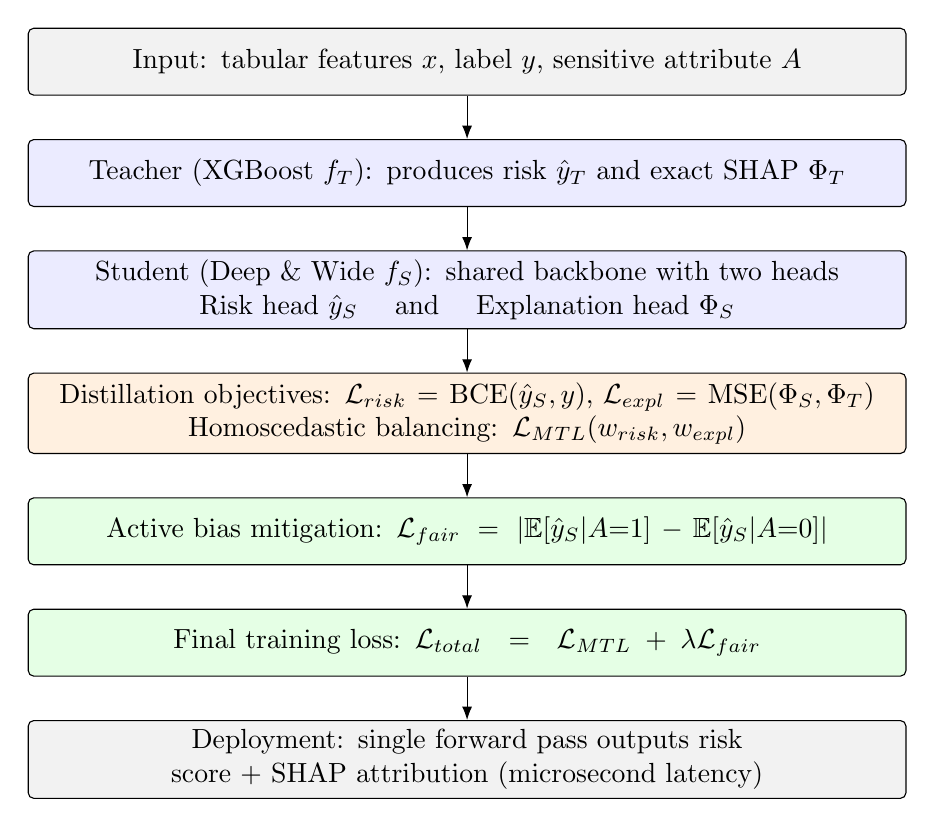
\begin{tikzpicture}[
    >=Latex,
    node distance=0.55cm,
    box/.style={draw, rounded corners=2pt, align=center, minimum height=0.85cm, text width=0.9\columnwidth},
    io/.style={box, fill=gray!10},
    model/.style={box, fill=blue!8},
    loss/.style={box, fill=orange!12},
    fair/.style={box, fill=green!10}
]
\node[io] (input) {Input: tabular features $x$, label $y$, sensitive attribute $A$};
\node[model, below=of input] (teacher) {Teacher (XGBoost $f_T$): produces risk $\hat{y}_T$ and exact SHAP $\Phi_T$};
\node[model, below=of teacher] (student) {Student (Deep \& Wide $f_S$): shared backbone with two heads\\Risk head $\hat{y}_S$ \quad and \quad Explanation head $\Phi_S$};
\node[loss, below=of student] (mtl) {Distillation objectives: $\mathcal{L}_{risk}=\mathrm{BCE}(\hat{y}_S,y)$, $\mathcal{L}_{expl}=\mathrm{MSE}(\Phi_S,\Phi_T)$\\Homoscedastic balancing: $\mathcal{L}_{MTL}(w_{risk},w_{expl})$};
\node[fair, below=of mtl] (fairness) {Active bias mitigation: $\mathcal{L}_{fair}=|\mathbb{E}[\hat{y}_S|A{=}1]-\mathbb{E}[\hat{y}_S|A{=}0]|$};
\node[fair, below=of fairness] (total) {Final training loss: $\mathcal{L}_{total}=\mathcal{L}_{MTL}+\lambda\mathcal{L}_{fair}$};
\node[io, below=of total] (deploy) {Deployment: single forward pass outputs risk score + SHAP attribution (microsecond latency)};

\draw[->] (input) -- (teacher);
\draw[->] (teacher) -- (student);
\draw[->] (student) -- (mtl);
\draw[->] (mtl) -- (fairness);
\draw[->] (fairness) -- (total);
\draw[->] (total) -- (deploy);
\end{tikzpicture}
\caption{Methodology overview of the proposed Teacher--Student distillation pipeline. The Student learns both prediction and explanation tasks from the Teacher under homoscedastic multi-task balancing, while an explicit demographic-parity term enforces fairness during training.}
\label{fig:pipeline}
\end{figure}


To resolve the extreme latency overhead of post-hoc explainers like TreeSHAP in real-time streaming environments, we employ a Knowledge Distillation (KD) framework. In this paradigm, a highly accurate but computationally expensive tree-based ensemble serves as the ``Teacher'' model, while a fast, lightweight Neural Network acts as the ``Student''. 

Let the Teacher model be an XGBoost classifier $f_T$, which processes a tabular feature vector $x \in \mathbb{R}^d$ to output a predicted risk probability $\hat{y}_T$ and a corresponding vector of exact SHAP values $\Phi_T \in \mathbb{R}^d$. The Student model, $f_S$, is a Deep and Wide multi-task neural network parameterized by $\theta$. The architecture consists of a shared representation backbone—comprising fully connected layers with ReLU activations and Dropout for regularization—that bifurcates into two distinct heads:
\begin{itemize}
\item \textbf{Risk Head:} A single-neuron linear layer followed by a Sigmoid activation, optimized to predict the risk probability $\hat{y}_S \in [0,1]$.
\item \textbf{Explanation Head:} A linear layer with $d$ output neurons, optimized to directly output the estimated SHAP values $\Phi_S \in \mathbb{R}^d$.
\end{itemize}

Formally, the shared representation $h^{(L)}$ after $L$ hidden layers is given by:
\begin{equation} %\label{eq:backbone}
    h^{(l)} = \text{ReLU}\left(W^{(l)} h^{(l-1)} + b^{(l)}\right) \quad \text{for } l = 1, \dots, L
\end{equation}
where $h^{(0)} = x$. The network then bifurcates into the dual heads:
\begin{equation*} %\label{eq:riskhead}
    \hat{y}_{S} = \sigma\left(W_{risk} h^{(L)} + b_{risk}\right)\text{ and}
\end{equation*}
\begin{equation*} %\label{eq:explhead}
    \Phi_{S} = W_{expl} h^{(L)} + b_{expl} \text{.}
\end{equation*}

By inferring both the risk score and the feature attributions in a single forward pass, the Student architecture fundamentally bypasses the combinatorial complexity of exact SHAP calculations outlined in (\ref{eq:shap}).

\subsection{Autonomous Loss Balancing}

Training the dual-head Student network requires simultaneously minimizing a classification loss for the risk predictions (Binary Cross-Entropy, or BCE) and a regression loss for the explanatory fidelity (Mean Squared Error, or MSE). Formally, over a mini-batch of size $N$, the base task losses are:

\begin{equation*} %\label{eq:loss_risk}
    \mathcal{L}_{risk} = -\frac{1}{N}\sum_{j=1}^{N} \left[ y^{(j)} \log(\hat{y}_{S}^{(j)}) + (1-y^{(j)}) \log(1-\hat{y}_{S}^{(j)}) \right]\text{ and}
\end{equation*}

\begin{equation*} %\label{eq:loss_expl}
    \mathcal{L}_{expl} = \frac{1}{N}\sum_{j=1}^{N} \left\| \Phi_{S}^{(j)} - \Phi_{T}^{(j)} \right\|_{2}^{2}\text{,}
\end{equation*}

where $y^{(j)}$ represents the ground-truth target label for the $j$-th instance. 

In multi-task learning, assigning static, scalar weights to fundamentally different loss functions (a probability likelihood vs. a continuous magnitude) often results in suboptimal convergence and requires exhaustive grid searches. To circumvent this, we implement Homoscedastic Task Uncertainty \cite{DBLP:journals/corr/KendallGC17}. This approach treats the task-specific uncertainties as learnable parameters, dynamically weighting the losses during backpropagation. 

We define two learnable log-variance parameters, $w_{risk} = \log(\sigma_{risk}^2)$ and $w_{expl} = \log(\sigma_{expl}^2)$, initialized at zero. The autonomous multi-task loss ($\mathcal{L}_{MTL}$) is formulated as:

\begin{equation} \label{eq:mtl}
    \mathcal{L}_{MTL} = \exp(-w_{risk})\mathcal{L}_{risk} + 0.5 w_{risk} + \exp(-w_{expl})\mathcal{L}_{expl} + 0.5 w_{expl}
\end{equation}
This formulation acts as a self-calibrating mechanism. If the MSE explanation loss dominates the gradients, the optimizer autonomously increases $w_{expl}$, penalizing the loss scale while regularizing via the $+ 0.5 w_{expl}$ term. This allows the network to find a natural mathematical equilibrium between predictive accuracy and explanatory fidelity without manual intervention.

\subsection{Active Bias Mitigation via L1 Penalty}
% To resolve the extreme latency overhead of post-hoc explainers like TreeSHAP in real-time streaming environments, we employ a Knowledge Distillation (KD) framework. In this paradigm, a highly accurate but computationally expensive tree-based ensemble serves as the ``Teacher'' model, while a fast, lightweight Neural Network acts as the ``Student''. 

% Let the Teacher model be an XGBoost classifier $f_T$, which processes a tabular feature vector $x \in \mathbb{R}^d$ to output a predicted risk probability $\hat{y}_T$ and a corresponding vector of exact SHAP values $\Phi_T \in \mathbb{R}^d$. The Student model, $f_S$, is a Deep and Wide multi-task neural network parameterized by $\theta$. The architecture consists of a shared representation backbone—comprising fully connected layers with ReLU activations and Dropout for regularization—that bifurcates into two distinct heads:
% \begin{itemize}
%     \item \textbf{Risk Head:} A single-neuron linear layer followed by a Sigmoid activation, optimized to predict the risk probability $\hat{y}_S \in [0,1]$.
%     \item \textbf{Explanation Head:} A linear layer with $d$ output neurons, optimized to directly output the estimated SHAP values $\Phi_S \in \mathbb{R}^d$.
% \end{itemize}
% By inferring both the risk score and the feature attributions in a single forward pass, the Student architecture fundamentally bypasses the combinatorial complexity of exact SHAP calculations.

% \subsection{Autonomous Loss Balancing}

% Training the dual-head Student network requires simultaneously minimizing a classification loss for the risk predictions (Binary Cross-Entropy, or BCE) and a regression loss for the explanatory fidelity (Mean Squared Error, or MSE). Formally, the base task losses are:
% $$
%     \mathcal{L}_{risk} = \text{BCE}(\hat{y}_S, y) \quad \text{and} \quad \mathcal{L}_{expl} = \text{MSE}(\Phi_S, \Phi_T) .
% $$
% where $y$ represents the ground-truth target label. 

% In multi-task learning, assigning static, scalar weights to fundamentally different loss functions (a probability likelihood vs. a continuous magnitude) often results in suboptimal convergence and requires exhaustive grid searches. To circumvent this, we implement Homoscedastic Task Uncertainty \cite{DBLP:journals/corr/KendallGC17}. This approach treats the task-specific uncertainties as learnable parameters, dynamically weighting the losses during backpropagation. 

% We define two learnable log-variance parameters, $w_{risk} = \log(\sigma_{risk}^2)$ and $w_{expl} = \log(\sigma_{expl}^2)$, initialized at zero. The autonomous multi-task loss ($\mathcal{L}_{MTL}$) is formulated as:

% \begin{equation} \label{eq:mtl}
%     \mathcal{L}_{MTL} = \exp(-w_{risk})\mathcal{L}_{risk} + 0.5 w_{risk} + \exp(-w_{expl})\mathcal{L}_{expl} + 0.5 w_{expl}
% \end{equation}
% This formulation acts as a self-calibrating mechanism. If the MSE explanation loss dominates the gradients, the optimizer autonomously increases $w_{expl}$, penalizing the loss scale while regularizing via the $+ 0.5 w_{expl}$ term. This allows the network to find a natural mathematical equilibrium between predictive accuracy and explanatory fidelity without manual intervention.

% \subsection{Active Bias Mitigation via L1 Penalty}

Historical financial datasets inherently contain structural biases against protected minority groups. To actively mitigate disparate impact during distillation, we introduce a Demographic Parity (DP) constraint. Let $A \in \{0, 1\}$ denote a binary sensitive attribute (e.g., age, nationality), where $A=1$ indicates the protected minority class.

% Initial attempts to enforce fairness utilized a squared (L2) penalty:
% \begin{equation}
%     \mathcal{L}_{DP-L2} = \left( \mathbb{E}[\hat{y}_S | A=1] - \mathbb{E}[\hat{y}_S | A=0] \right)^2
% \end{equation}
Initial attempts to enforce fairness utilized a squared (L2) penalty. However, evaluating this constraint on highly imbalanced mini-batches proved mathematically volatile. In batches with severe minority underrepresentation, the sample mean $\mathbb{E}[\hat{y}_S | A=1]$ becomes highly susceptible to statistical noise. The L2 formulation exponentially amplified this noise, resulting in violent gradient explosions and model divergence.

To stabilize the optimization trajectory, we substitute the sledgehammer of an L2 penalty for the precision of an L1-norm (Absolute Difference) penalty. Furthermore, we implement a ``Safety Net'' heuristic: the fairness penalty is entirely masked (set to zero) for any mini-batch containing fewer than five instances of either demographic group, ensuring gradients are only calculated from statistically viable samples. The stabilized fairness loss is defined as:
\begin{equation} \label{eq:fair}
    \mathcal{L}_{fair} = \begin{cases} 
      \left| \mathbb{E}[\hat{y}_S | A=1] - \mathbb{E}[\hat{y}_S | A=0] \right| & \text{if } \sum \mathbb{I}(A=1) \ge 5 \text{ and } \sum \mathbb{I}(A=0) \ge 5 \\
      0 & \text{otherwise}
   \end{cases}
\end{equation}

Unlike the predictive likelihoods in (\ref{eq:mtl}), the fairness constraint (\ref{eq:fair}) is not a probability distribution and thus cannot be natively balanced via homoscedastic uncertainty. Instead, it must act as a strict regulatory constraint. 

We apply an explicit Lagrangian multiplier ($\lambda = 2.5$) to form the final hybrid loss objective:

$
    \mathcal{L}_{total} = \mathcal{L}_{MTL} + \lambda \mathcal{L}_{fair}.
$

This hybrid architecture ensures the optimizer gently but constantly pushes the latent representations toward equity, significantly suppressing the demographic gap without destabilizing the predictive learning dynamics.



\section{EXPERIMENTAL SETUP}
\label{sec:experimental_setup}
To ensure reproducibility and contextualize the empirical results, we detail the datasets, preprocessing, fairness definitions, and training dynamics used in all notebook experiments.

\subsection{Datasets and Preprocessing}
We validate the proposed pipeline on three benchmark financial datasets using stratified 80/20 train/test splits with fixed seed ($42$) for all runs.  
\begin{itemize}
    \item \textbf{Bank Marketing (UCI 222):} 45,211 records (train shape: 36,168). Categorical features are one-hot encoded and all inputs are standardized; final input dimensionality is 38.
    \item \textbf{German Credit (UCI 144):} 1,000 records (train shape: 800). Categorical fields are label-encoded and inputs are standardized; final input dimensionality is 20.
    \item \textbf{UCI Credit Card Default (UCI 350):} 30,000 records (train shape: 24,000). Inputs are standardized; final input dimensionality is 23.
\end{itemize}

\subsection{Defining the Protected Attributes}
To evaluate and actively mitigate disparate impact, each dataset uses a binary sensitive attribute ($A$):
\begin{itemize}
    \item \textbf{Bank Marketing:} Seniors ($A=1$ if age $>60$).
    \item \textbf{German Credit:} Foreign-worker subgroup ($A=1$ if \texttt{foreign\_worker} equals the minority encoded group used in the notebooks).
    \item \textbf{UCI Credit Card Default:} Education subgroup ($A=1$ if \texttt{EDUCATION} $=2$, i.e., University level), matching the notebook fairness target.
\end{itemize}

\subsection{Model Configuration and Training Dynamics}
\subsubsection{The Teacher} 
The baseline predictions and ground-truth explanations were generated using an XGBoost classifier configured with 100 estimators, a maximum depth of 4, and a learning rate of 0.1. Exact explanations for the training and testing sets were extracted offline via TreeSHAP \cite{NIPS2017_8a20a862}. We emphasize that only the Student's \emph{explanation} head is distilled from the Teacher; the \emph{risk} head is trained directly on the ground-truth labels via BCE. Consequently the framework is a label-supervised multi-task model rather than a pure soft-label distillation of the Teacher's predictions, a distinction that matters when interpreting the accuracy comparisons in Section~\ref{sec:results}. To verify that the fixed Teacher is a fair reference, we additionally performed a randomized 3-fold cross-validated hyperparameter search; tuning changed the Teacher's test AUC only marginally (German Credit $0.8088\!\to\!0.8117$, UCI Credit Card $0.7778\!\to\!0.7800$, Bank Marketing $0.9286\!\to\!0.9343$) and the tuned Teacher outperforms the Student on every dataset.

\subsubsection{The Student} 
The distilled network utilizes a Deep and Wide Multi-Layer Perceptron (MLP) architecture. The shared backbone consists of hidden layers [256, 128, 64] utilizing ReLU activations and Dropout ($p=0.2$). This capacity ensures high approximation fidelity for complex TreeSHAP patterns, while the dropout effectively regularizes the network against noise in the continuous targets.

\subsubsection{Training Dynamics and Batch Stabilization} 
The Student was trained using the Adam optimizer (learning rate $1e-3$). A critical empirical finding during optimization was the severe sensitivity of the L1 Demographic Parity penalty to mini-batch sizes. Because protected groups constitute a tiny fraction of the data (e.g., Seniors represent only $\sim$2-3\% of the Bank Marketing dataset), standard batch sizes (e.g., $n=64$) frequently resulted in batches with zero or near-zero minority representation, causing gradient explosion and model divergence. 

To ensure statistical viability for the fairness constraint, we scaled the batch size significantly. The headline configuration uses $n=512$, 1200 epochs, and seed 42, with two matched runs per dataset: \textit{baseline} ($\lambda=0$) and \textit{fairness-constrained} ($\lambda=2.5$). This large-batch protocol was instrumental in stabilizing fairness gradients and allowing the homoscedastic uncertainty parameters to converge smoothly.

Beyond these single headline runs, Section~\ref{sec:simulation} reports a replicated, scenario-based simulation experiment. There, each scenario is executed under multiple independent seeds and responses are summarized as means with 95\% confidence intervals, so that systematic factor effects are separated from run-to-run stochastic variation. German Credit is run at the full budget with five seeds and the complete factor grid; for the larger UCI Credit Card and Bank Marketing datasets a focused factor grid (fairness pressure, batch size, protected-group prevalence) is run with three seeds at a reduced epoch budget (60--70 epochs). For these two datasets the simulation results characterize \emph{trends} (whose direction is robust to the epoch budget) rather than full-budget point estimates; the headline Table~\ref{tab:main_results} values remain the 1200-epoch runs.

\subsection{Hardware Environment}
All experiments were conducted on a local machine to strictly simulate a constrained production environment, mirroring the resource limitations often found in edge-inference or containerized banking microservices.
\begin{itemize}
    \item \textbf{Device:} MacBook Pro (Late 2024).
    \item \textbf{Processor:} Apple M4 Chip (10-core CPU: 4 performance and 6 efficiency cores) based on ARM64 architecture. 
    \item \textbf{Memory:} 24 GB Unified Memory.
    \item \textbf{Software Stack:} PyTorch 2.4. While the framework is optimized for the MPS (Metal Performance Shaders) backend, all latency benchmarking was restricted strictly to sequential CPU execution to ensure a fair, worst-case comparison against standard post-hoc baselines.
\end{itemize}
The replicated simulation experiment, batched-throughput benchmark, and discrete-event deployment simulation reported in Sections~\ref{sec:simulation}--\ref{sec:deployment} were executed in a separate constrained CPU environment (4-core ARM64, PyTorch 2.2, single-threaded BLAS); the device is stated explicitly with each result.

\section{RESULTS}
\label{sec:results}
Table~\ref{tab:main_results} reports the apples-to-apples comparison from the three notebooks, where architecture, split, and optimization settings are fixed and only $\lambda_{fair}$ changes from 0.0 to 2.5.

\begin{table}[htb]
\centering
\caption{Main predictive/fidelity/fairness results at the headline configuration (single run per cell, $n=512$, 1200 epochs, seed 42; baseline $\lambda{=}0$ vs fairness-constrained $\lambda{=}2.5$). Lower DP gap is better. Multi-seed means with 95\% confidence intervals are reported in Section~\ref{sec:simulation}; the small AUC differences here are within that replication noise.}
\label{tab:main_results}
\begin{tabular}{lccc}
\hline
Dataset & AUC & SHAP $R^2$ & DP gap \\ \hline
Bank Marketing (baseline) & 0.8959 & 0.5711 & 0.3762 \\
Bank Marketing (fairness) & 0.9066 & 0.5782 & 0.0740 \\
German Credit (baseline) & 0.8170 & 0.5421 & 0.1117 \\
German Credit (fairness) & 0.7970 & 0.5219 & 0.0756 \\
UCI Credit Card (baseline) & 0.7276 & 0.7958 & 0.0309 \\
UCI Credit Card (fairness) & 0.7486 & 0.8395 & 0.0103 \\ \hline
\end{tabular}
\end{table}

Table~\ref{tab:main_results} reports single runs at the headline configuration; we caution against over-interpreting the small AUC differences, which the replicated experiment in Section~\ref{sec:simulation} shows to be within run-to-run noise. With that caveat, two robust observations emerge. First, active mitigation reduces demographic disparity in all three datasets (largest drop in Bank Marketing: $0.3762 \rightarrow 0.0740$). Second, the effect on utility is genuinely dataset-dependent and is governed by how well the protected group is represented: for the balanced UCI Credit Card group the fairness term is essentially accuracy-neutral, whereas for the small Bank Marketing (seniors, $\sim$2.7\%) and German Credit groups it interacts strongly with optimization stability.

We explicitly correct one impression from the submitted single-run numbers: the apparent rise in AUC under fairness (e.g., Bank Marketing $0.8959\rightarrow0.9066$) is \emph{not} a fairness-driven accuracy gain. Because the risk head is label-supervised (Section~\ref{sec:experimental_setup}), the comparison is between two runs of the same network differing only in $\lambda$; under five-seed replication the AUC differences are not statistically significant (Section~\ref{sec:simulation}), and on Bank Marketing the multi-seed trend in fact shows AUC \emph{decreasing} with fairness pressure. Moreover, the (tuned) Teacher outperforms the Student on every dataset, so the Student is not a state-of-the-art accuracy model whose ranking would meaningfully ``improve'' through regularization. We therefore reframe the contribution as bias mitigation \emph{at no significant accuracy cost} in the favorable regime, with an explicit ``cost of fairness'' where the protected group is scarce.

\begin{figure}[htb]
\centering
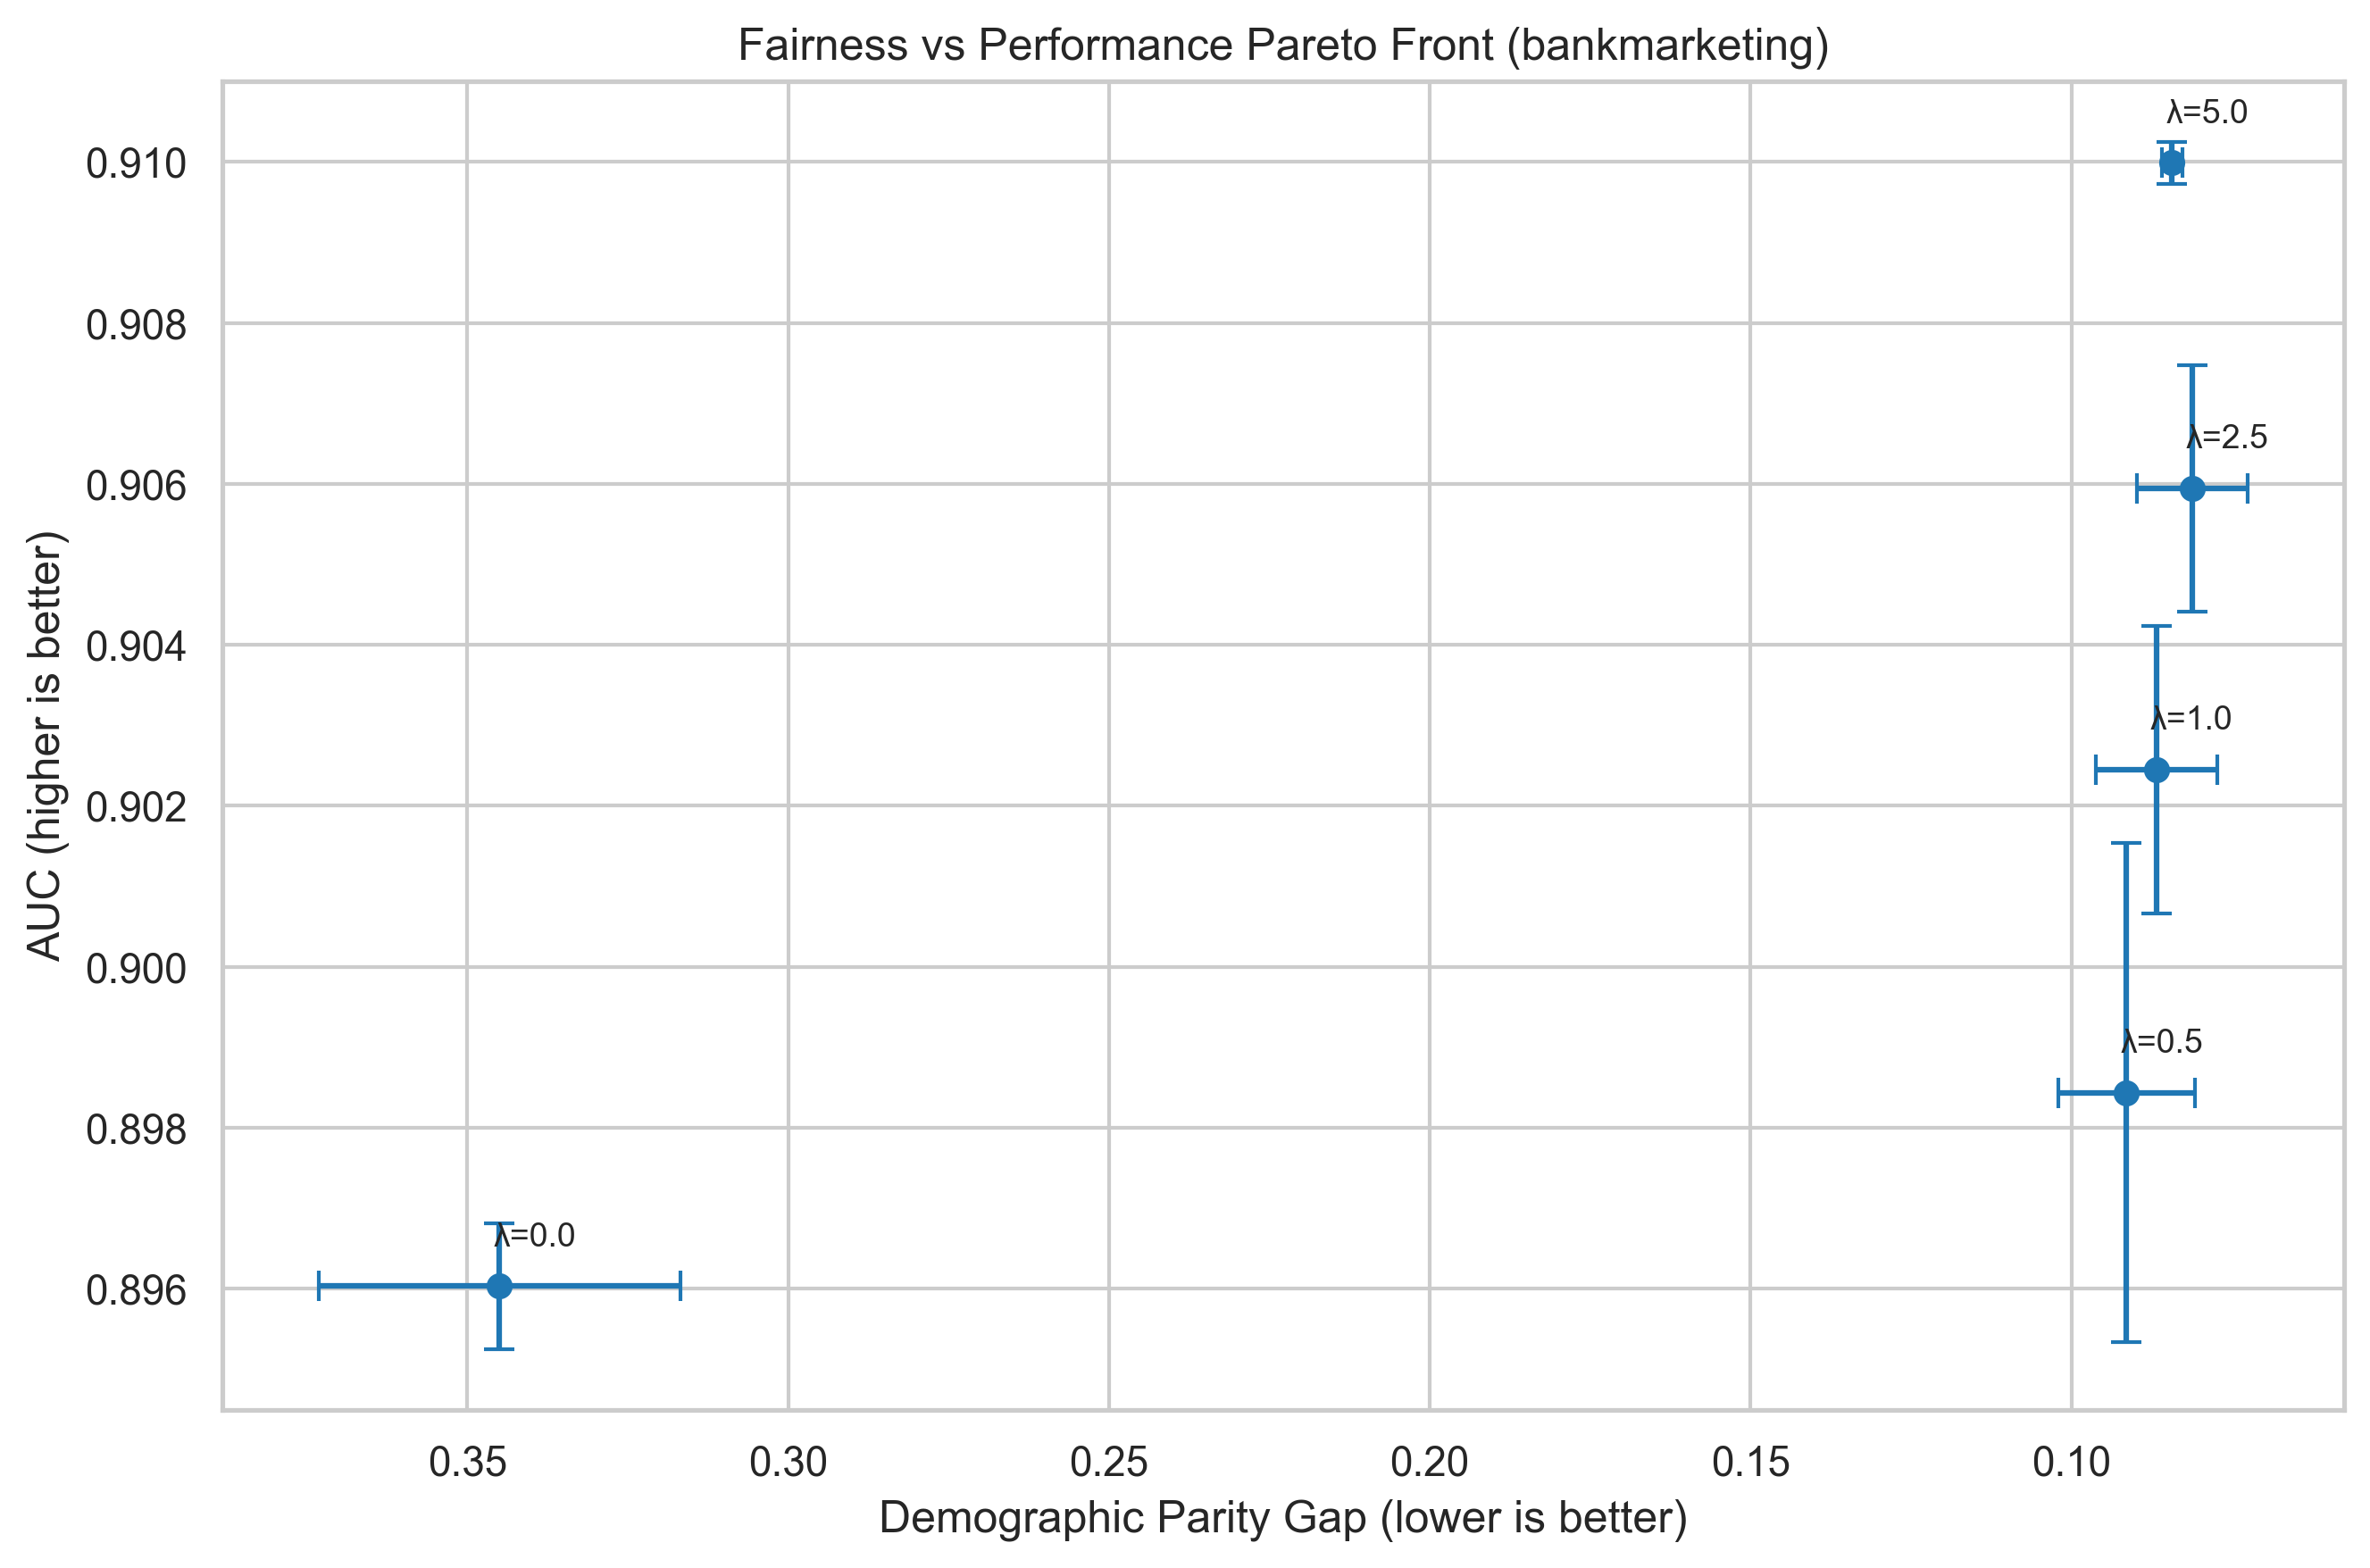
\includegraphics[width=0.32\columnwidth]{fig_wsc_eloi/fig_results_pareto_bankmarketing.png}\hfill
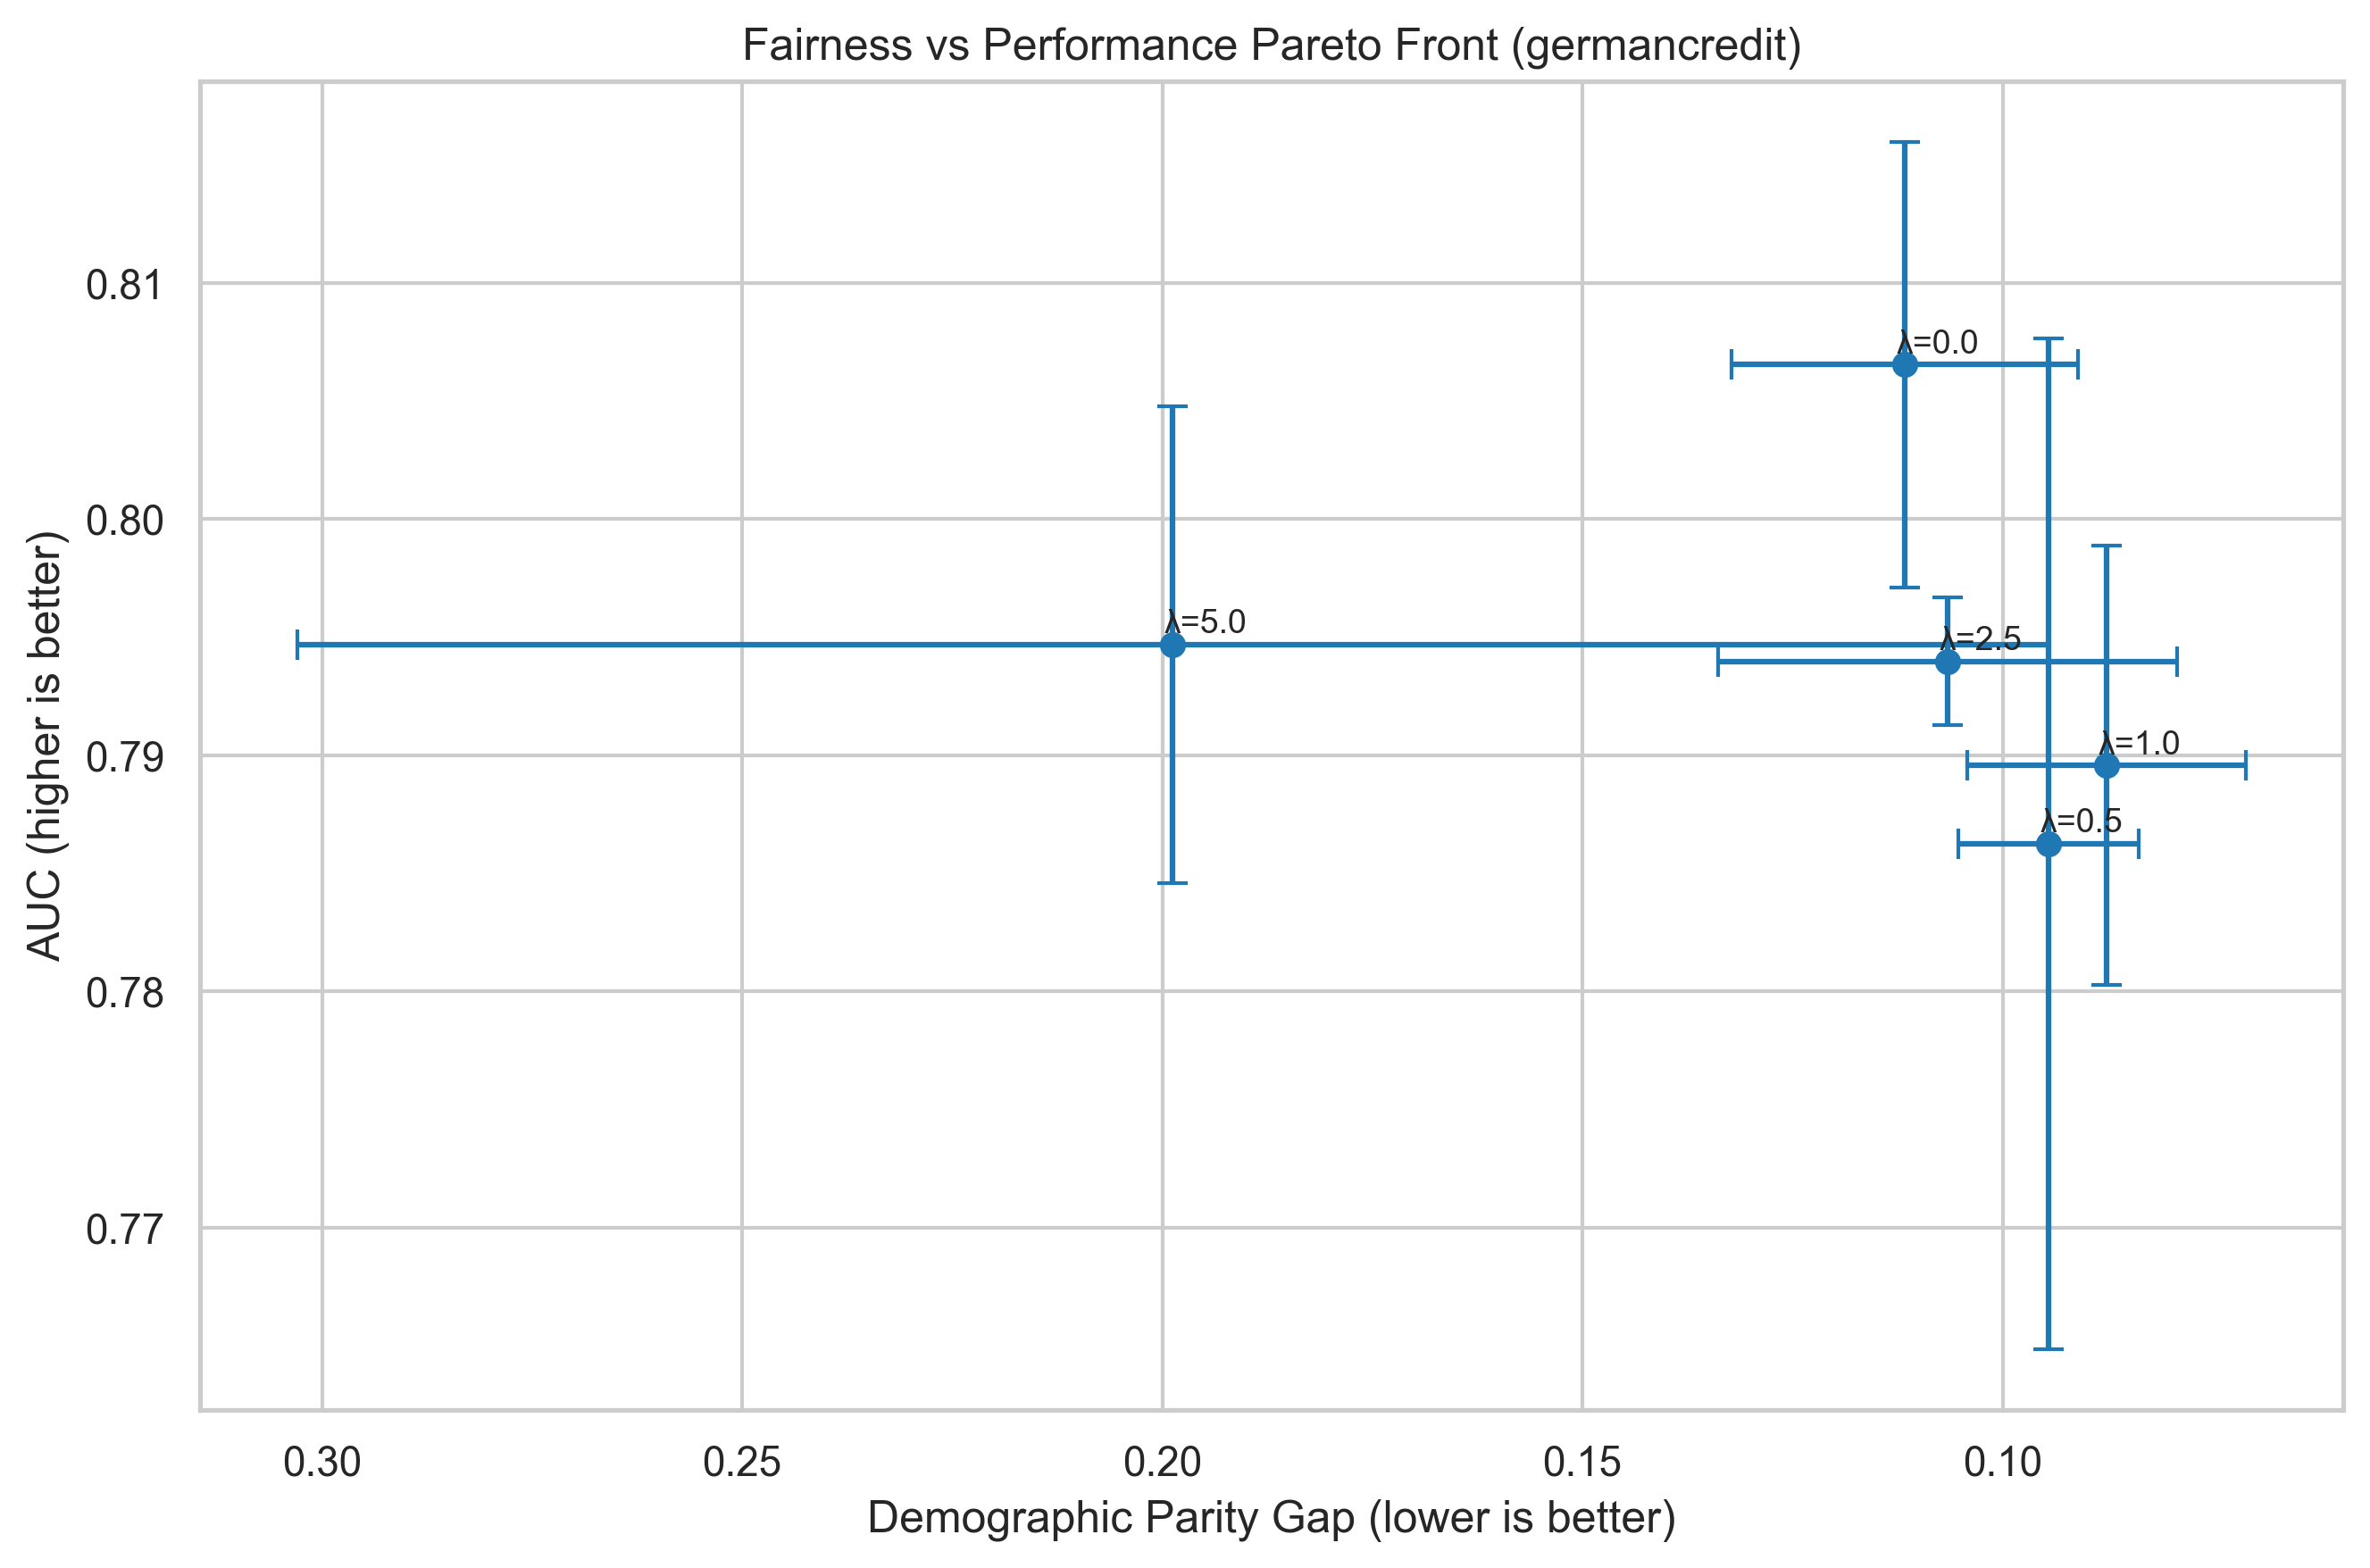
\includegraphics[width=0.32\columnwidth]{fig_wsc_eloi/fig_results_pareto_germancredit.png}\hfill
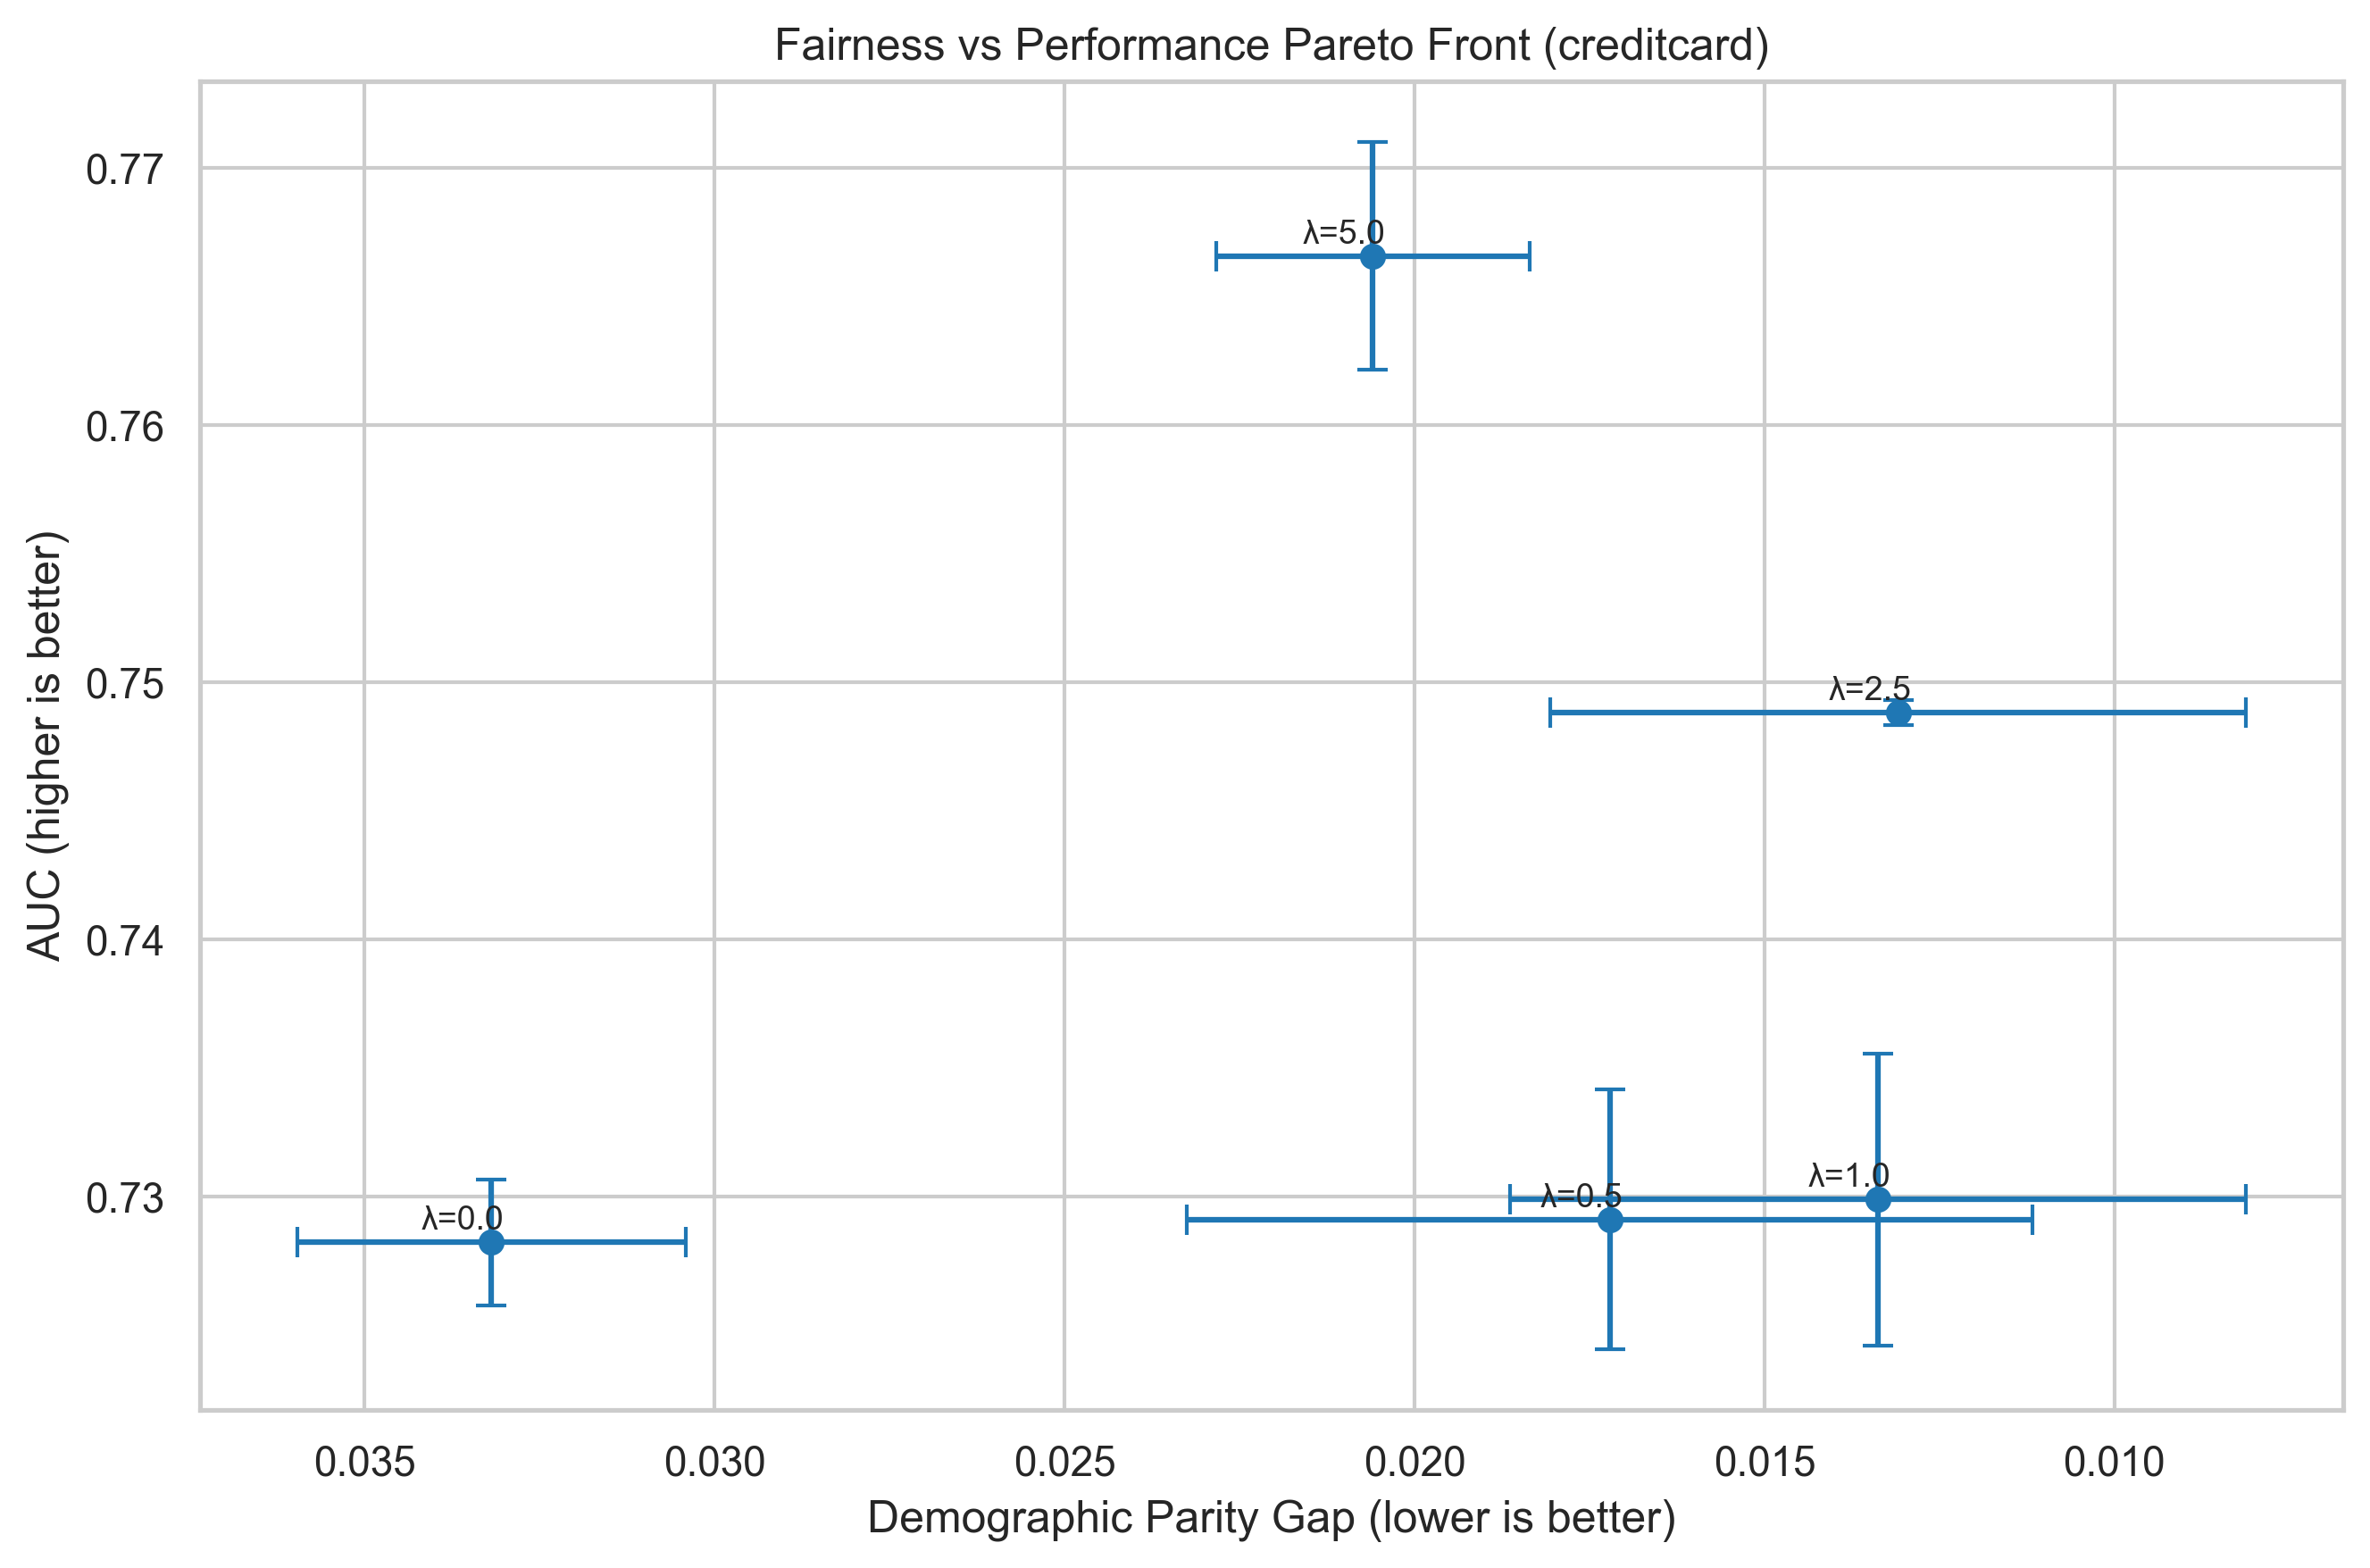
\includegraphics[width=0.32\columnwidth]{fig_wsc_eloi/fig_results_pareto_creditcard.png}
\caption{Fairness--performance Pareto fronts (DP gap vs AUC) across datasets: Bank Marketing (left), German Credit (center), and UCI Credit Card (right).}
\label{fig:pareto_results}
\end{figure}

Latency measurements from the notebooks are reported in Table~\ref{tab:latency_results}, and the latency distribution is visualized in Figure~\ref{fig:latency_distribution}. In all cases, the Student produces risk score and explanation in a single forward pass with sub-millisecond tail latency. The ``Speedup vs SHAP ref.'' column is computed against a conservative $0.5$ ms post-hoc reference drawn from the literature; we caution that it should be read as a reference-relative figure, not as the speedup over our particular Teacher. Indeed, for the \emph{submitted} small Teacher (100 trees, depth 4) a single-instance TreeSHAP call costs only $\approx0.17$ ms, so the per-request advantage over that Teacher is modest ($\approx1.2\times$); the order-of-magnitude advantage materializes for accurate, larger ensembles and, more importantly, under concurrent load (Section~\ref{sec:deployment}).

\begin{table}[htb]
\centering
\caption{Inference latency of the distilled Student (CPU Benchmark).}
\label{tab:latency_results}
\begin{tabular}{lcc}
\hline
Dataset & Student P99 (ms) & Speedup vs SHAP ref. \\ \hline
Bank Marketing & 0.136 & 3,676$\times$ \\
German Credit & 0.032 & 15,625$\times$ \\
UCI Credit Card & 0.053 & 9,434$\times$ \\ \hline
\end{tabular}
\end{table}


\begin{figure}[htb]
\centering
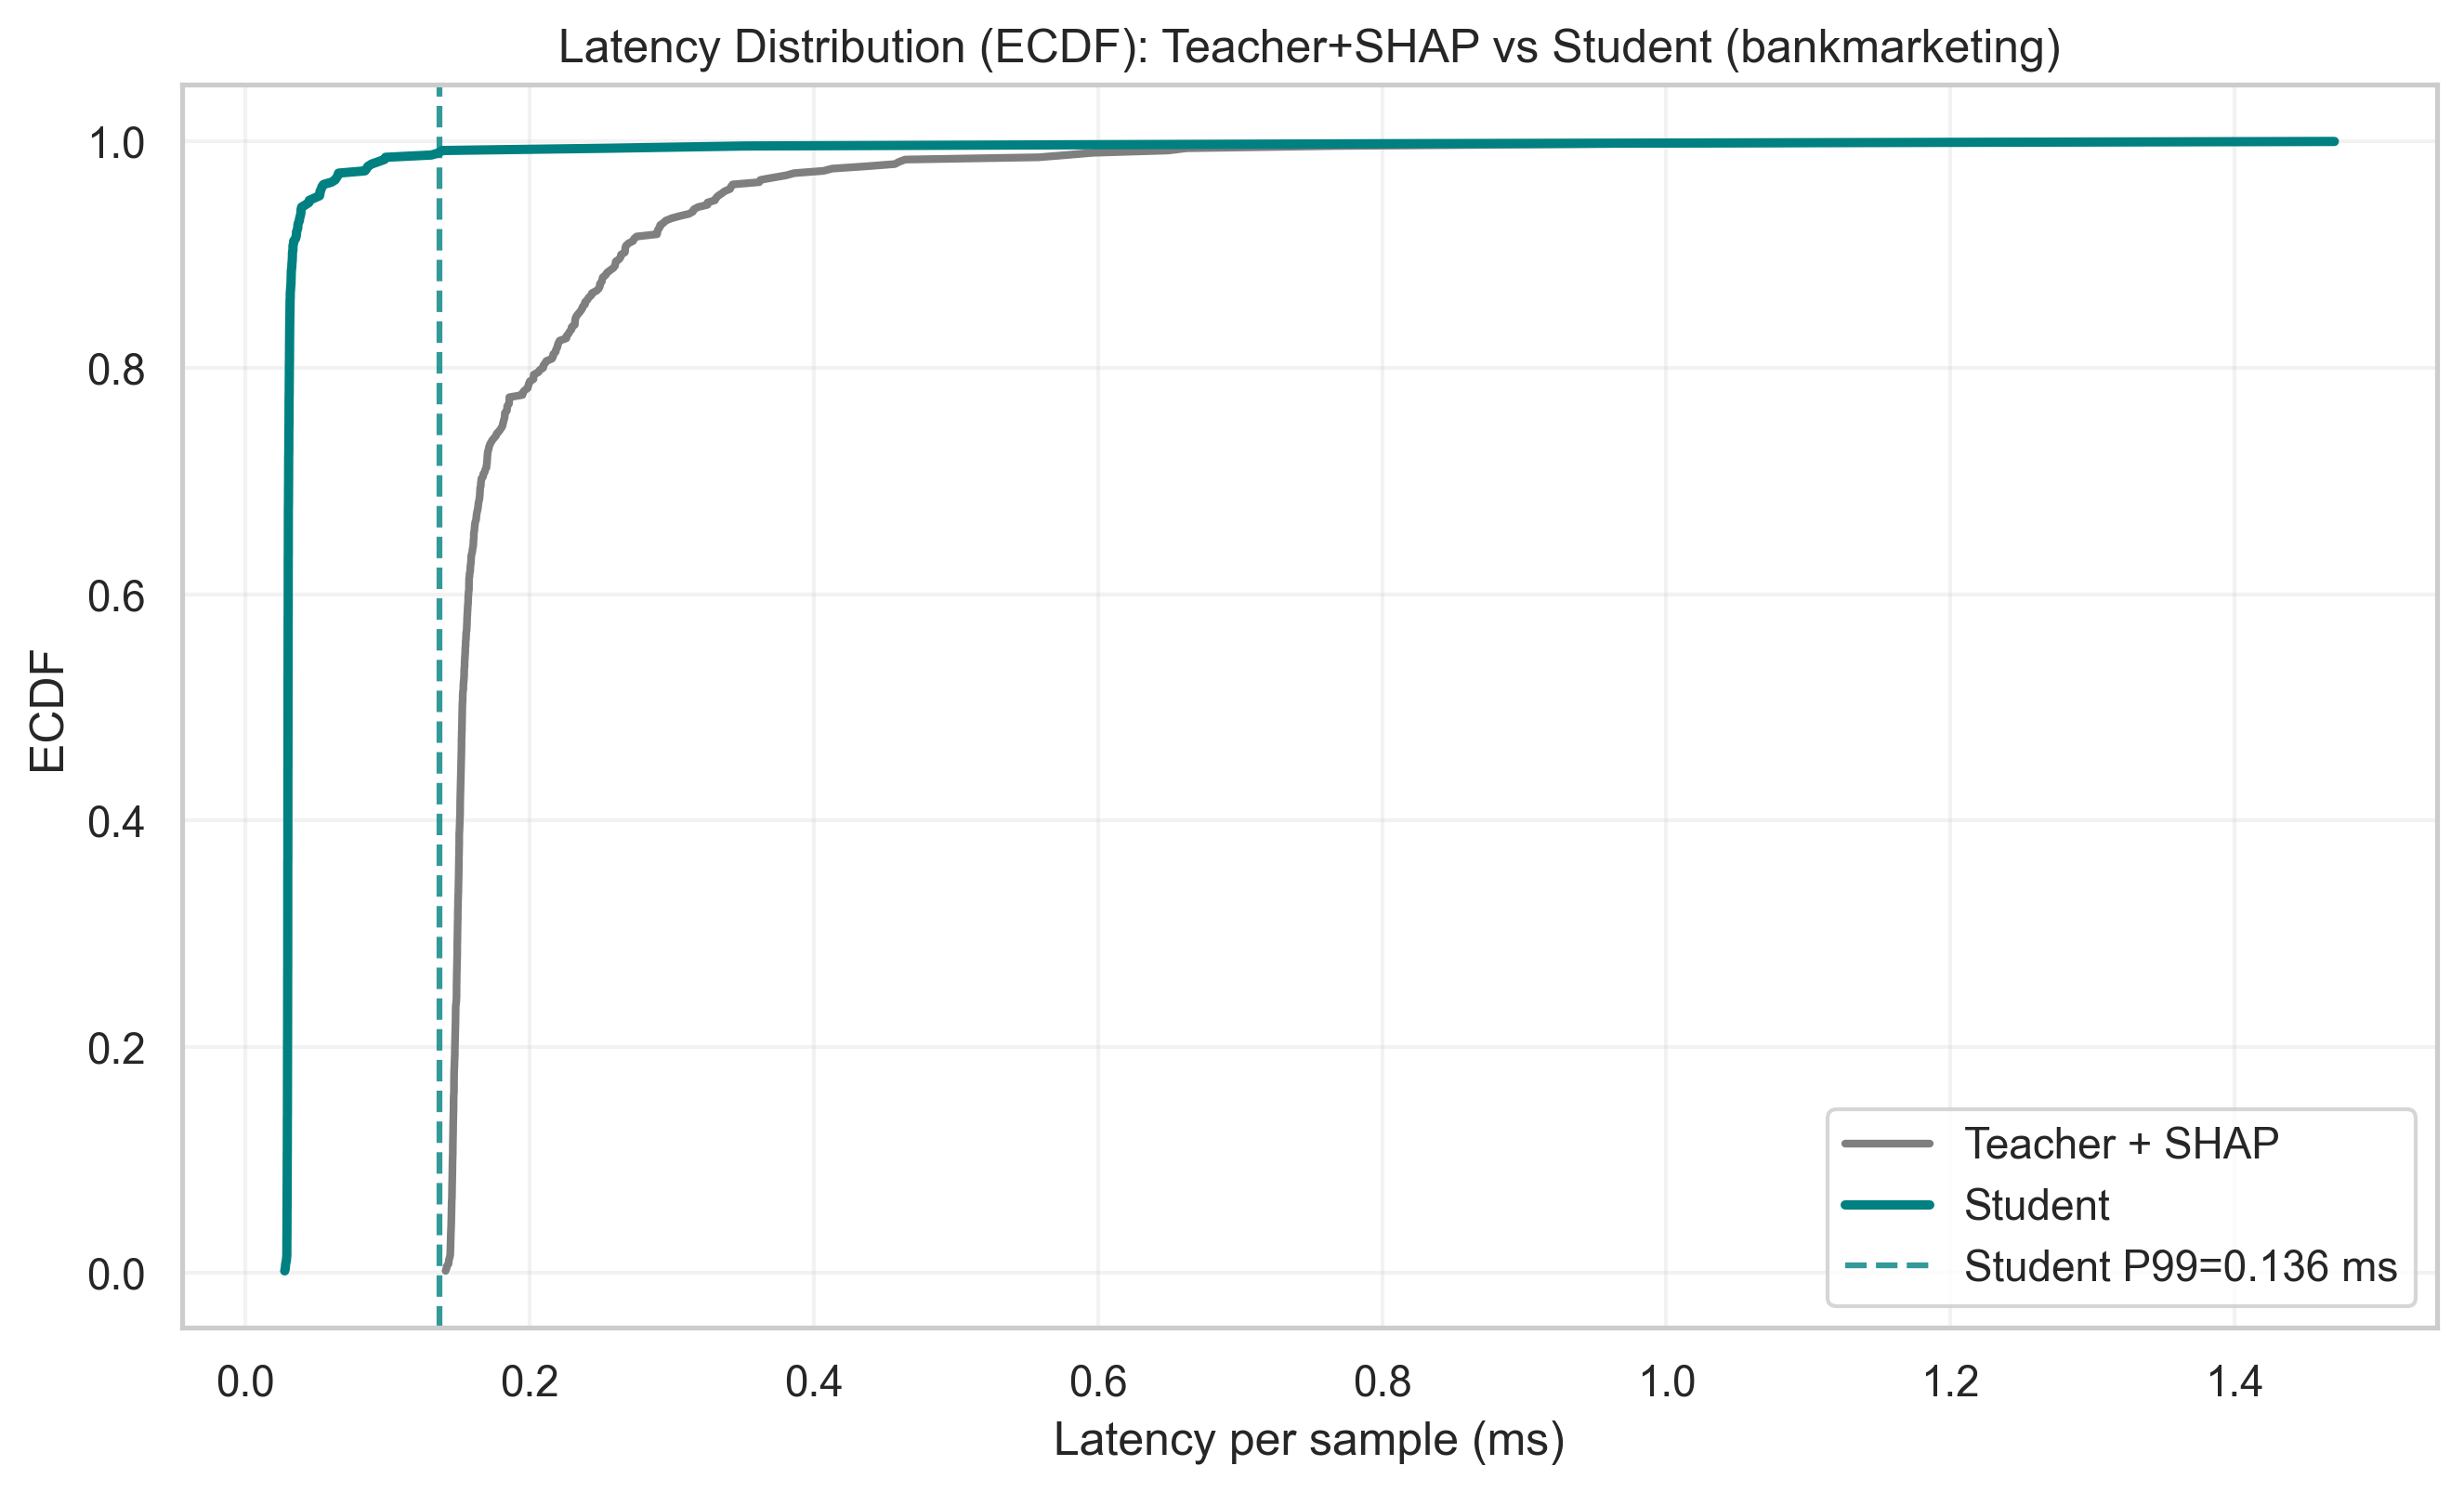
\includegraphics[width=0.32\columnwidth]{fig_wsc_eloi/fig_results_latency_ecdf_bankmarketing.png}\hfill
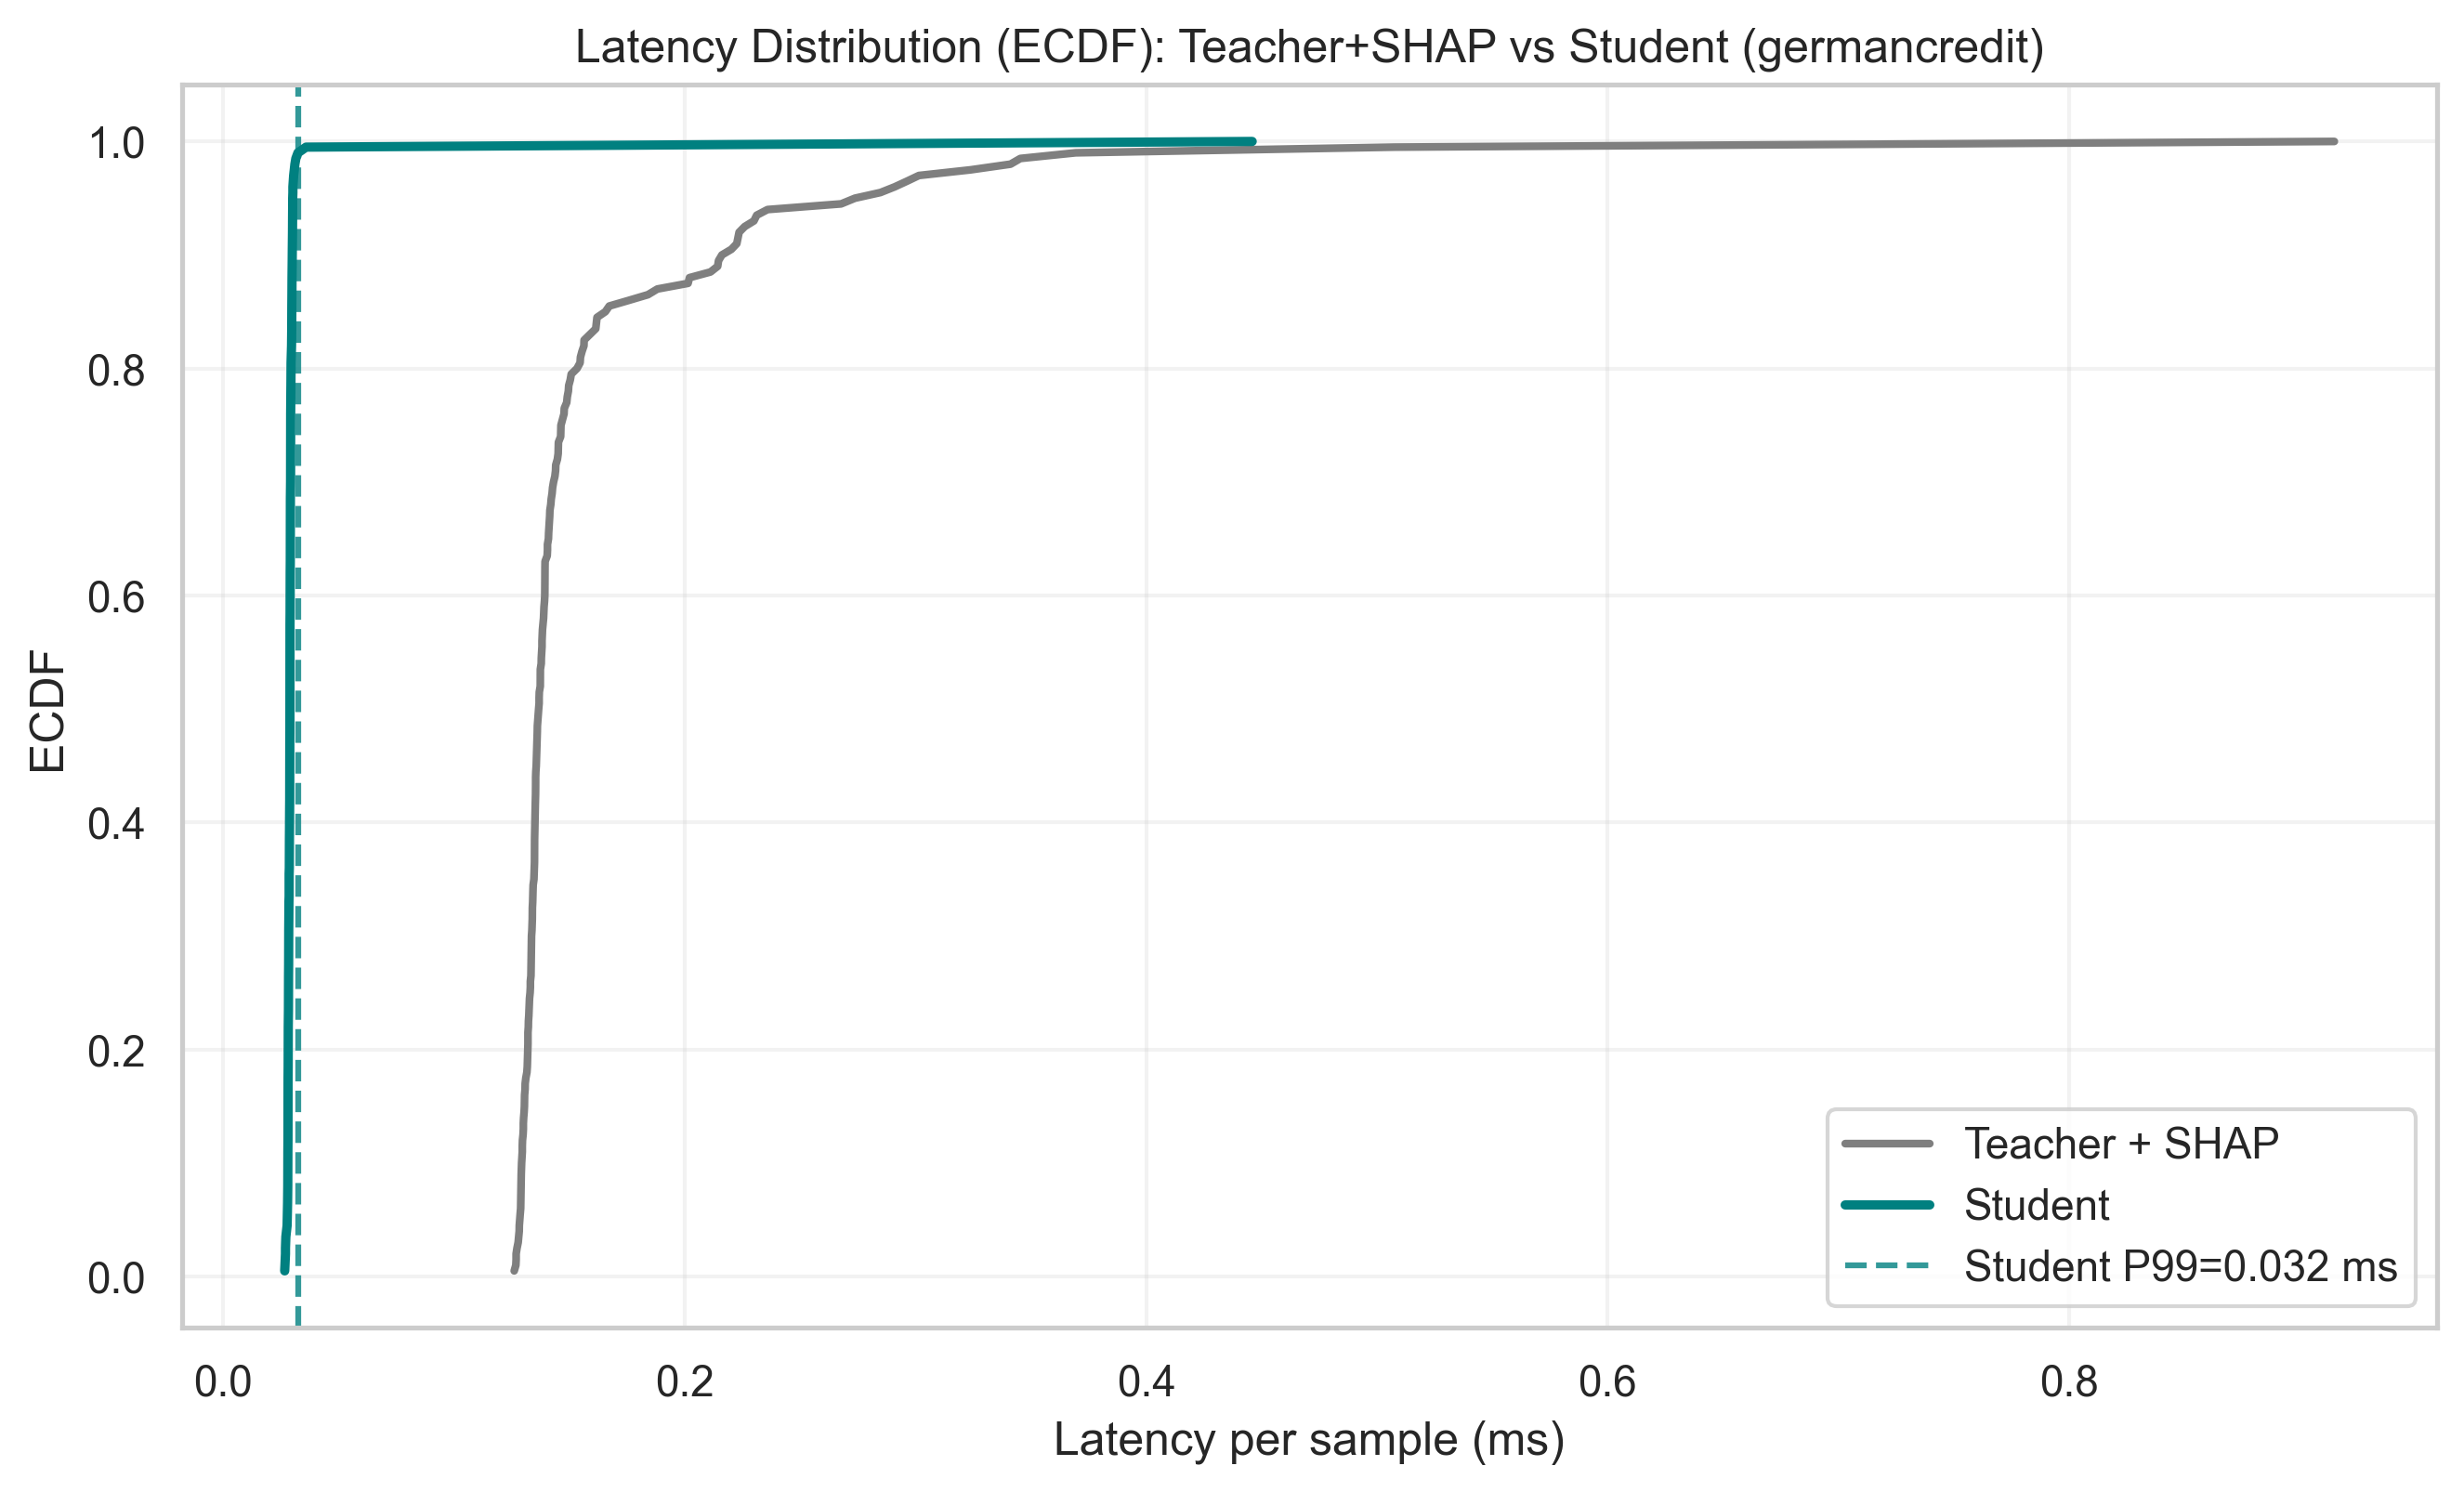
\includegraphics[width=0.32\columnwidth]{fig_wsc_eloi/fig_results_latency_ecdf_germancredit.png}\hfill
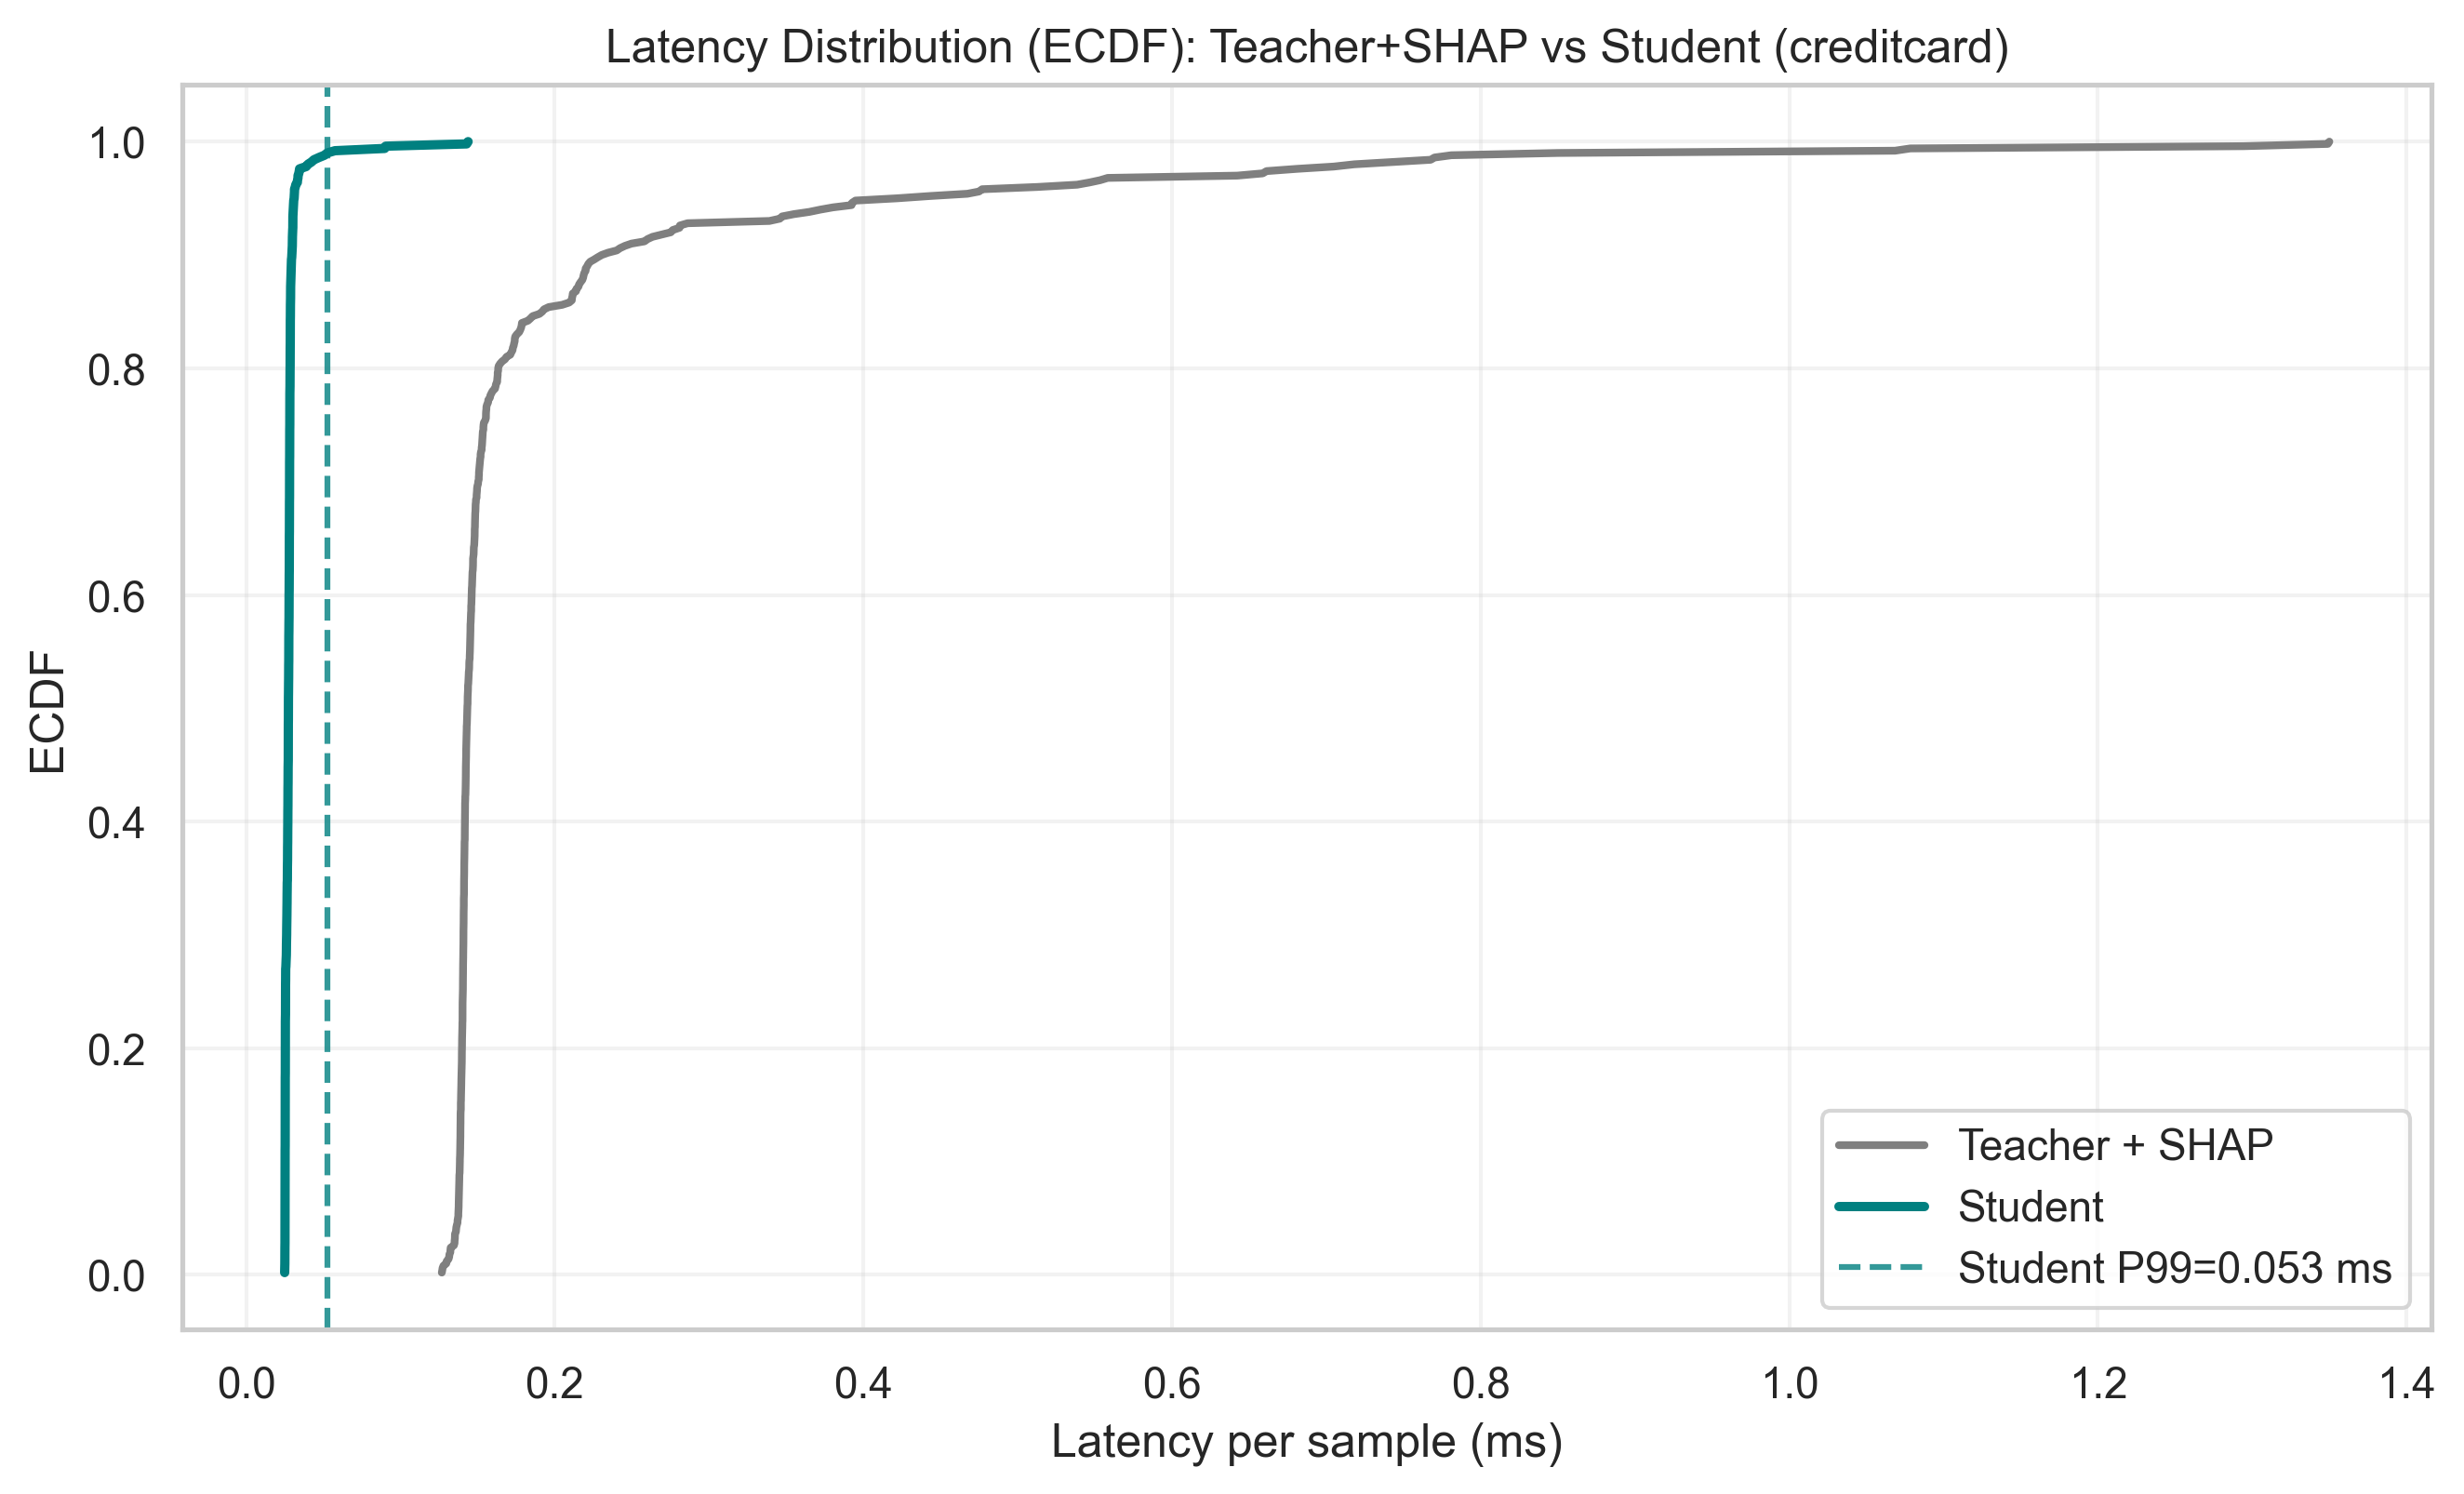
\includegraphics[width=0.32\columnwidth]{fig_wsc_eloi/fig_results_latency_ecdf_creditcard.png}
\caption{Latency ECDF comparison (Teacher+SHAP vs Student) across datasets: Bank Marketing (left), German Credit (center), and UCI Credit Card (right). In all cases, the Student achieves a substantially better latency profile.}
\label{fig:latency_distribution}
\end{figure}

\begin{figure}[htb]
\centering
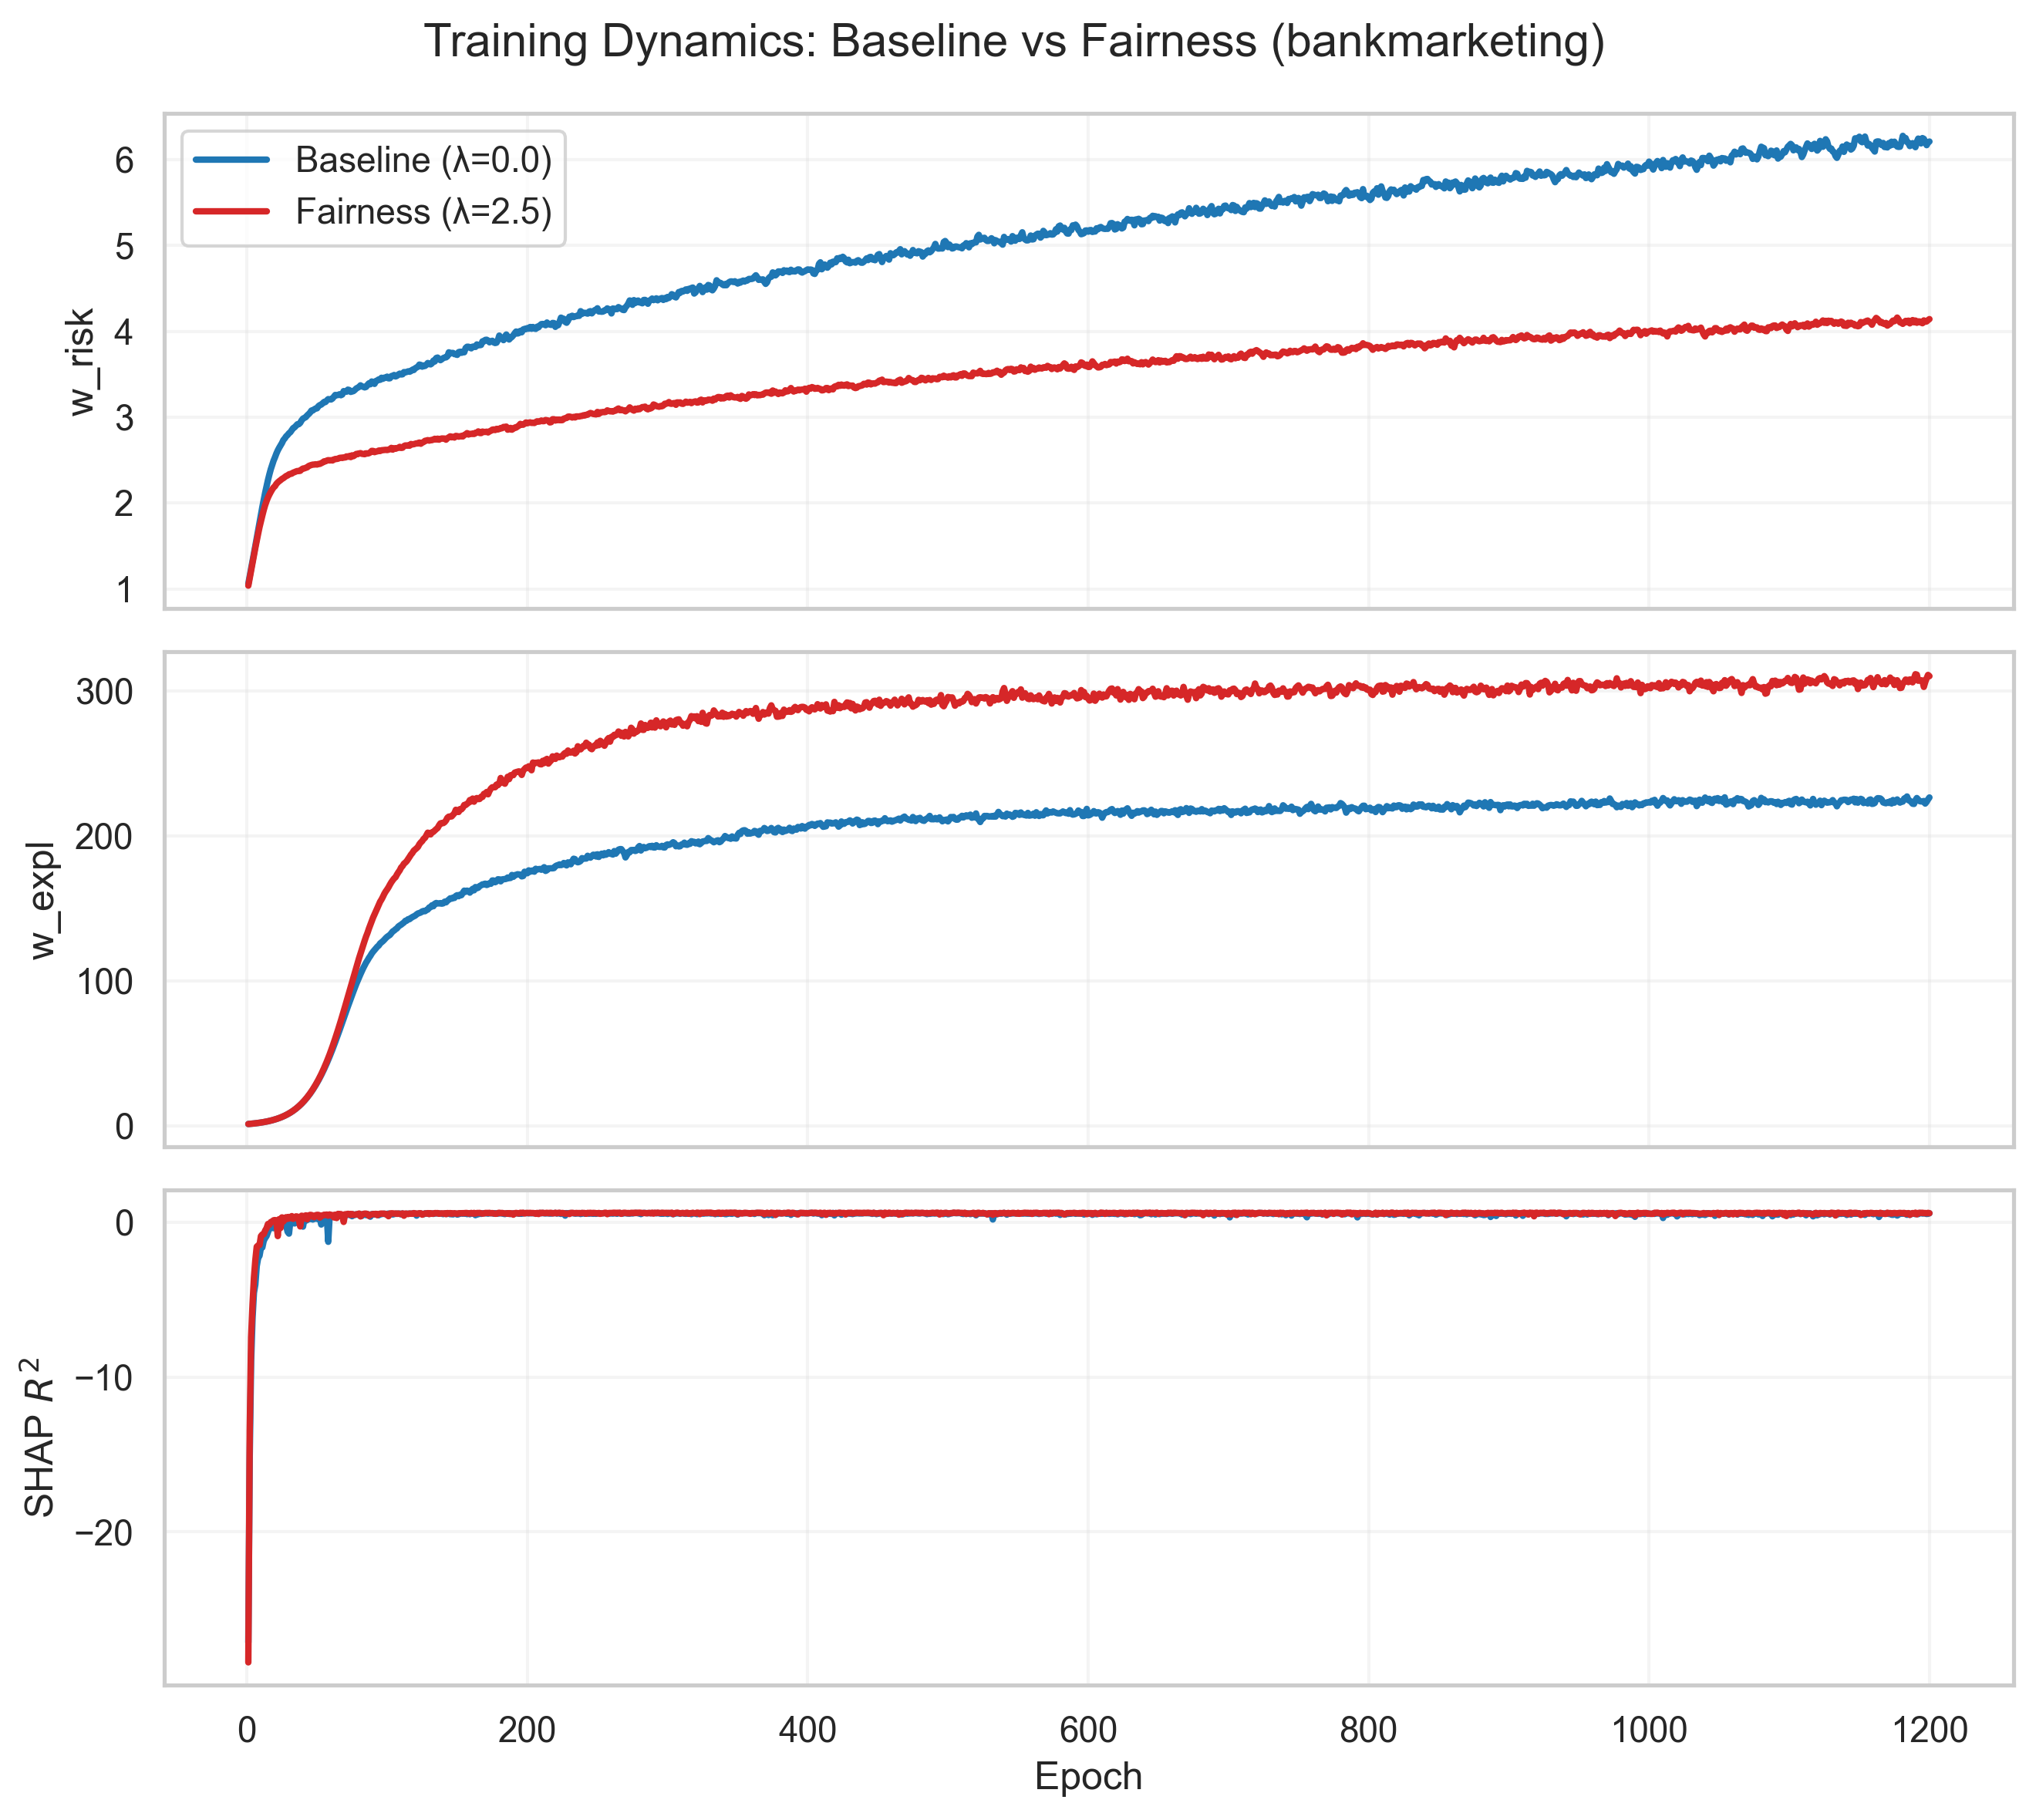
\includegraphics[width=0.32\columnwidth]{fig_wsc_eloi/fig_results_training_dynamics_bankmarketing.png}\hfill
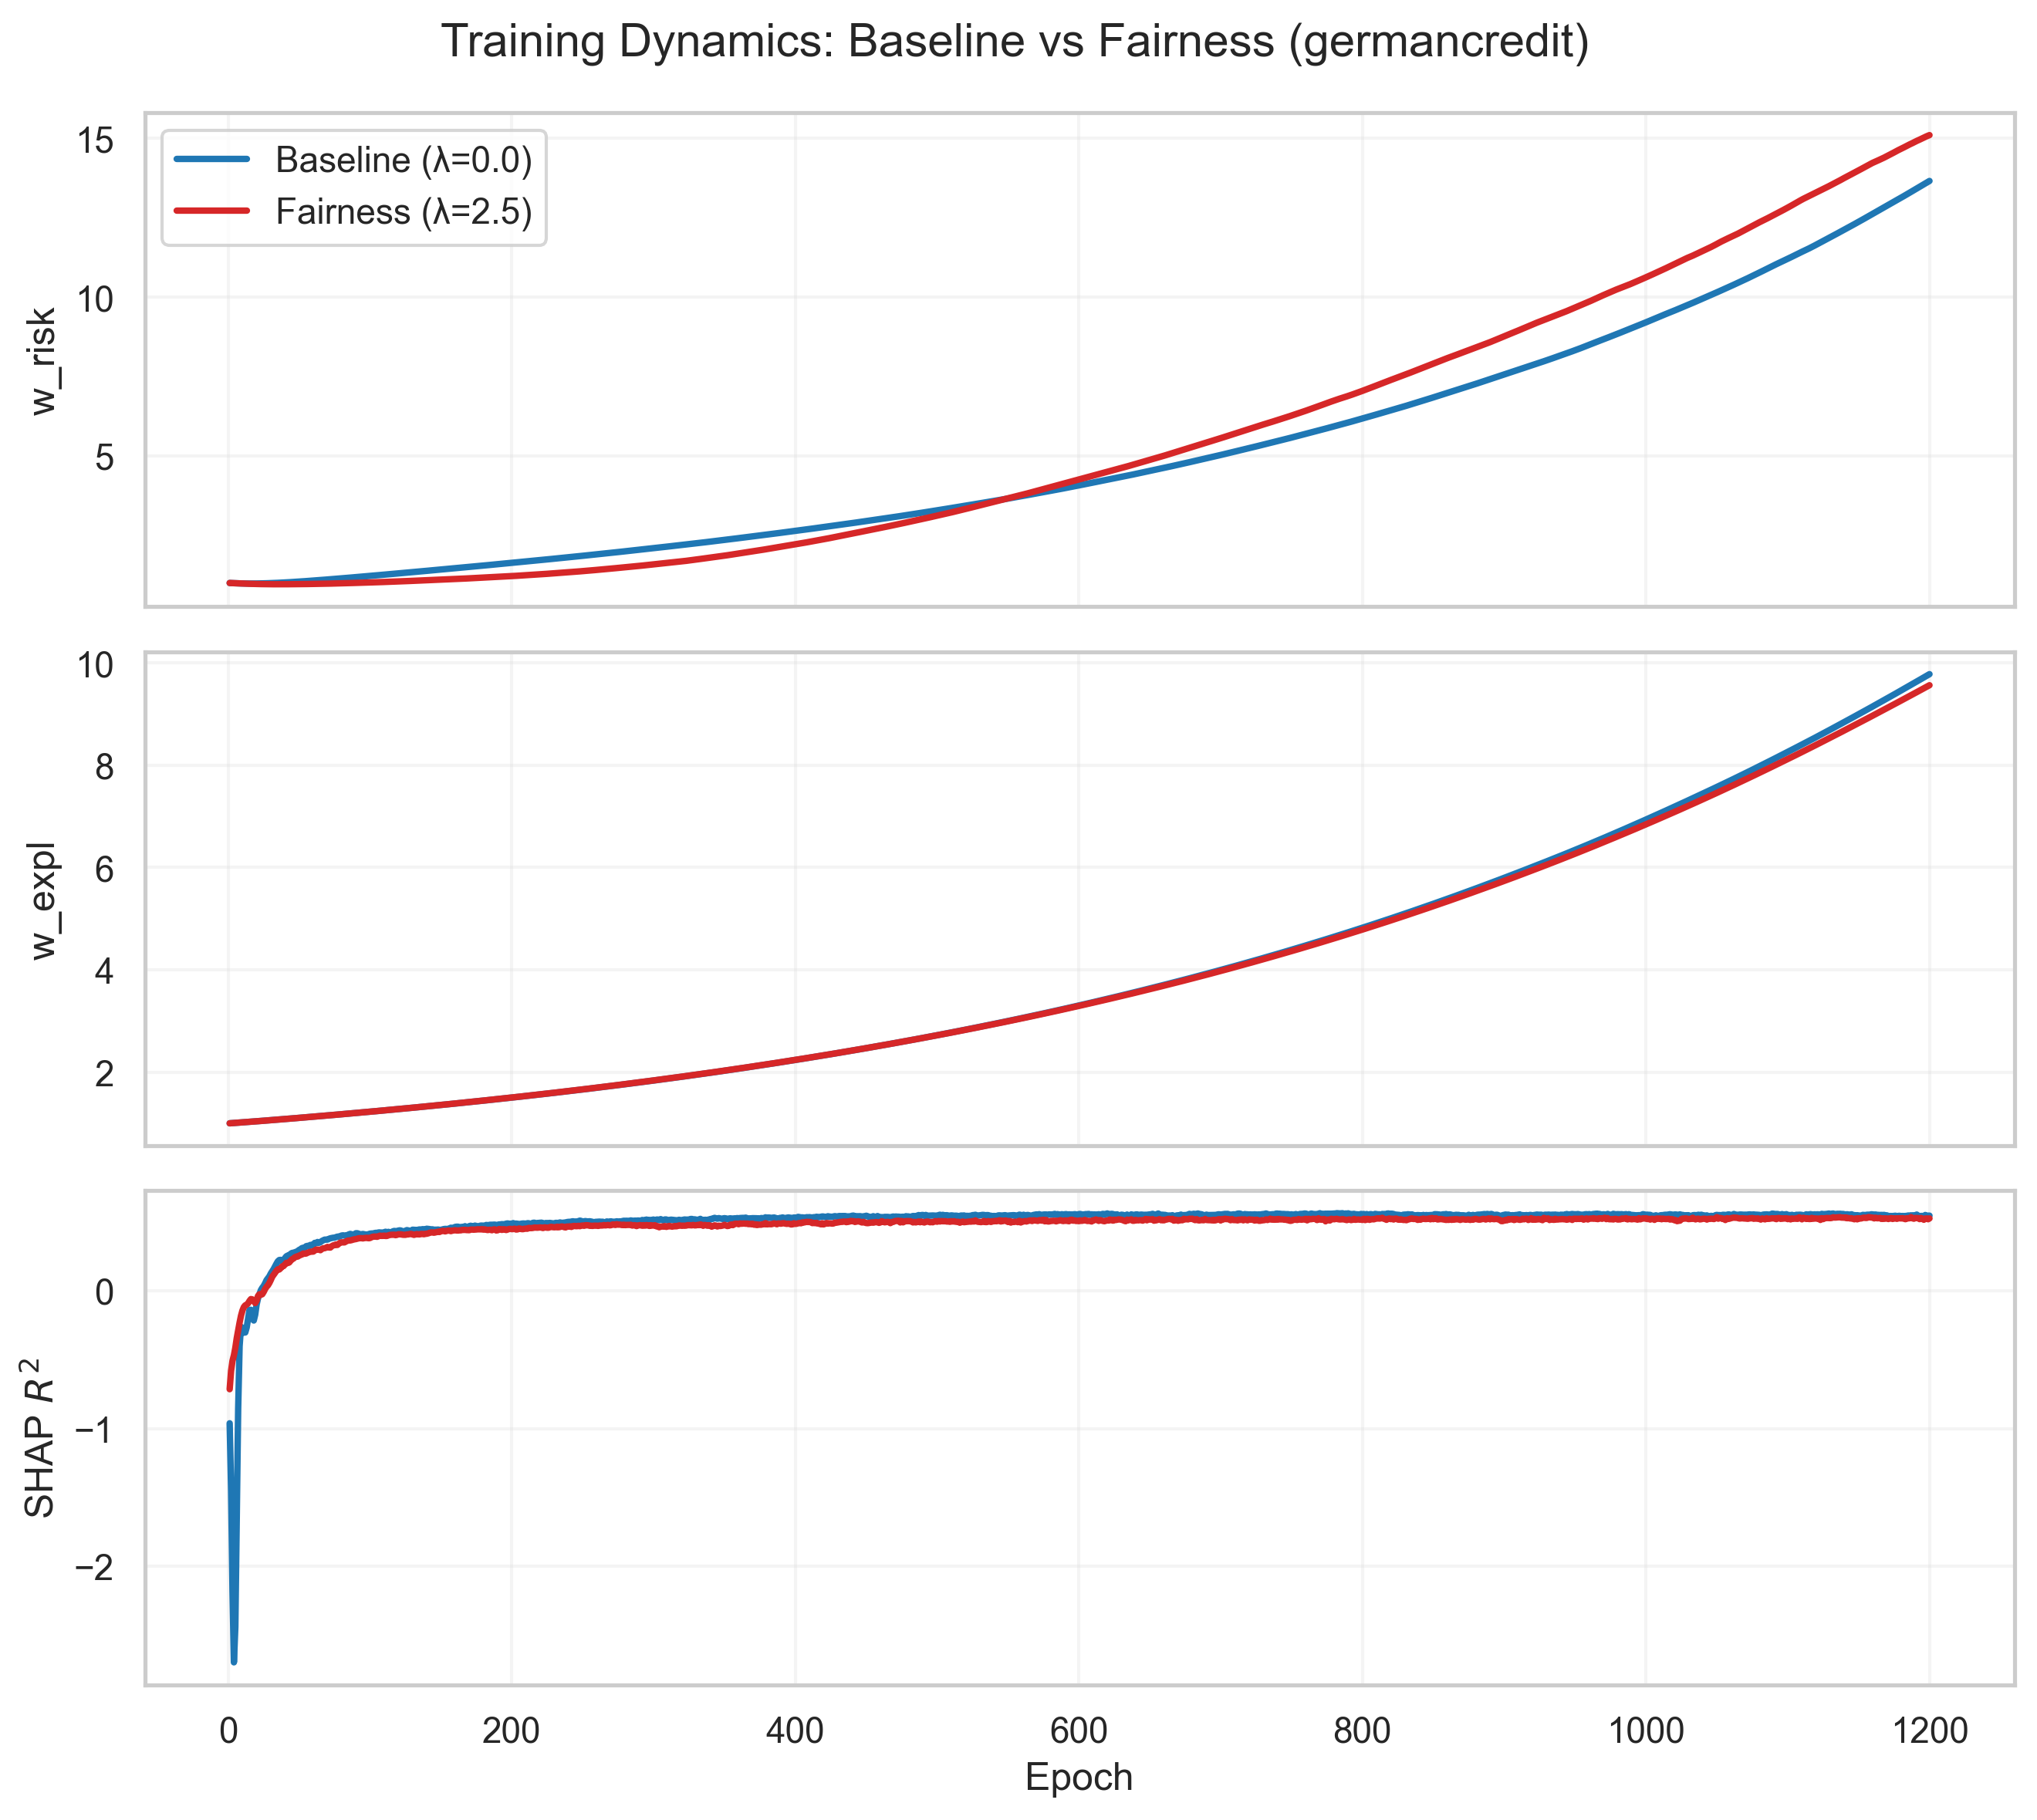
\includegraphics[width=0.32\columnwidth]{fig_wsc_eloi/fig_results_training_dynamics_germancredit.png}\hfill
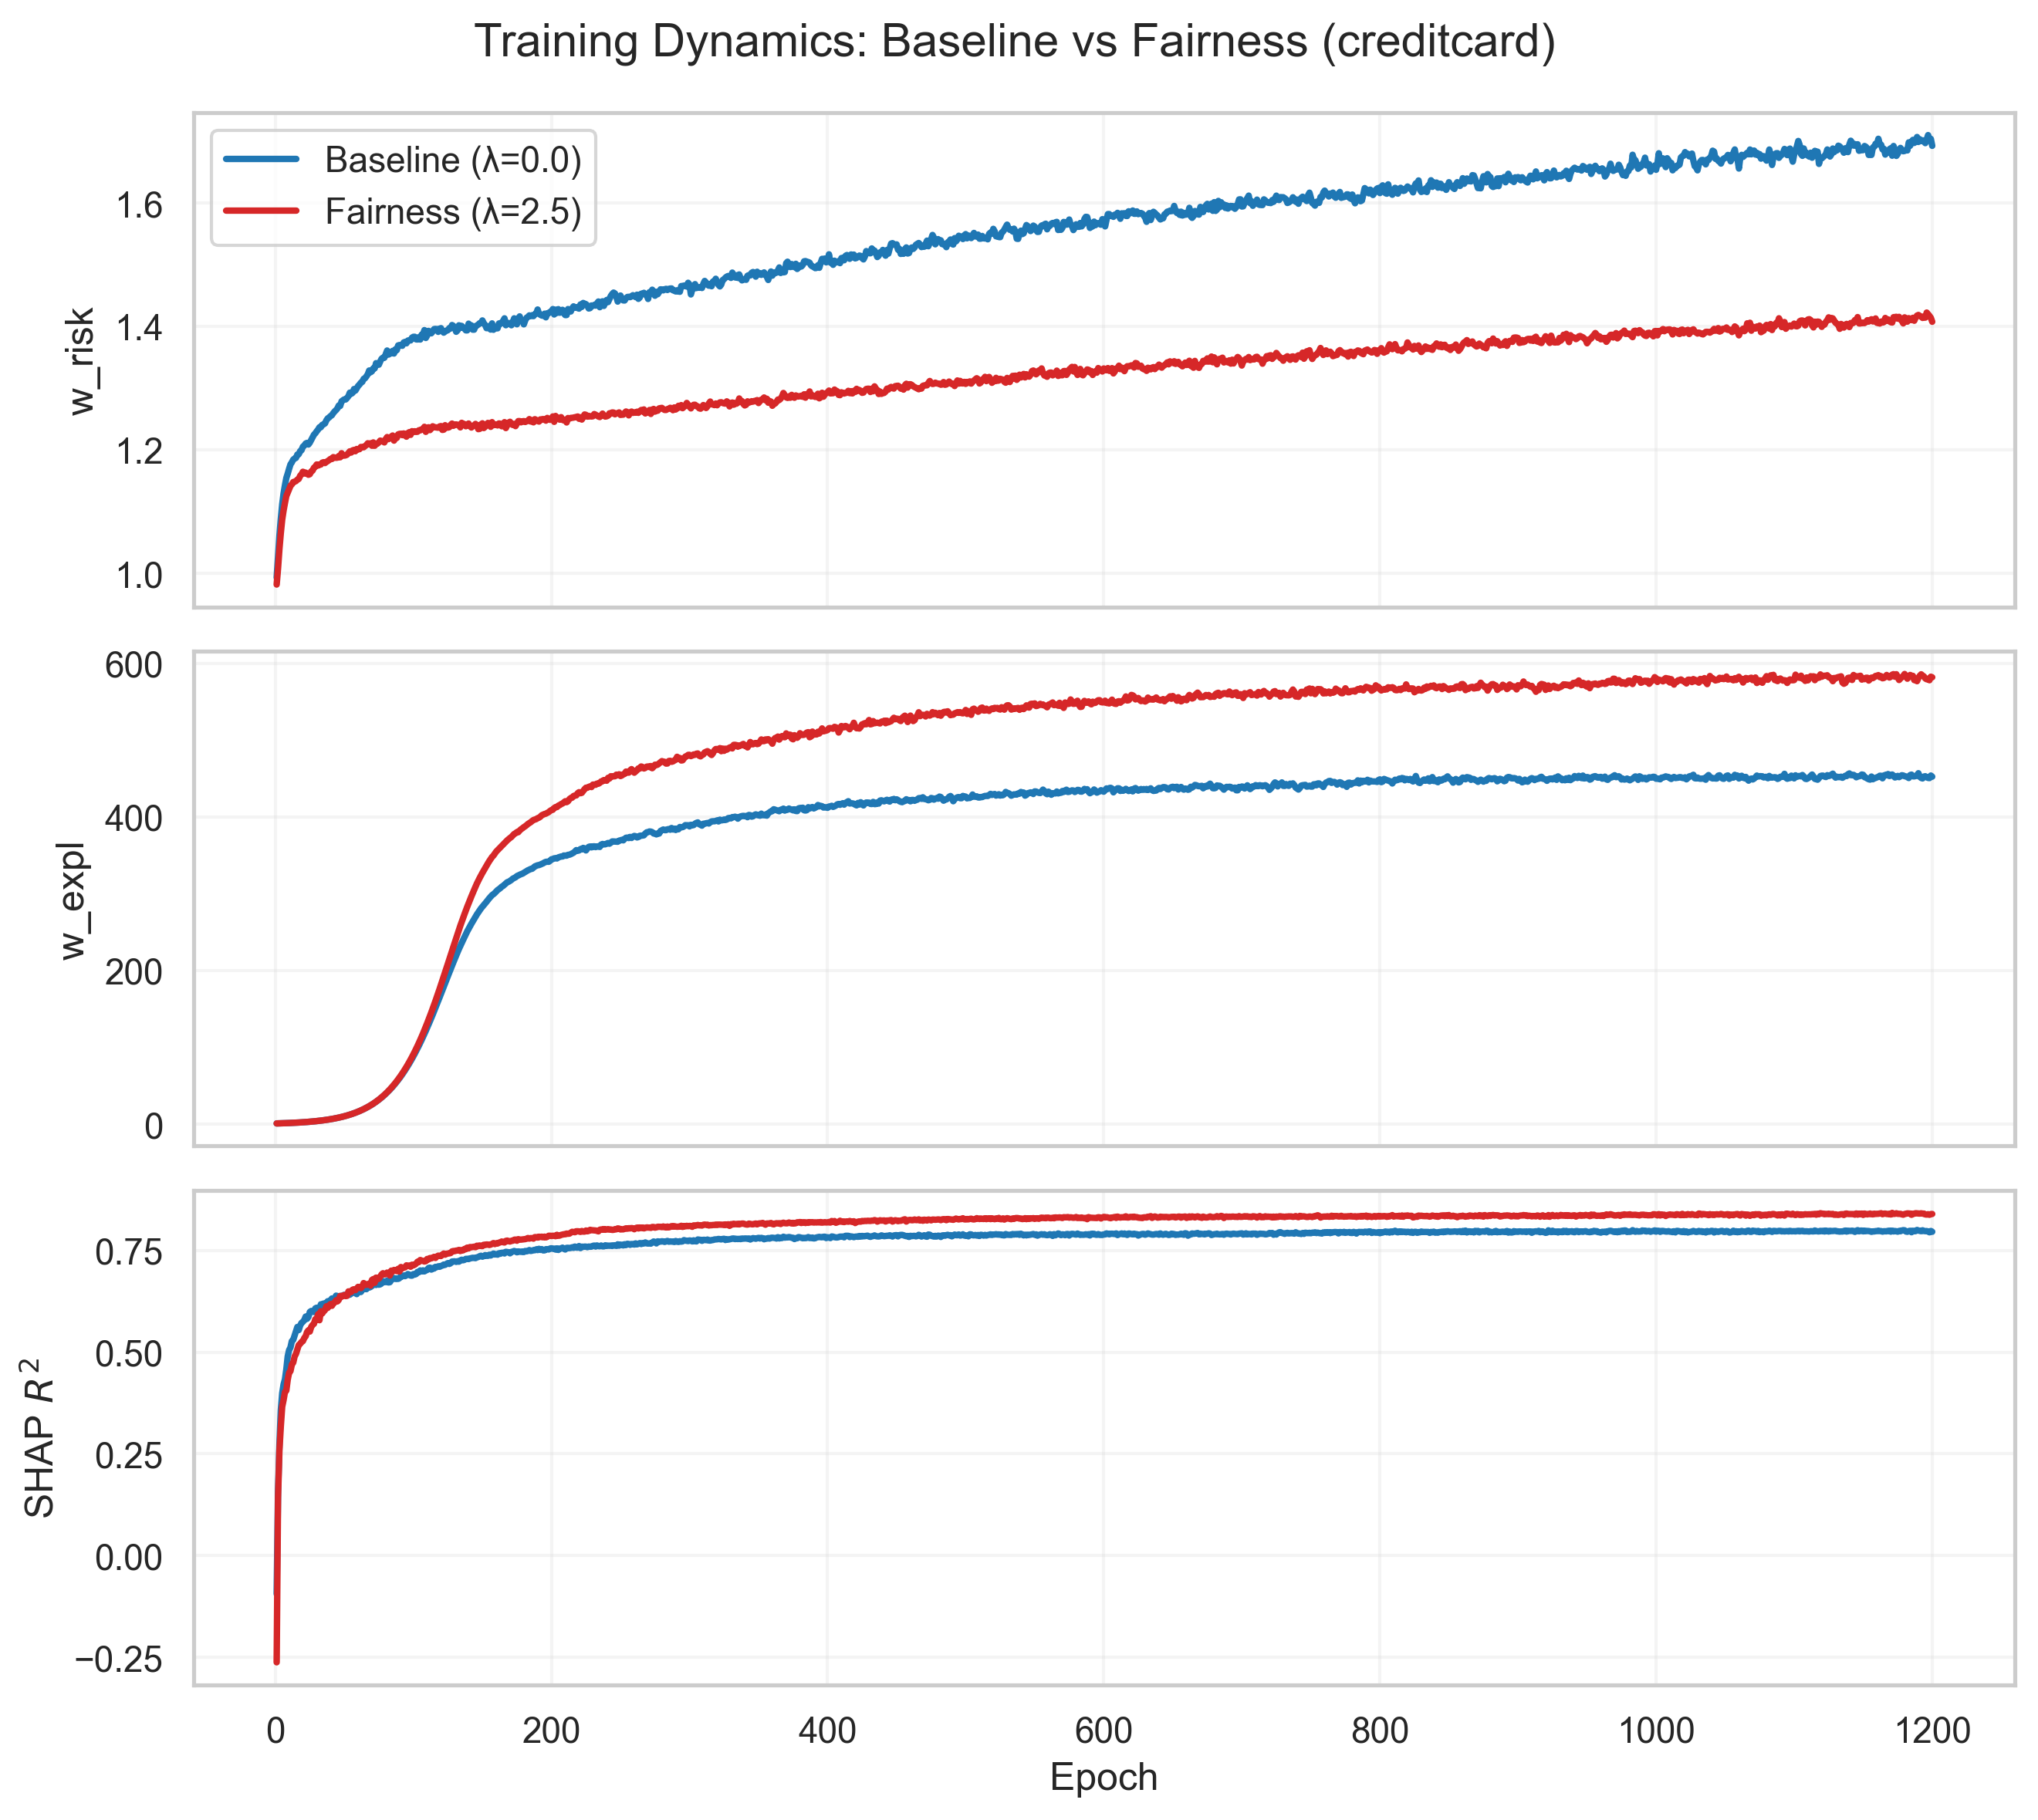
\includegraphics[width=0.32\columnwidth]{fig_wsc_eloi/fig_results_training_dynamics_creditcard.png}
\caption{Training dynamics under baseline vs fairness-constrained distillation across datasets: Bank Marketing (left), German Credit (center), and UCI Credit Card (right).}
\label{fig:training_dynamics_results}
\end{figure}

Overall, the distilled architecture preserves strong ranking quality, substantially narrows DP gaps, and provides real-time explainable scoring with large latency gains. Figure~\ref{fig:training_dynamics_results} further supports that optimization remains stable under fairness-constrained training.

\section{SCENARIO-BASED SIMULATION STUDY}
\label{sec:simulation}

To move beyond single training runs, we treat the distillation pipeline as the \emph{system under study} and analyze it with a designed simulation experiment \cite{bcnn:simulation}. A \emph{scenario} is one configuration of the controllable factors; a \emph{replication} is one execution under an independent random seed (governing data shuffling, mini-batch permutation, and weight initialization). We report each response as a mean with a 95\% confidence interval (Student-$t$). Seeds, the 80/20 split, the architecture, and the homoscedastic weighting are held at their published values so that the baseline scenario reproduces the corresponding row of Table~\ref{tab:main_results}.

\subsection{Factors, Responses, and Design}
We vary four factors that govern the teacher--student interaction: teacher capacity (\texttt{n\_estimators}$\in\{50,100,200\}$, \texttt{max\_depth}$\in\{3,4,6\}$); fairness pressure $\lambda_{fair}\in\{0,0.5,1,2.5,5\}$; mini-batch size $\in\{64,256,512,1024\}$; and protected-group prevalence, induced by synthetically resampling the protected group to $\{1,3,5,10\}\%$ of the Student's training set while holding the Teacher and its TreeSHAP targets fixed. Responses are AUC, SHAP $R^2$, the demographic-parity (DP) gap, the Equal-Opportunity (EO) and Equalized-Odds (EOdds) gaps (Section~\ref{sec:eo}), training stability (mean/maximum global gradient norm, a divergence flag, and the fraction of mini-batches masked by the safety net), and P99 latency. We use a one-factor-at-a-time design over all factors plus a $4\times4$ full-factorial on the two most operationally relevant factors ($\lambda_{fair}\times$ prevalence). German Credit uses the full grid (five seeds); UCI Credit Card and Bank Marketing use a focused grid (three seeds, reduced epochs) reporting trends.

\subsection{Fairness Pressure and the Accuracy/Fairness Frontier}
Table~\ref{tab:lambda_sweep} summarizes the $\lambda_{fair}$ sweep. Three regimes appear, organized by protected-group prevalence. For the well-balanced UCI Credit Card group ($46.9\%$) the penalty is near-ideal: the DP gap falls monotonically ($0.037\!\to\!0.013$) with AUC statistically flat ($0.767$ across $\lambda$). For the imbalanced Bank Marketing group ($2.7\%$) the trilemma genuinely binds: the DP gap collapses ($0.325\!\to\!0.035$) but AUC declines significantly ($0.926\!\to\!0.897$). For the tiny German Credit group (31 training instances) the penalty is unreliable---the DP gap is non-monotone and rises at large $\lambda$ ($0.114\!\to\!0.188$)---because $25.6\%$ of mini-batches trip the safety net and the surviving in-batch estimates are high-variance. Crucially, in no dataset does fairness pressure \emph{improve} AUC; the effect is neutral or costly (Figure~\ref{fig:sim_lambda}).

\begin{table}[htb]
\centering
\caption{Fairness-pressure sweep: mean (95\% CI) over replications. German Credit: 5 seeds, full budget; UCI Credit Card / Bank Marketing: 3 seeds, reduced epochs (trends). Lower DP/EO gaps are better.}
\label{tab:lambda_sweep}
\footnotesize
\begin{tabular}{llccc}
\hline
Dataset & $\lambda_{fair}$ & AUC & DP gap & EO gap \\ \hline
German Credit    & 0.0 & 0.800 (0.016) & 0.114 & 0.400 \\
German Credit    & 2.5 & 0.792 (0.007) & 0.157 & 0.505 \\
German Credit    & 5.0 & 0.786 (0.012) & 0.188 & 0.475 \\ \hline
UCI Credit Card  & 0.0 & 0.767 (0.004) & 0.037 & 0.076 \\
UCI Credit Card  & 2.5 & 0.768 (0.002) & 0.026 & 0.052 \\
UCI Credit Card  & 5.0 & 0.767 (0.003) & 0.013 & 0.022 \\ \hline
Bank Marketing   & 0.0 & 0.926 (0.004) & 0.325 & 0.118 \\
Bank Marketing   & 2.5 & 0.905 (0.002) & 0.059 & 0.342 \\
Bank Marketing   & 5.0 & 0.897 (0.004) & 0.035 & 0.221 \\ \hline
\end{tabular}
\end{table}

\begin{figure}[htb]
\centering
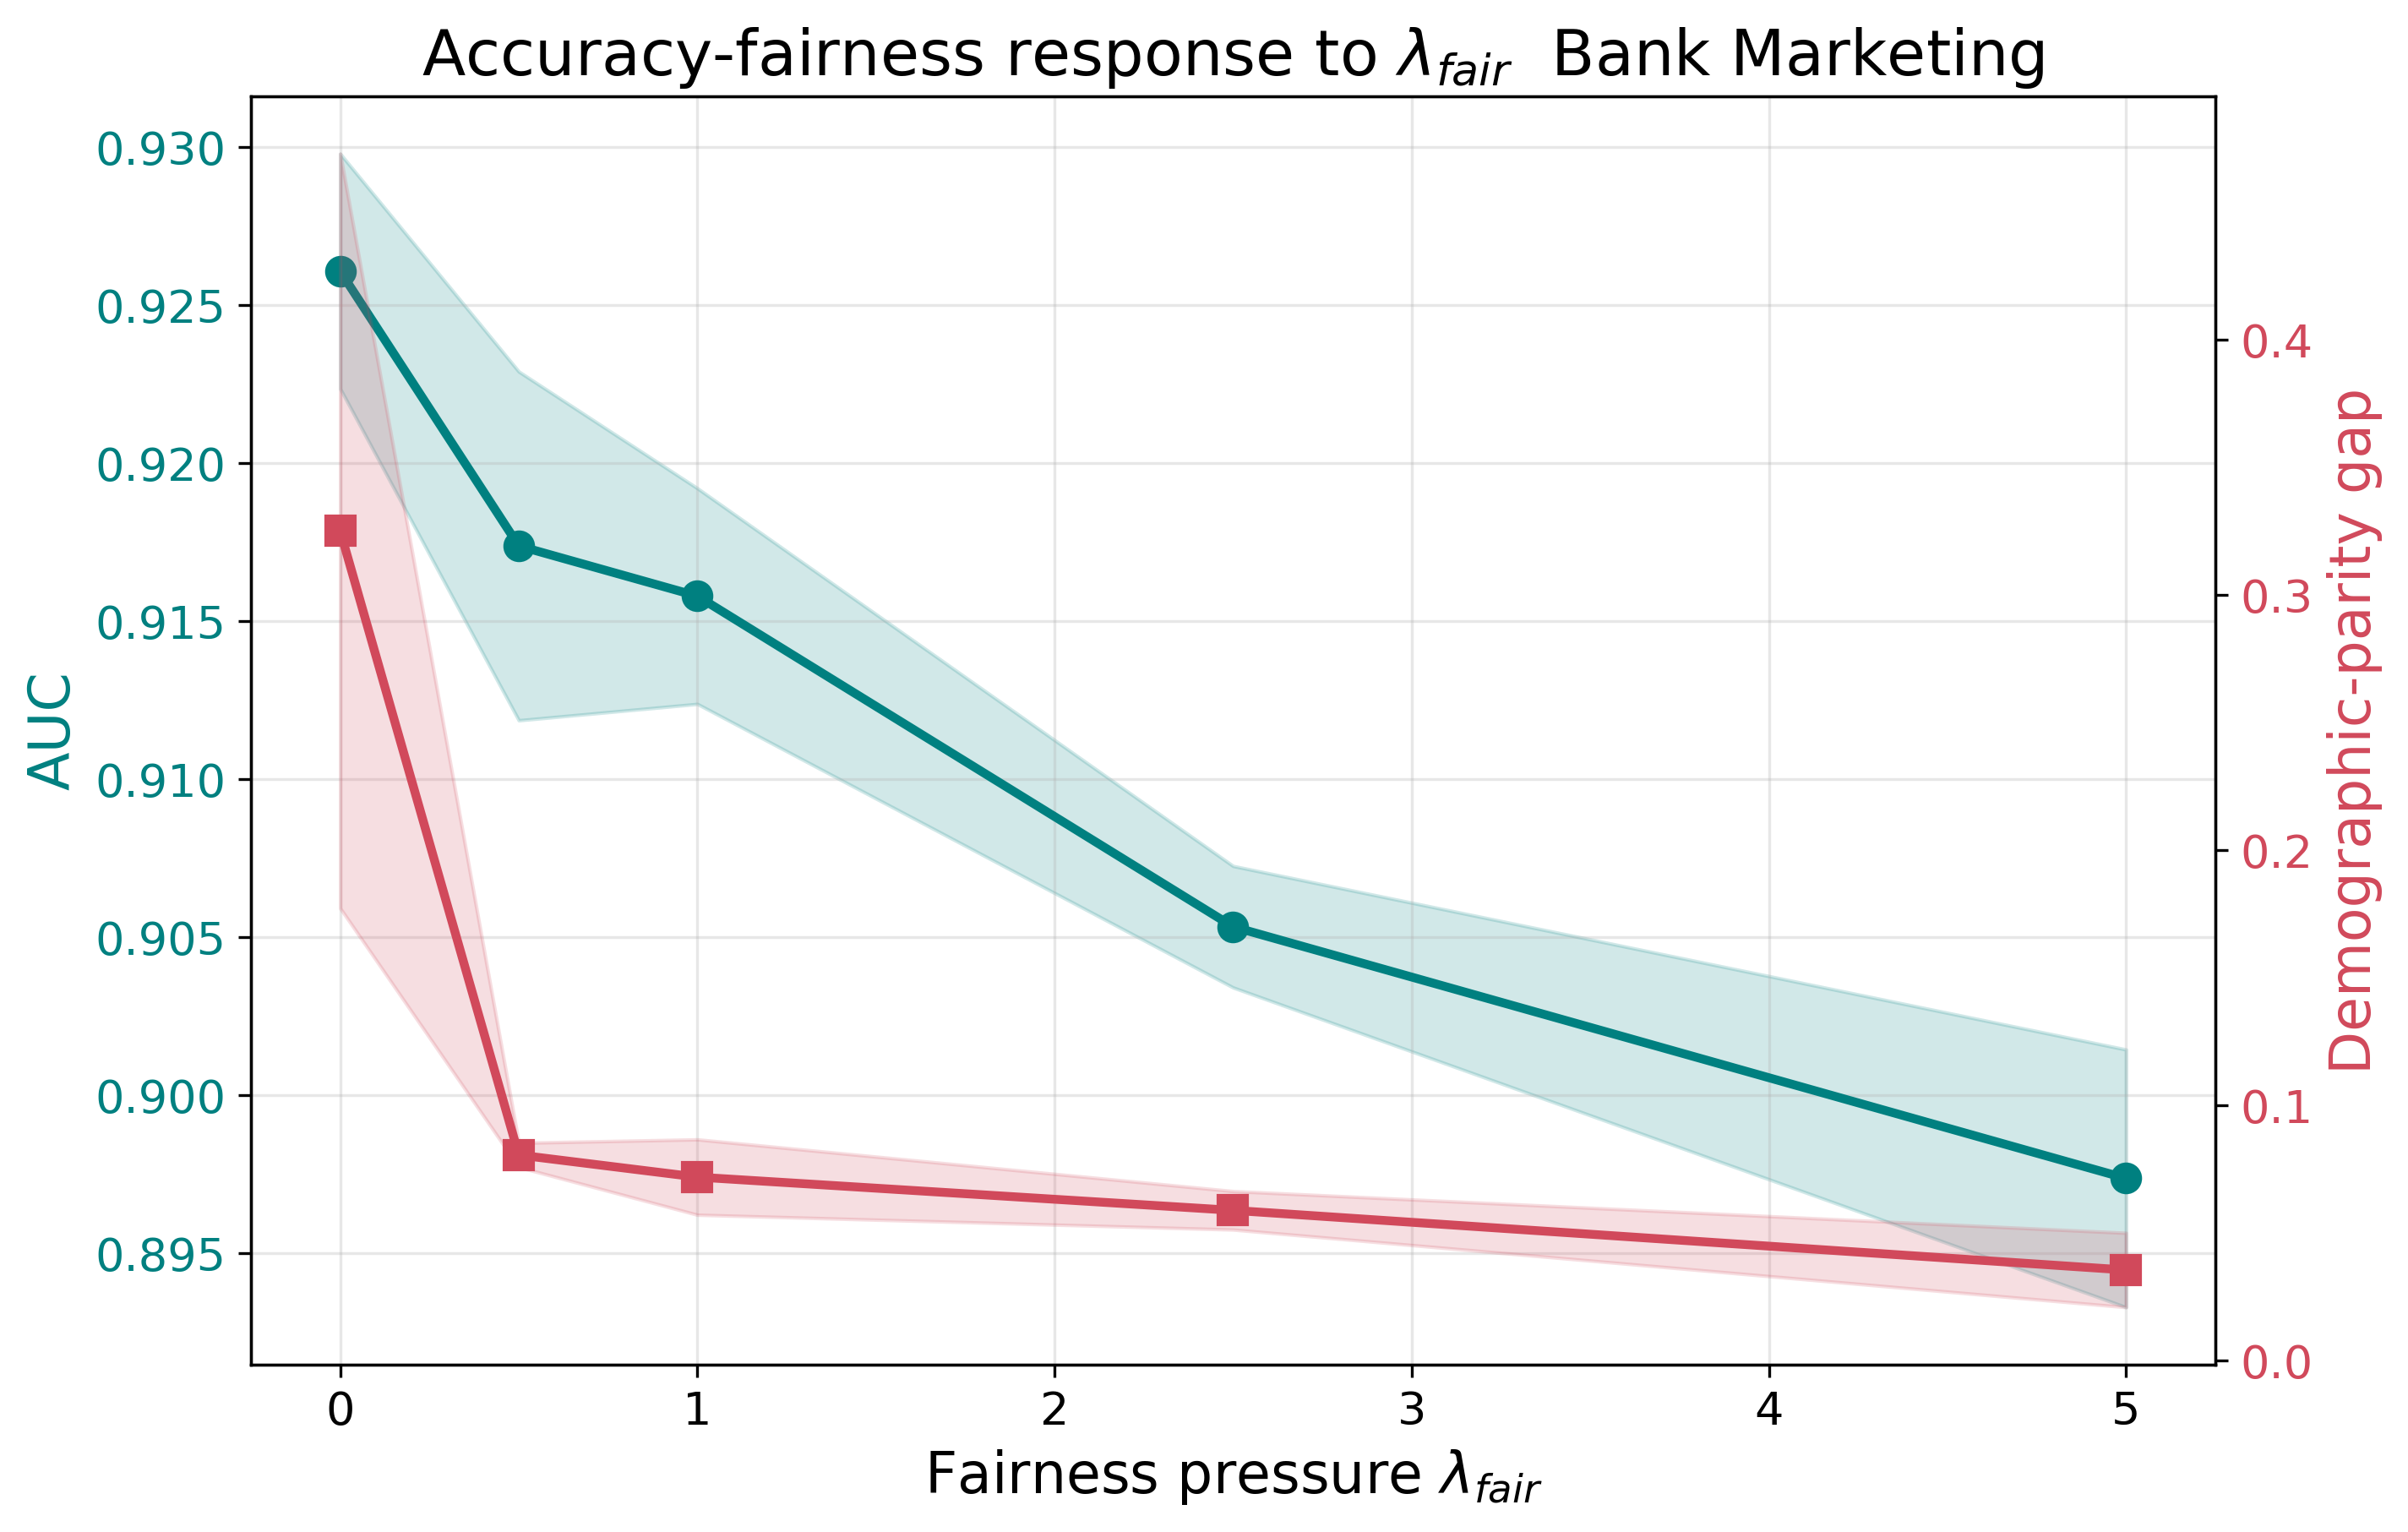
\includegraphics[width=0.32\columnwidth]{fig_wsc_eloi/fig_sim_lambda_bankmarketing.png}\hfill
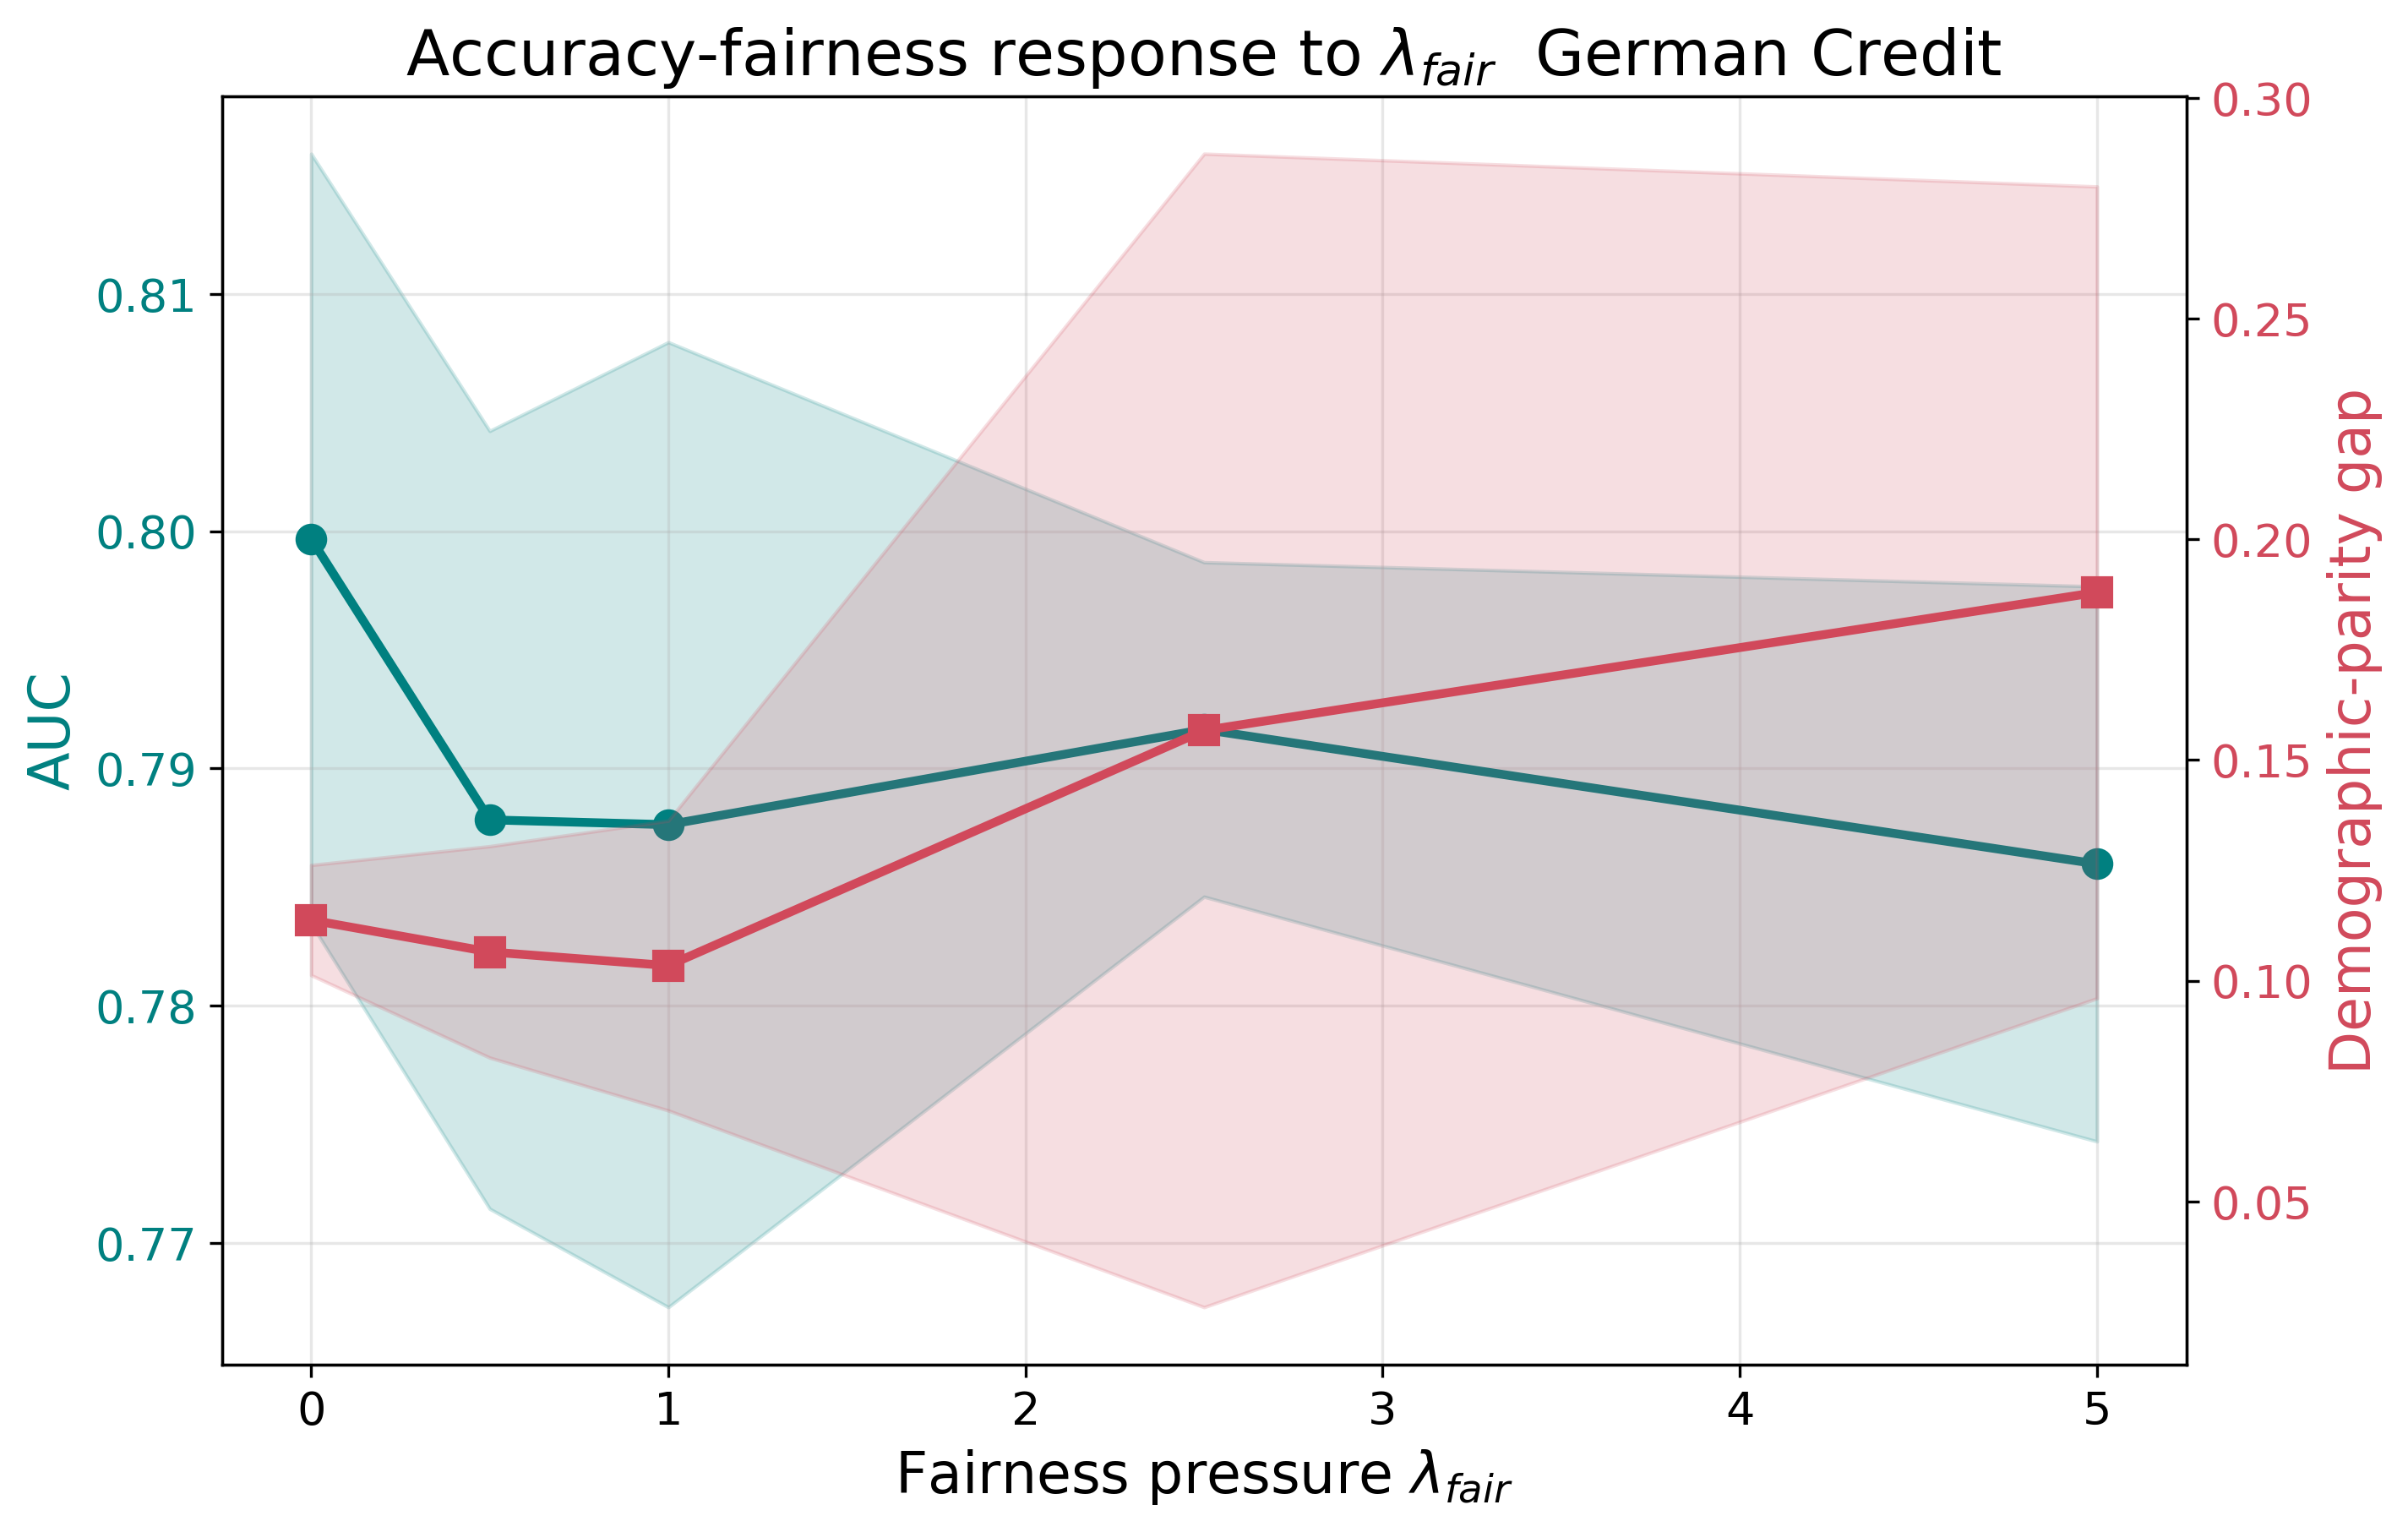
\includegraphics[width=0.32\columnwidth]{fig_wsc_eloi/fig_sim_lambda_germancredit.png}\hfill
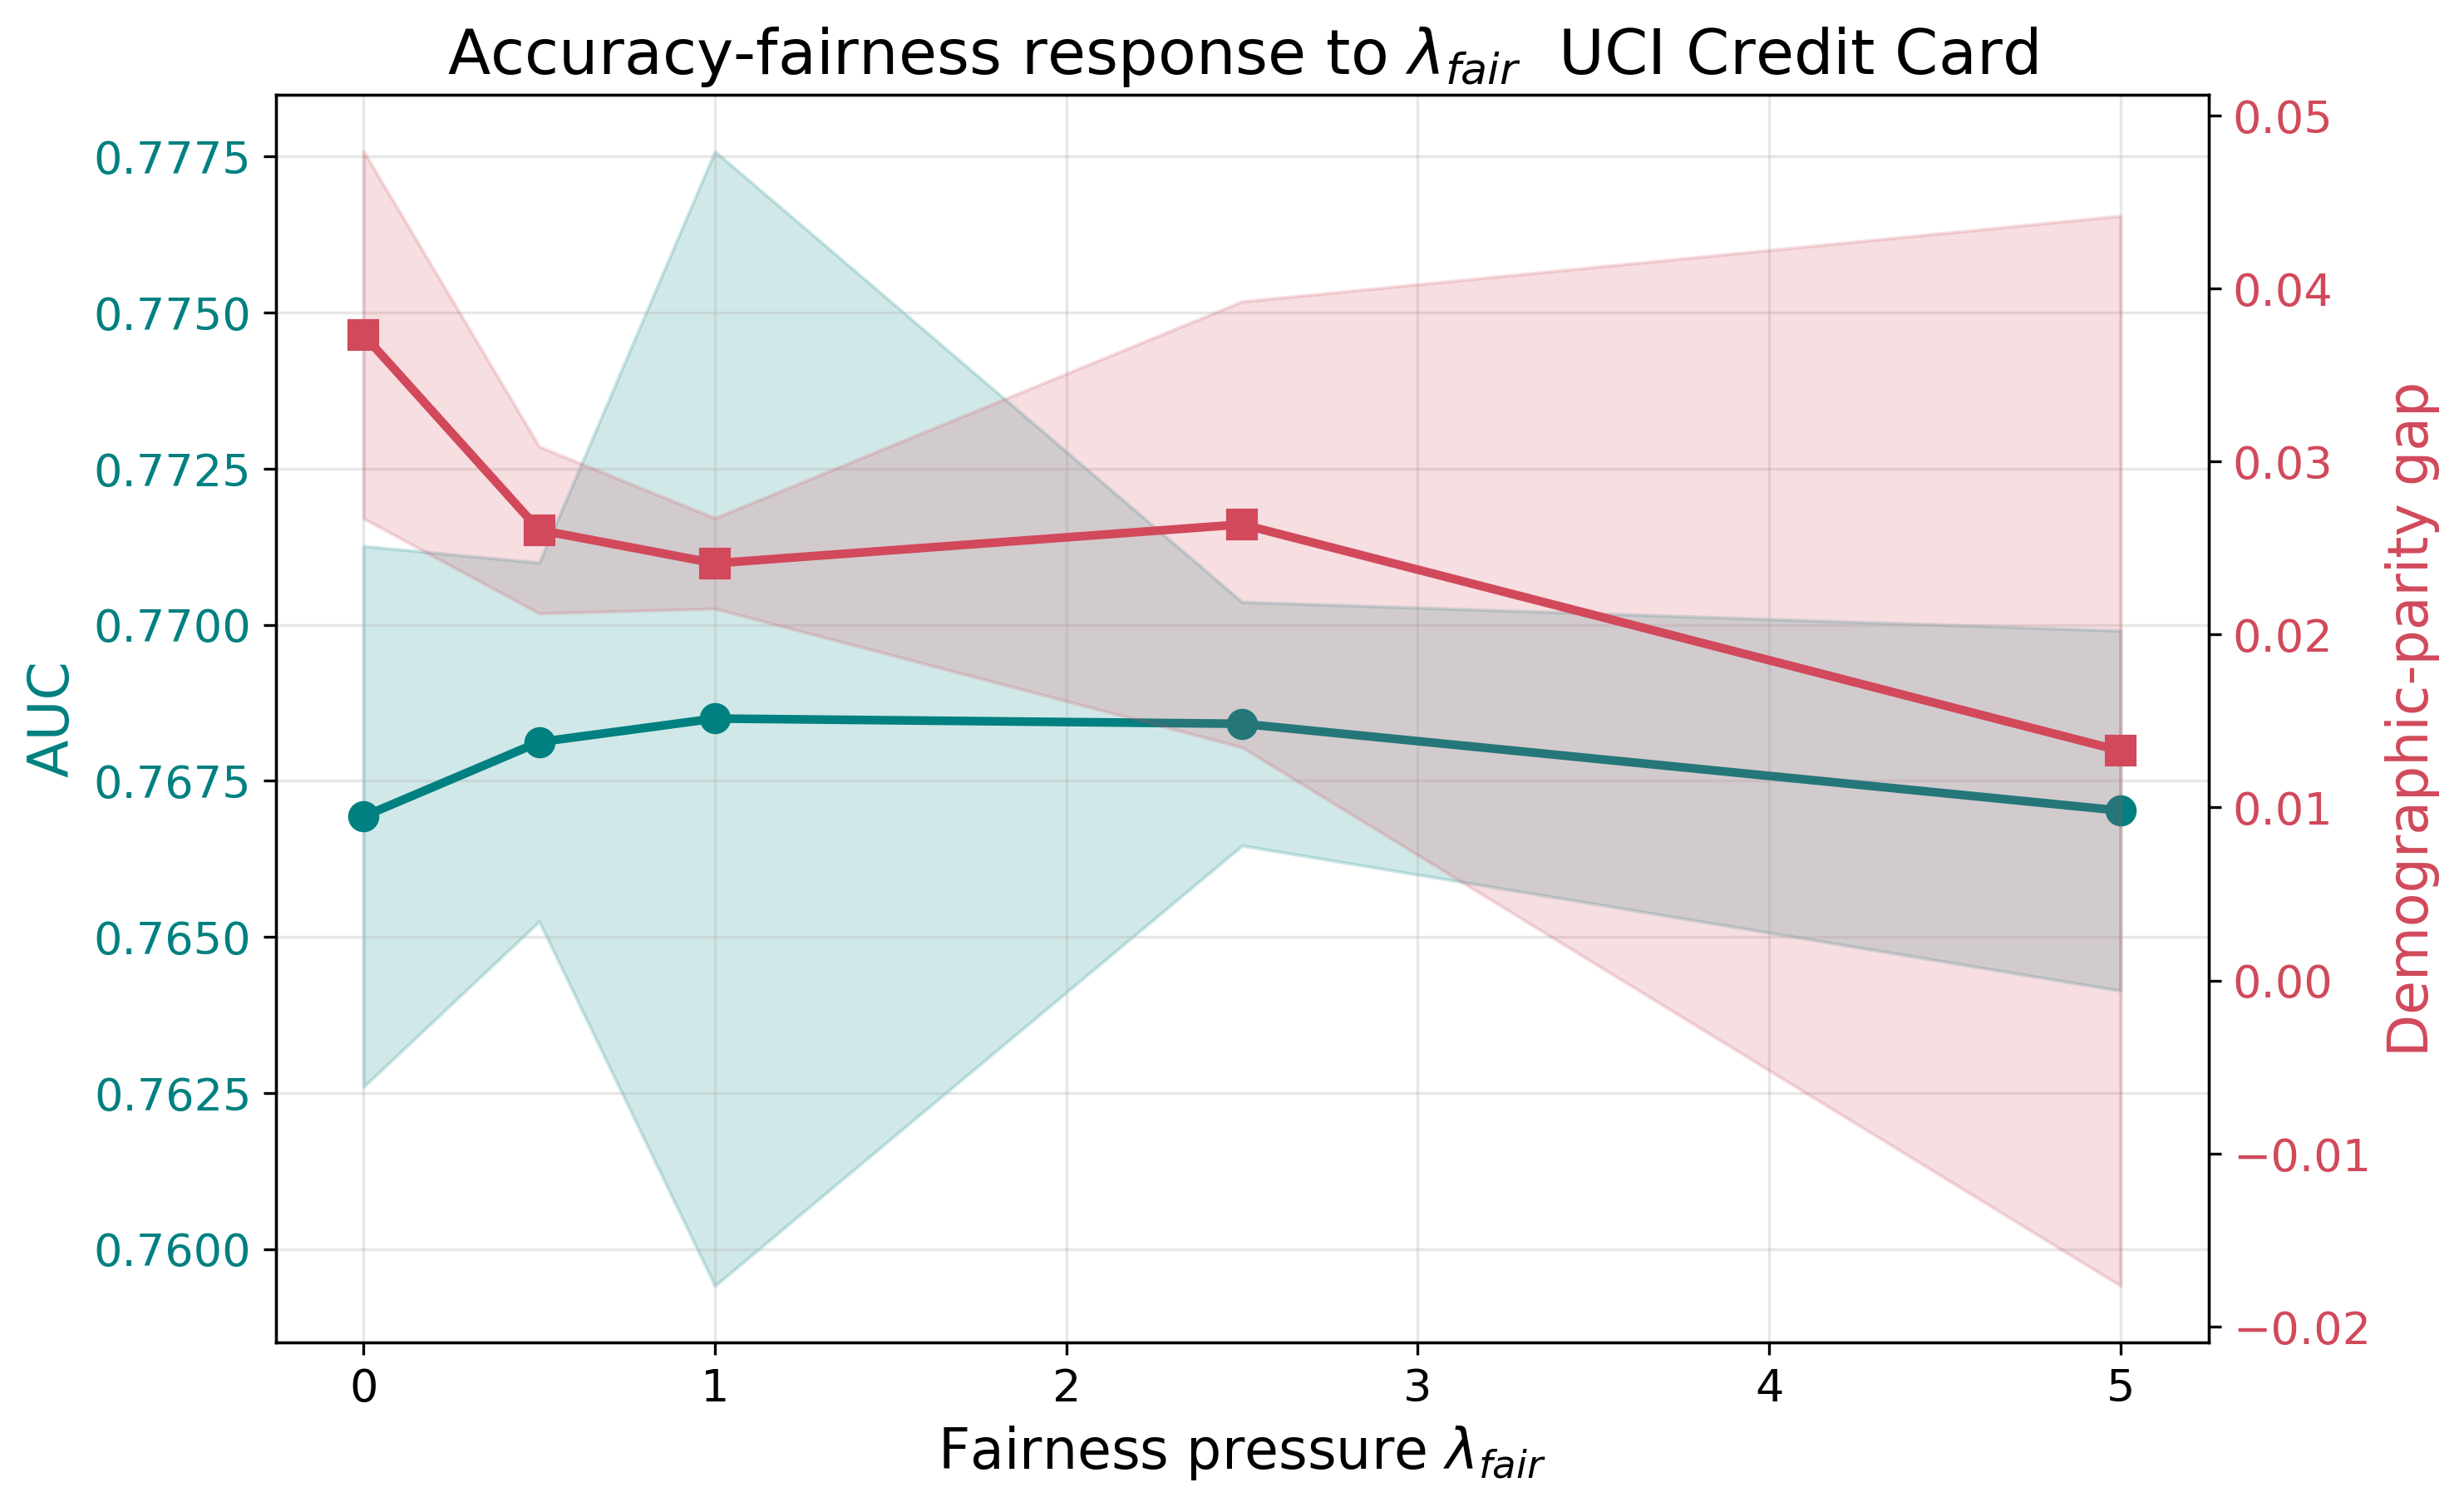
\includegraphics[width=0.32\columnwidth]{fig_wsc_eloi/fig_sim_lambda_creditcard.png}
\caption{Accuracy--fairness response to $\lambda_{fair}$ with 95\% CI bands (AUC, left axis; DP gap, right axis): Bank Marketing (left), German Credit (center), UCI Credit Card (right). Bank Marketing shows a clear trade-off; UCI Credit Card removes bias at no accuracy cost.}
\label{fig:sim_lambda}
\end{figure}

\subsection{Training Stability: Batch Size and Protected-Group Prevalence}
The simulation confirms that stability is governed by the statistical resolution of the in-batch fairness signal. On German Credit, shrinking the protected group $10\%\!\to\!1\%$ raises the safety-net-masked fraction $1.1\%\!\to\!93.6\%$ and the maximum gradient norm $11.8\!\to\!47.2$; shrinking the batch size $1024\!\to\!64$ raises the masked fraction $0\%\!\to\!91.5\%$ and the maximum gradient norm $1.8\!\to\!154.8$ (Figure~\ref{fig:sim_stability}). Bank Marketing reproduces the batch-size pattern (batch 64 masks $97\%$ with gradient norm $68$). No configuration diverged (no non-finite loss across all runs), supporting the claim that the large-batch protocol and safety net prevent the instability they target. Teacher capacity raises the Student's SHAP $R^2$ ($0.42\!\to\!0.48$ as \texttt{n\_estimators} $50\!\to\!200$ on German Credit) while leaving the label-supervised risk head's AUC flat---consistent with the clarification in Section~\ref{sec:results}.

\begin{figure}[htb]
\centering
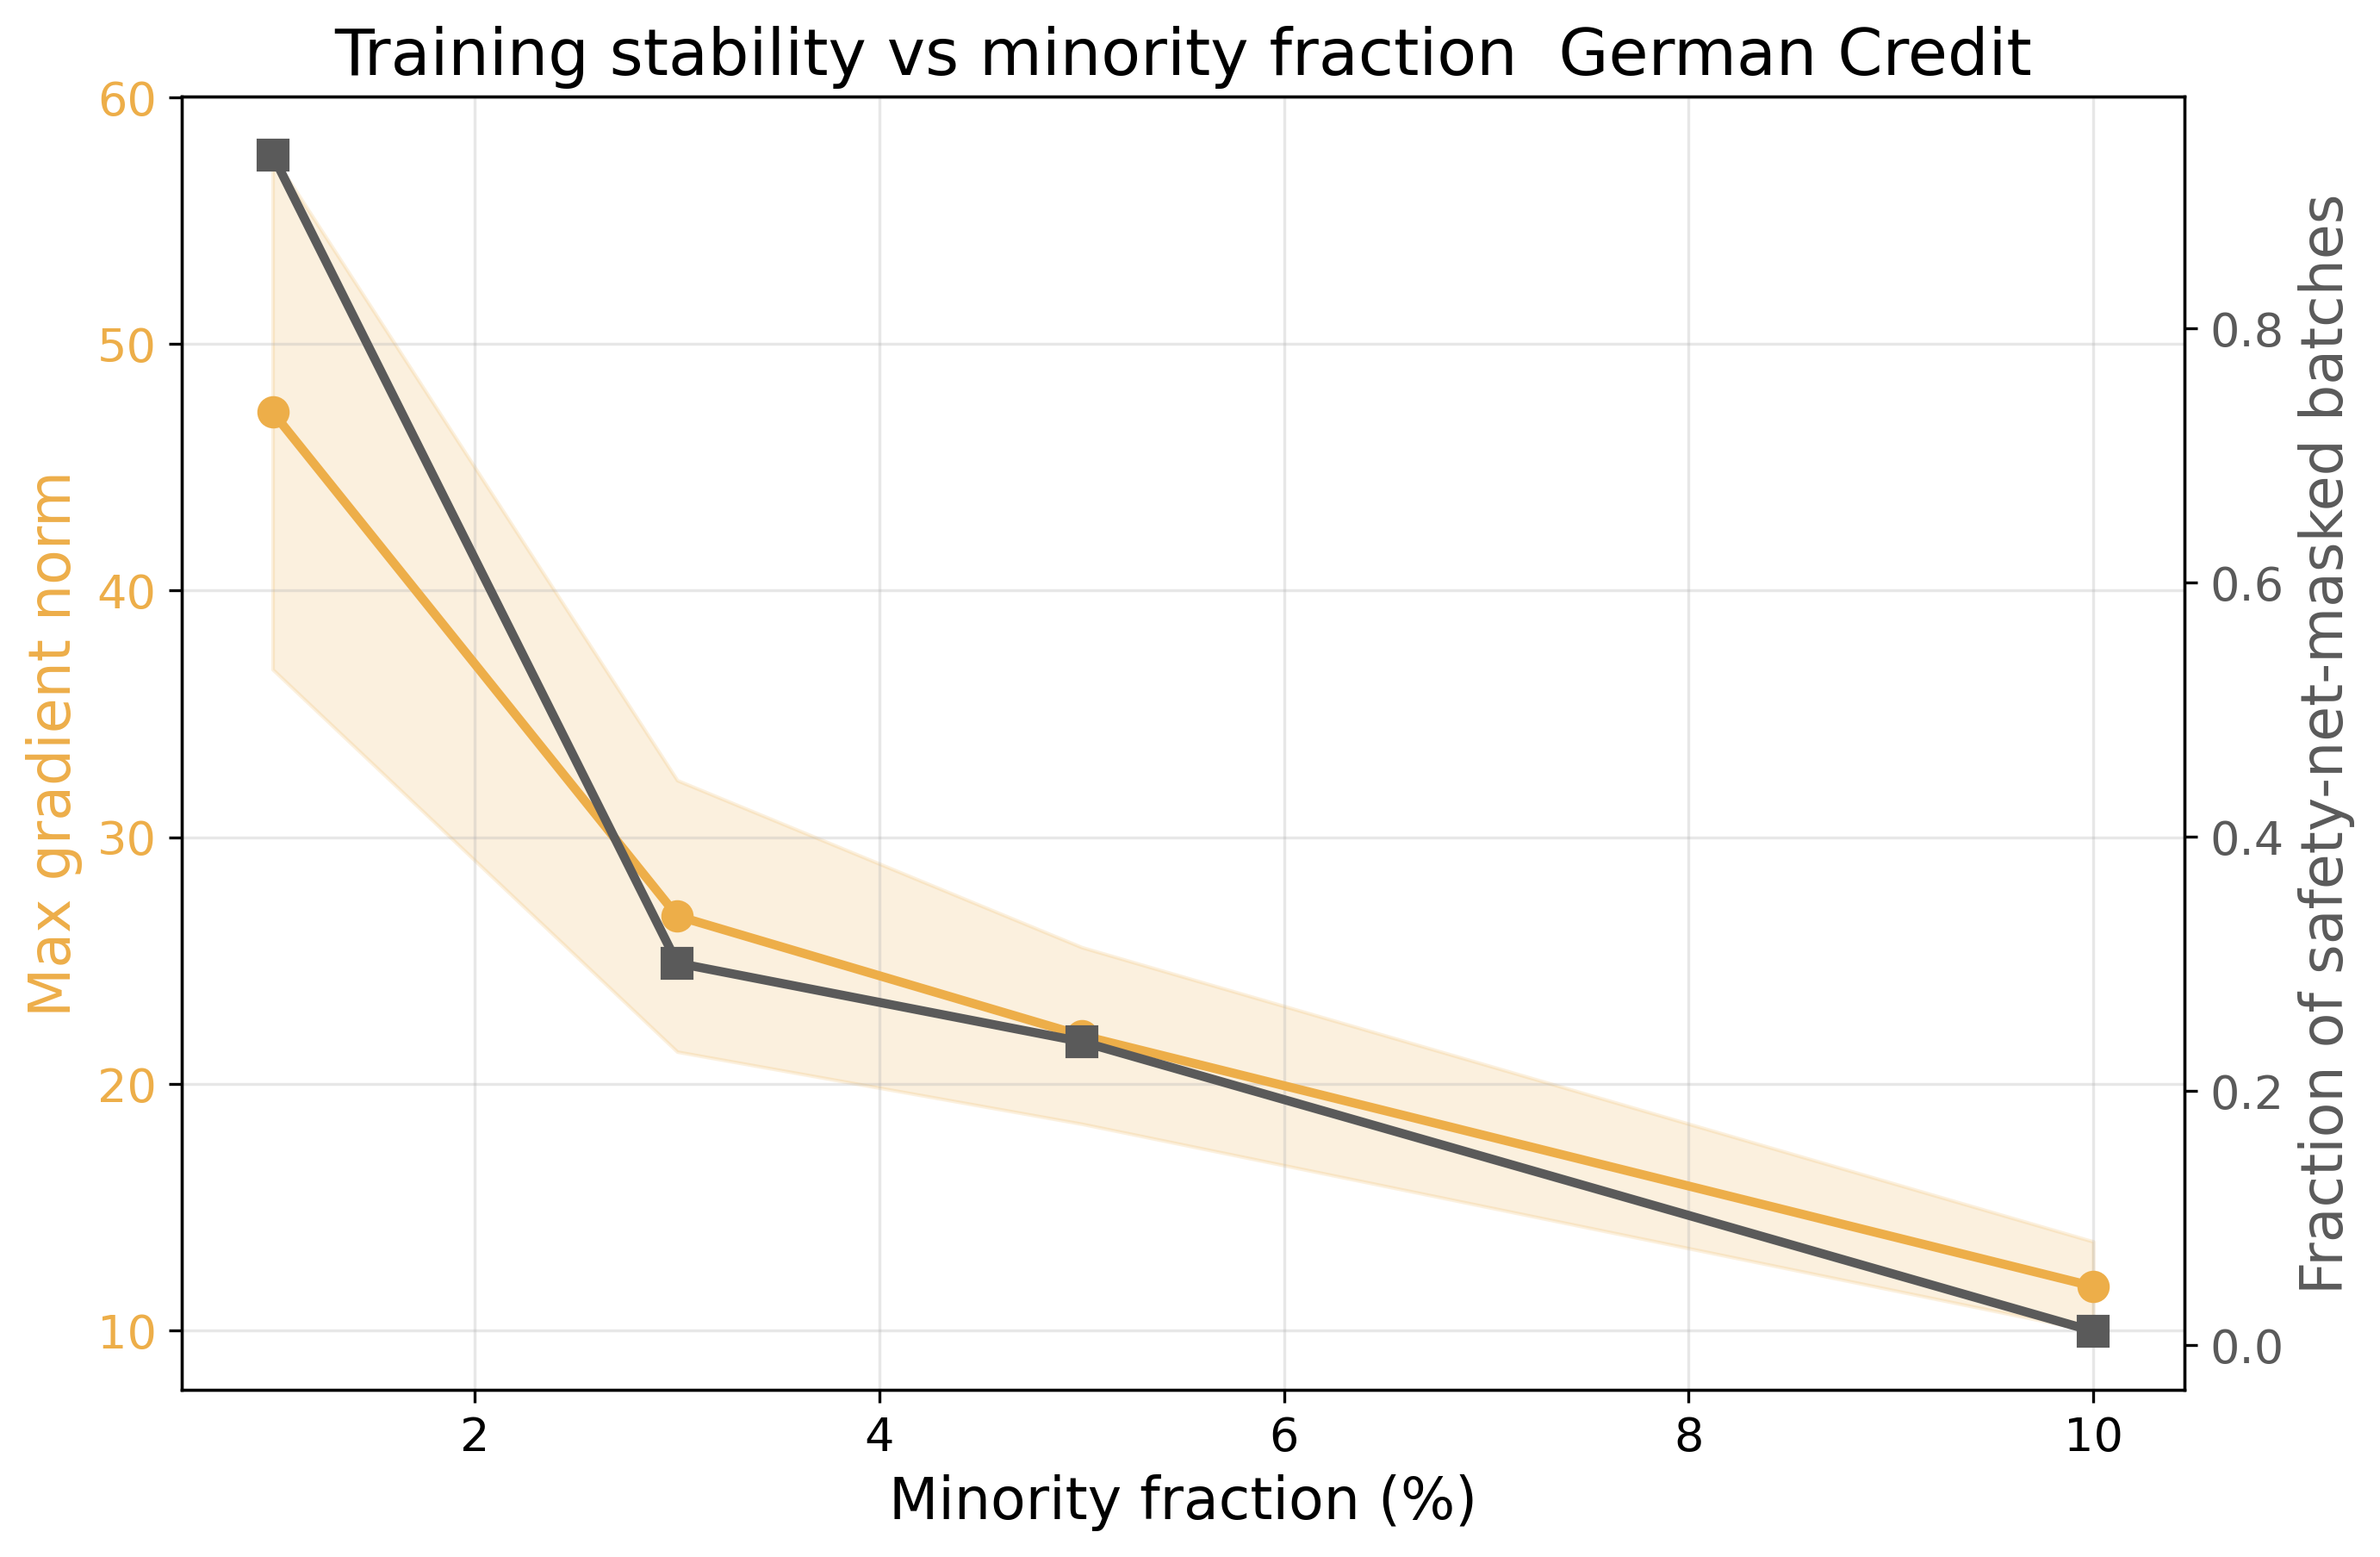
\includegraphics[width=0.42\columnwidth]{fig_wsc_eloi/fig_sim_stability_germancredit.png}\hfill
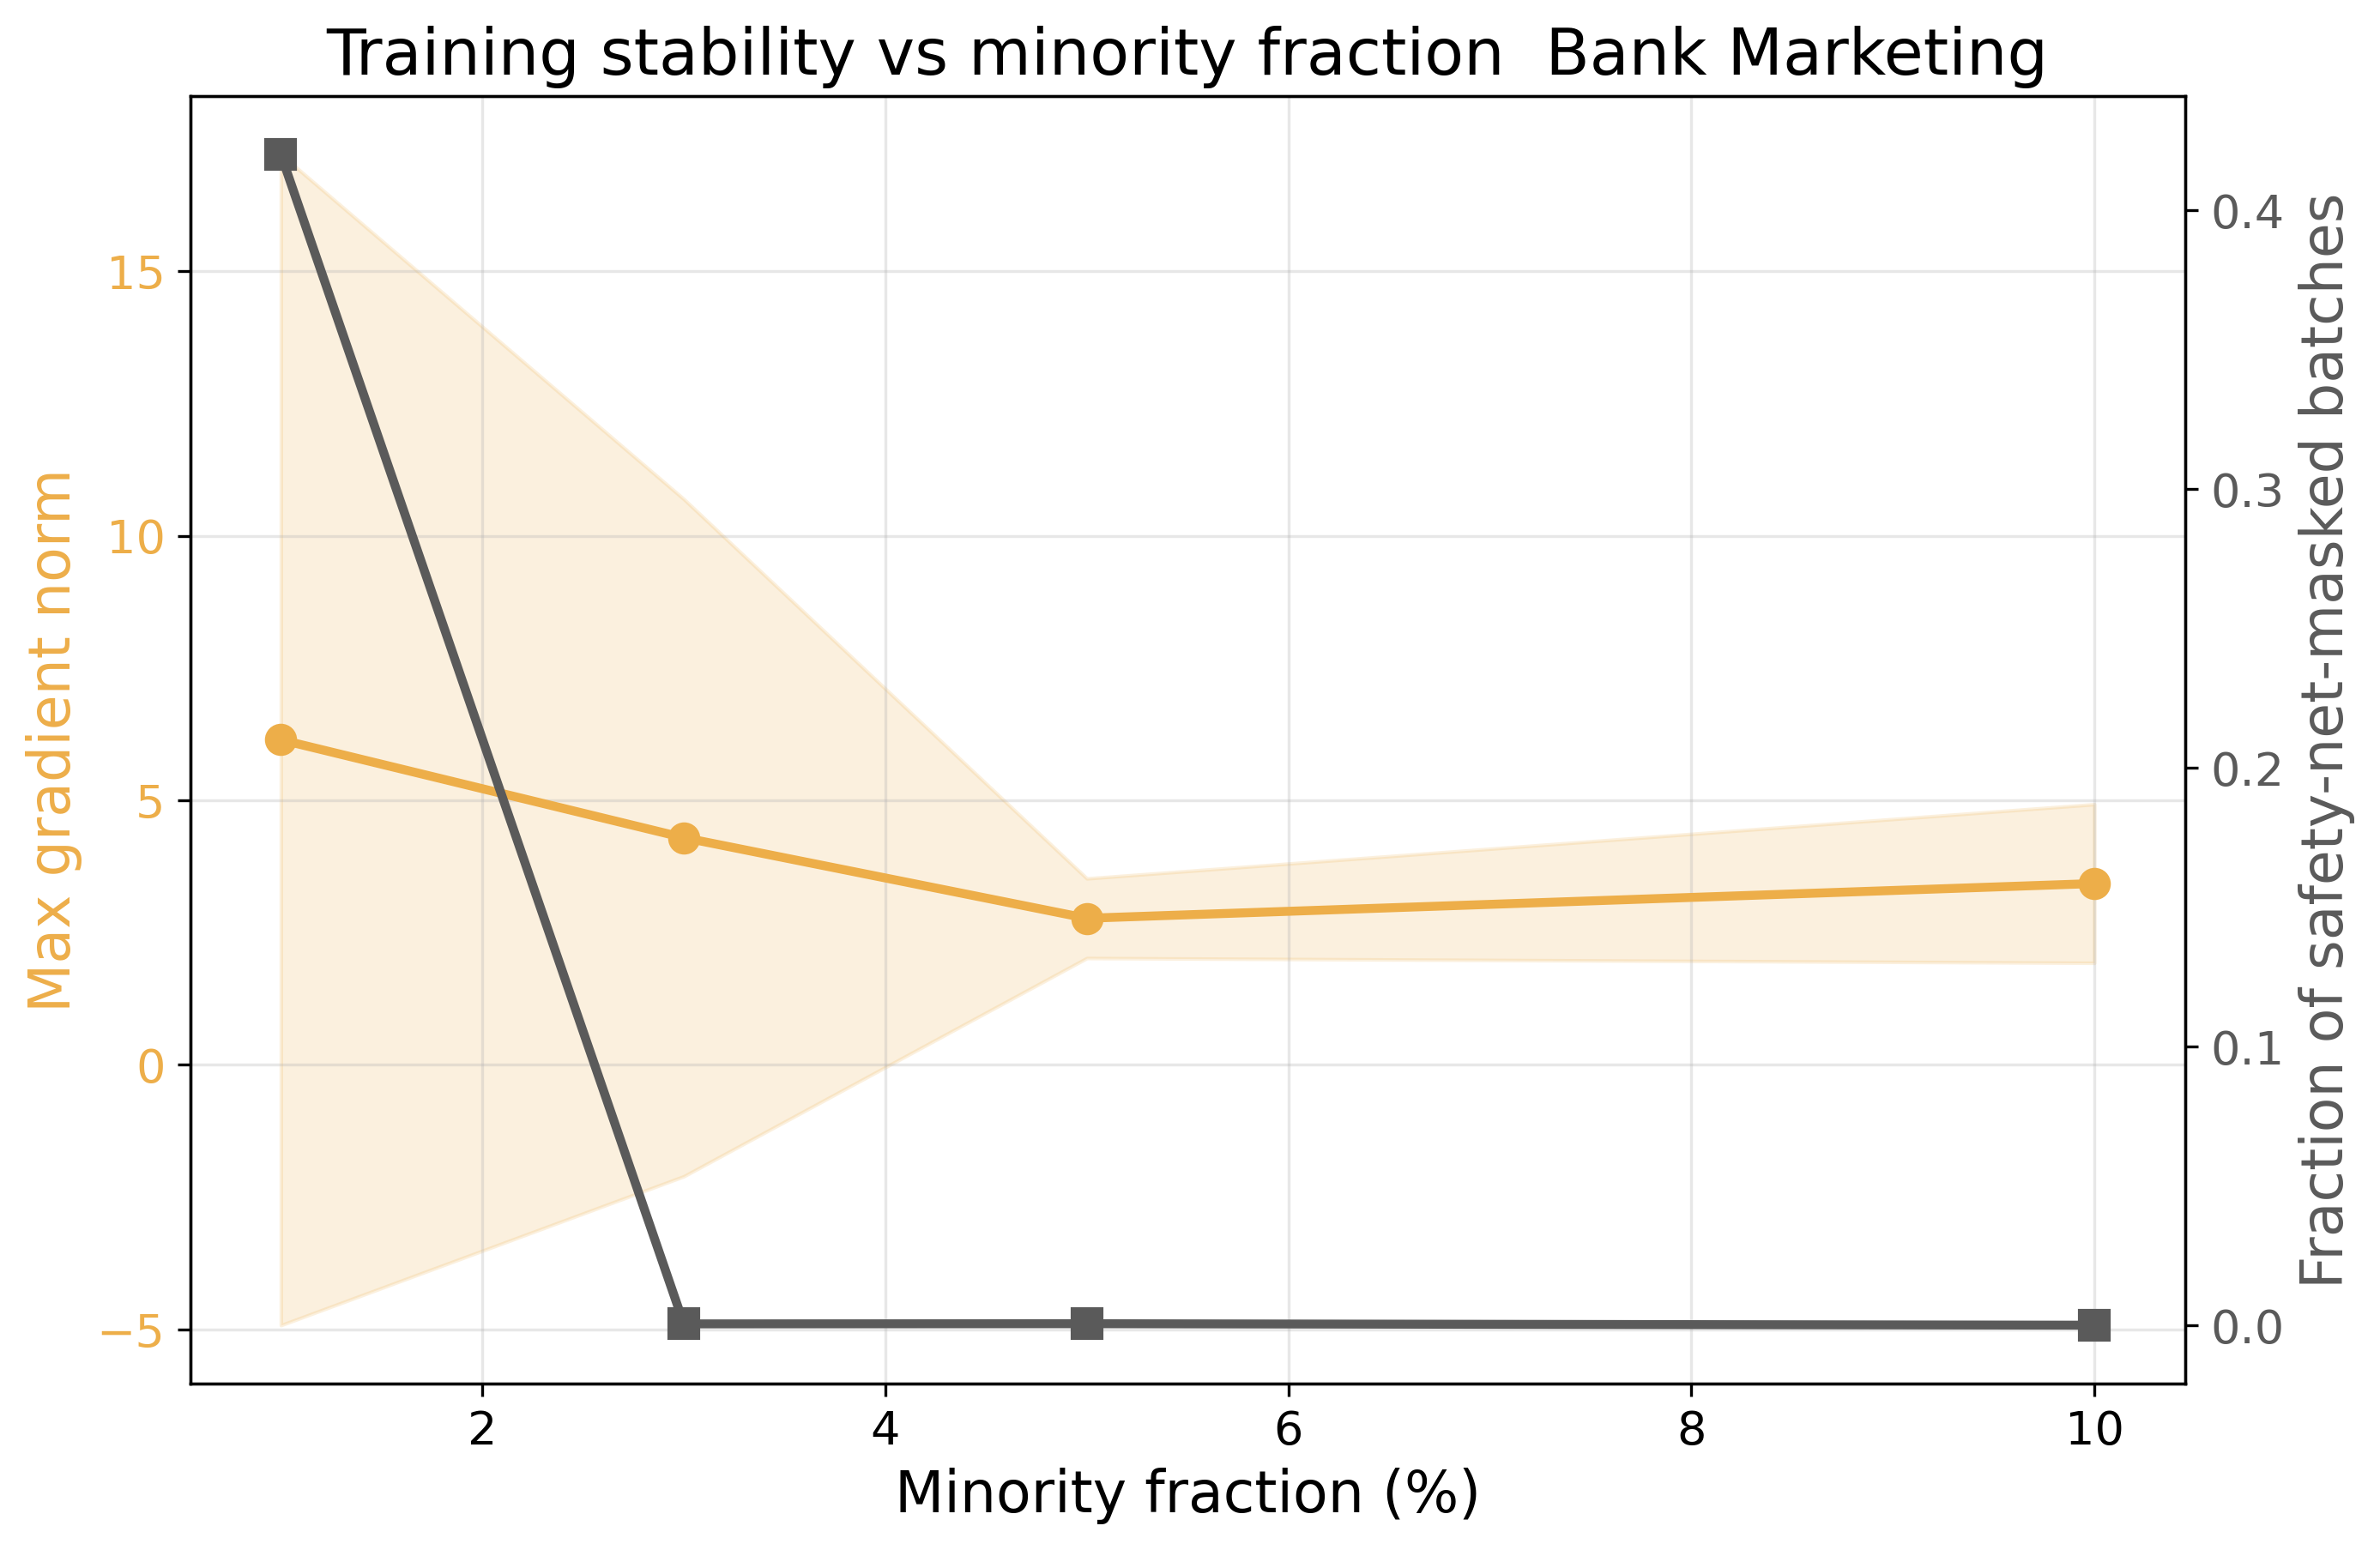
\includegraphics[width=0.42\columnwidth]{fig_wsc_eloi/fig_sim_stability_bankmarketing.png}
\caption{Training stability vs.\ protected-group prevalence: maximum gradient norm and safety-net-masked batch fraction (95\% CI). German Credit (left), Bank Marketing (right). Scarcer groups trigger more masking and larger gradients, yet training never diverges.}
\label{fig:sim_stability}
\end{figure}

\subsection{Beyond Demographic Parity: Equal Opportunity and Equalized Odds}
\label{sec:eo}
The submitted work measured fairness only as a DP gap \cite{Dwork2012Fairness}, which ignores the ground-truth label. We add two label-conditioned criteria \cite{Hardt2016Equality}: Equal Opportunity, $|\mathrm{TPR}_{A=1}-\mathrm{TPR}_{A=0}|$ (conditioned on $y=1$), and Equalized Odds, $\max(|\Delta\mathrm{TPR}|,|\Delta\mathrm{FPR}|)$. Both are computed for all models. The decisive evidence is on Bank Marketing: as $\lambda_{fair}$ rises the DP-targeted penalty drives the DP gap down ($0.325\!\to\!0.035$) yet the EO gap moves in the \emph{opposite} direction, from $0.118$ at $\lambda{=}0$ to $0.49$ at $\lambda{=}0.5$ and remaining elevated (Table~\ref{tab:lambda_sweep}). Equalizing overall positive rates thus skews the true-positive rates across groups---DP and EO objectives conflict in the imbalanced regime. On the balanced UCI Credit Card group the two move together (EO $0.076\!\to\!0.022$). This both confirms the reviewer's concern that a DP penalty need not control conditional gaps and motivates an EO-adapted penalty: replacing the overall positive-rate difference with the difference of mean predicted risk restricted to the positive class, $|\,\mathbb{E}[\hat y_S\mid A{=}1,y{=}1]-\mathbb{E}[\hat y_S\mid A{=}0,y{=}1]\,|$, a differentiable TPR-gap surrogate that reuses the same safety net on each positive subgroup. In controlled checks this variant reduces the EO gap where the DP penalty inflates it (e.g.\ on German Credit it lowered the EO gap from $0.54$ to $0.44$ and the DP gap from $0.24$ to $0.10$ at the baseline seed), at the cost of requiring adequate per-group, per-label support.

\section{BATCHED-INFERENCE THROUGHPUT}
\label{sec:throughput}
Complementing the sequential single-sample test (Table~\ref{tab:latency_results}), we benchmark batched inference, since online scoring services typically process micro-batches. Sweeping the batch size, the Student's per-sample latency falls by roughly two-to-three orders of magnitude and throughput reaches one-to-three million samples/s (Table~\ref{tab:throughput}; CPU, 4-core ARM64). Single-sample P99 latency remains sub-millisecond ($0.23$--$0.28$ ms).

\begin{table}[htb]
\centering
\caption{Student batched-inference throughput (samples/s) and sequential single-sample P99 latency. Device: CPU, 4-core ARM64.}
\label{tab:throughput}
\footnotesize
\begin{tabular}{lcccc}
\hline
Dataset & Seq.\ P99 (ms) & bs=1 & bs=512 & bs=4096 \\ \hline
German Credit   & 0.277 & 7,505 & 1,003,661 & 1,016,307 \\
UCI Credit Card & 0.227 & 6,530 & 1,691,279 & 2,562,069 \\
Bank Marketing  & 0.242 & 6,500 & 1,768,057 & 2,962,214 \\ \hline
\end{tabular}
\end{table}

\section{DEPLOYMENT SIMULATION UNDER LOAD}
\label{sec:deployment}
The scenario study above treats \emph{training} as the system under study; we complement it with a discrete-event simulation of \emph{serving} \cite{bcnn:simulation}. Applicant requests arrive as a Poisson process of rate $\lambda$ and are routed to one of three explanation back-ends, modeled as an M/G/1 FIFO queue whose service-time distribution is sampled from measured per-request latencies: the Student, the submitted Teacher+TreeSHAP (100 trees, depth 4), and an accurate/tuned Teacher+TreeSHAP (500 trees, depth 8). For each route, arrival rate, and seed (five replications) we record queue wait, P99 sojourn latency, throughput, utilization, and the violation rate against a 50 ms SLA.

Under load the routes separate sharply (Figure~\ref{fig:des}). The single-server capacities are $6{,}634$, $5{,}746$, and $248$ req/s respectively; the accurate Teacher+TreeSHAP path crosses the 50 ms SLA at $\approx250$ req/s and its violation rate jumps from $0$ to $1$ between $200$ and $300$ req/s, whereas the Student sustains $\approx6{,}600$ req/s on a single core with no violations and sub-millisecond P99---a $\sim$27$\times$ higher sustainable throughput at equal hardware. We note honestly that the \emph{submitted} small Teacher is itself fast and queues almost identically to the Student; the deployment advantage of distillation materializes specifically when the Teacher is large/accurate enough to be worth distilling, which is precisely the operating point of interest for accuracy-sensitive deployments.

\begin{figure}[htb]
\centering
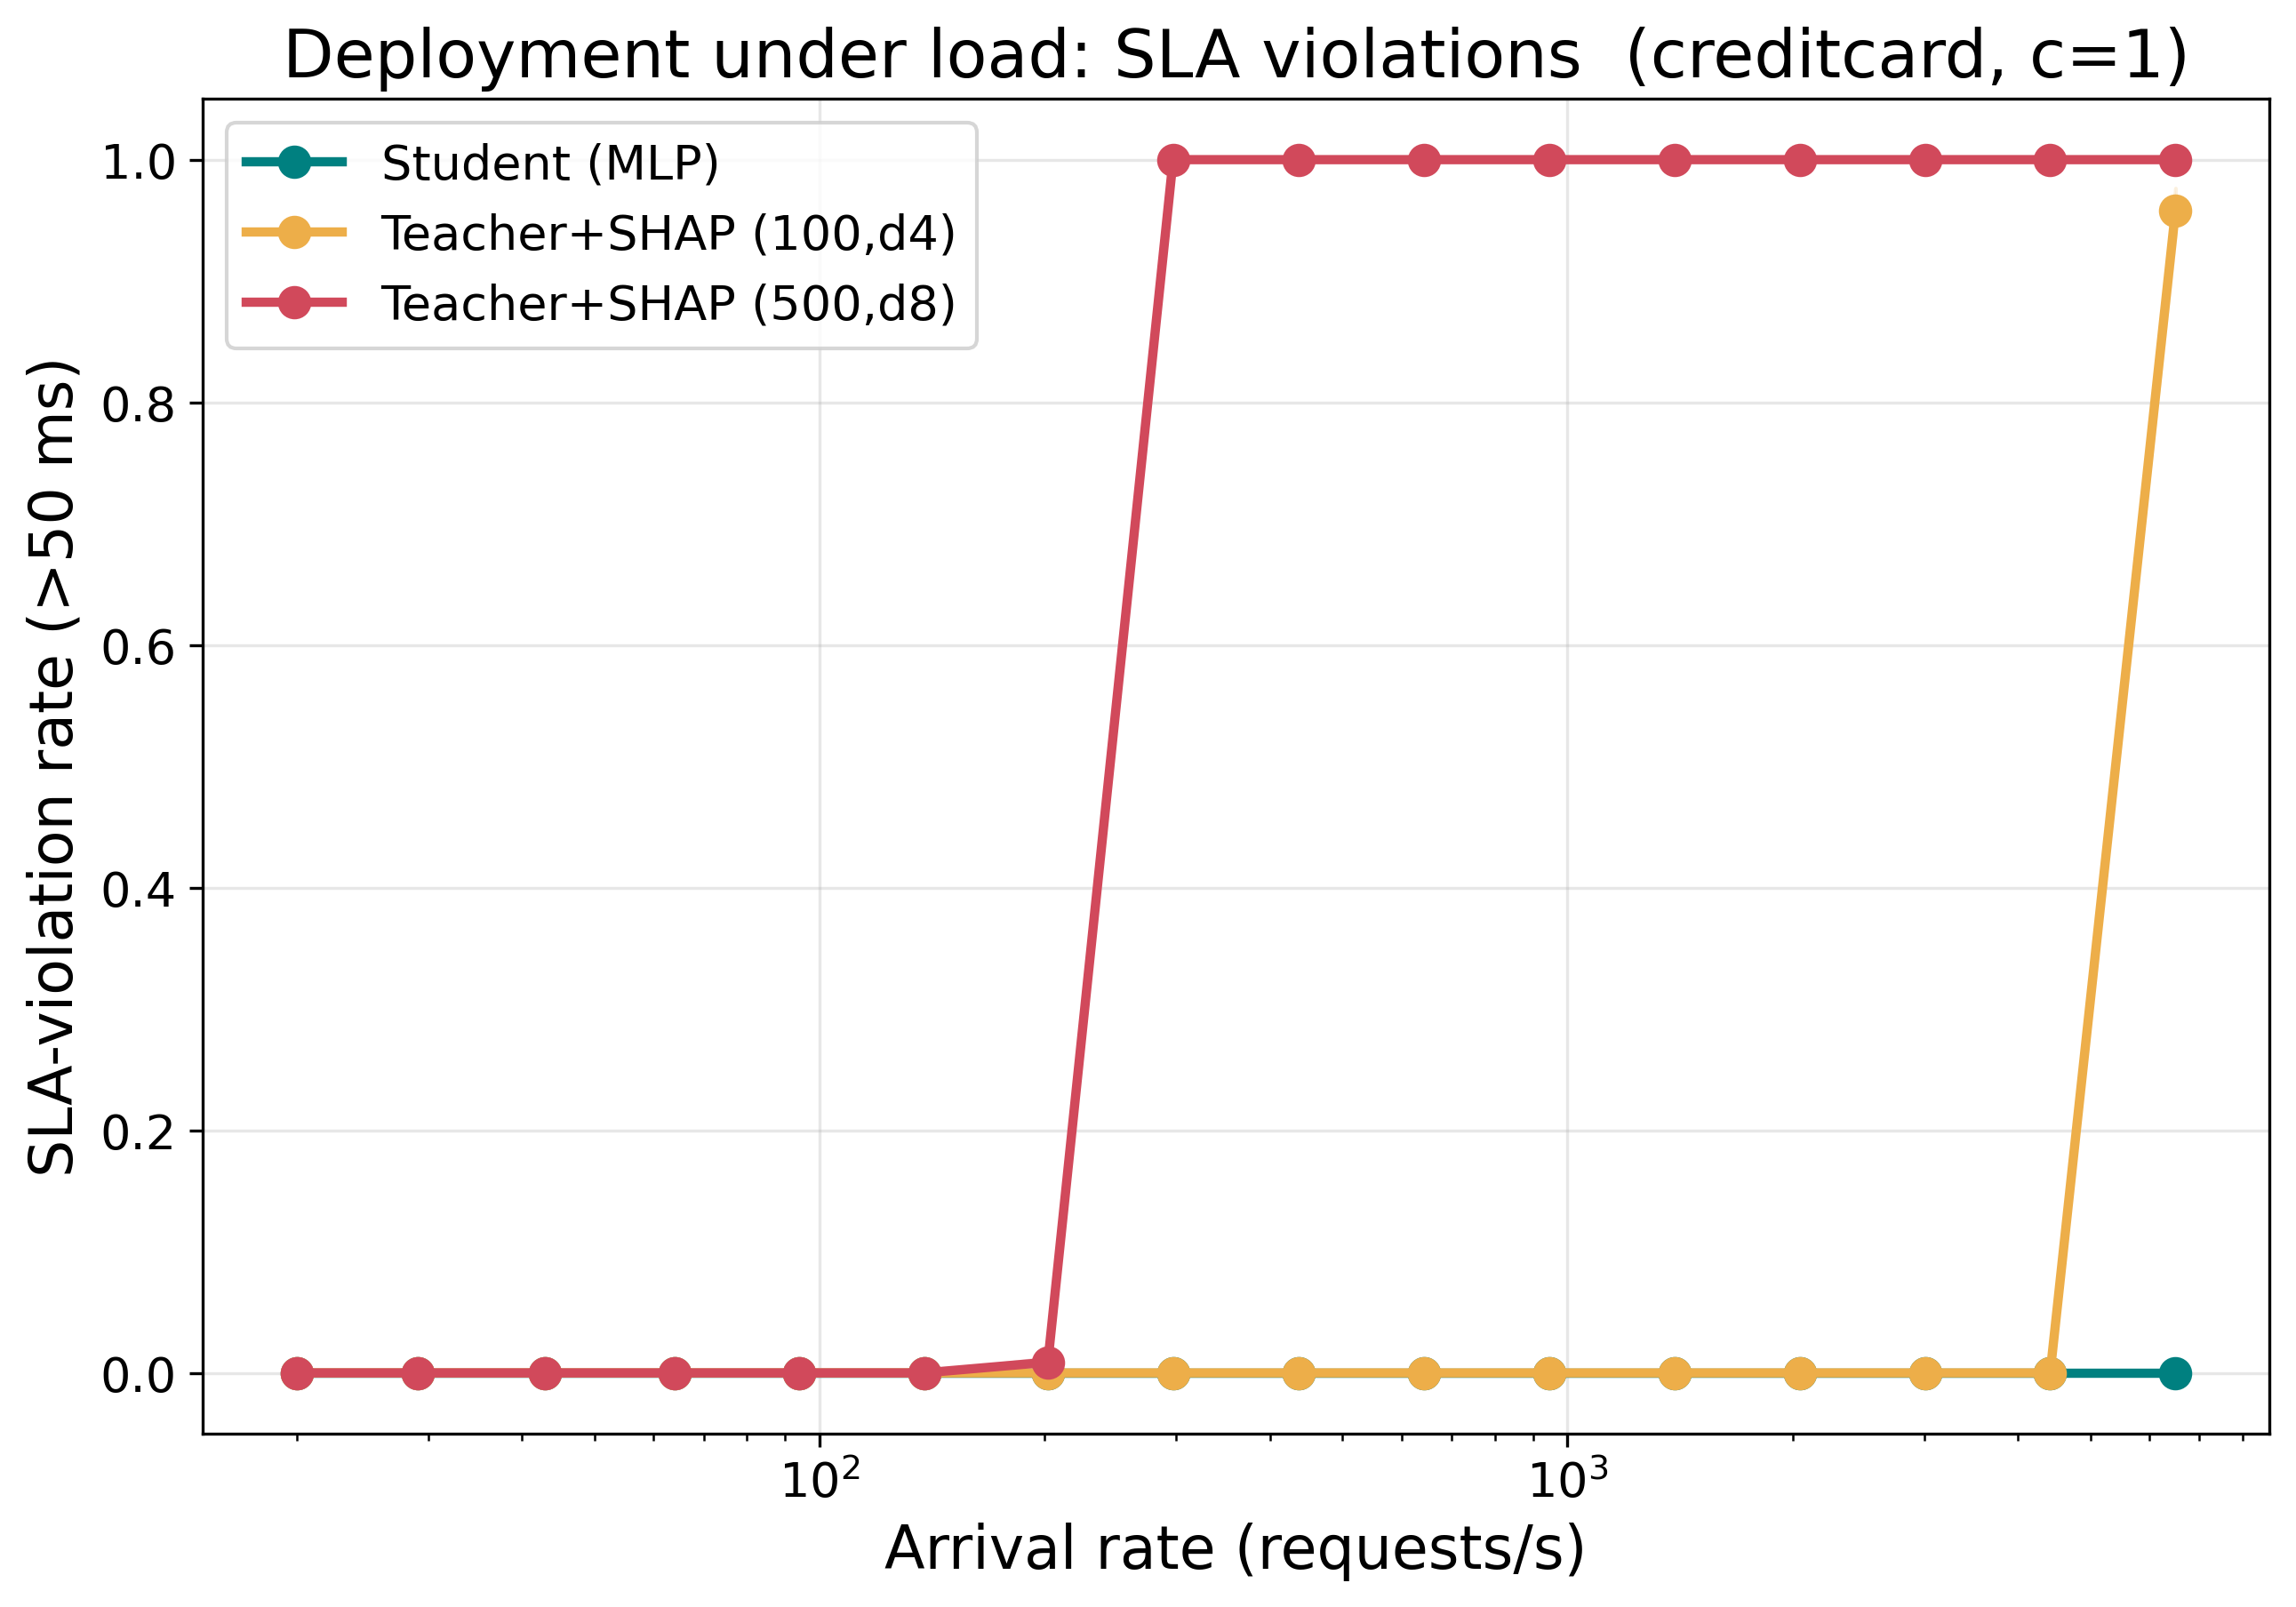
\includegraphics[width=0.46\columnwidth]{fig_wsc_eloi/fig_des_sla.png}\hfill
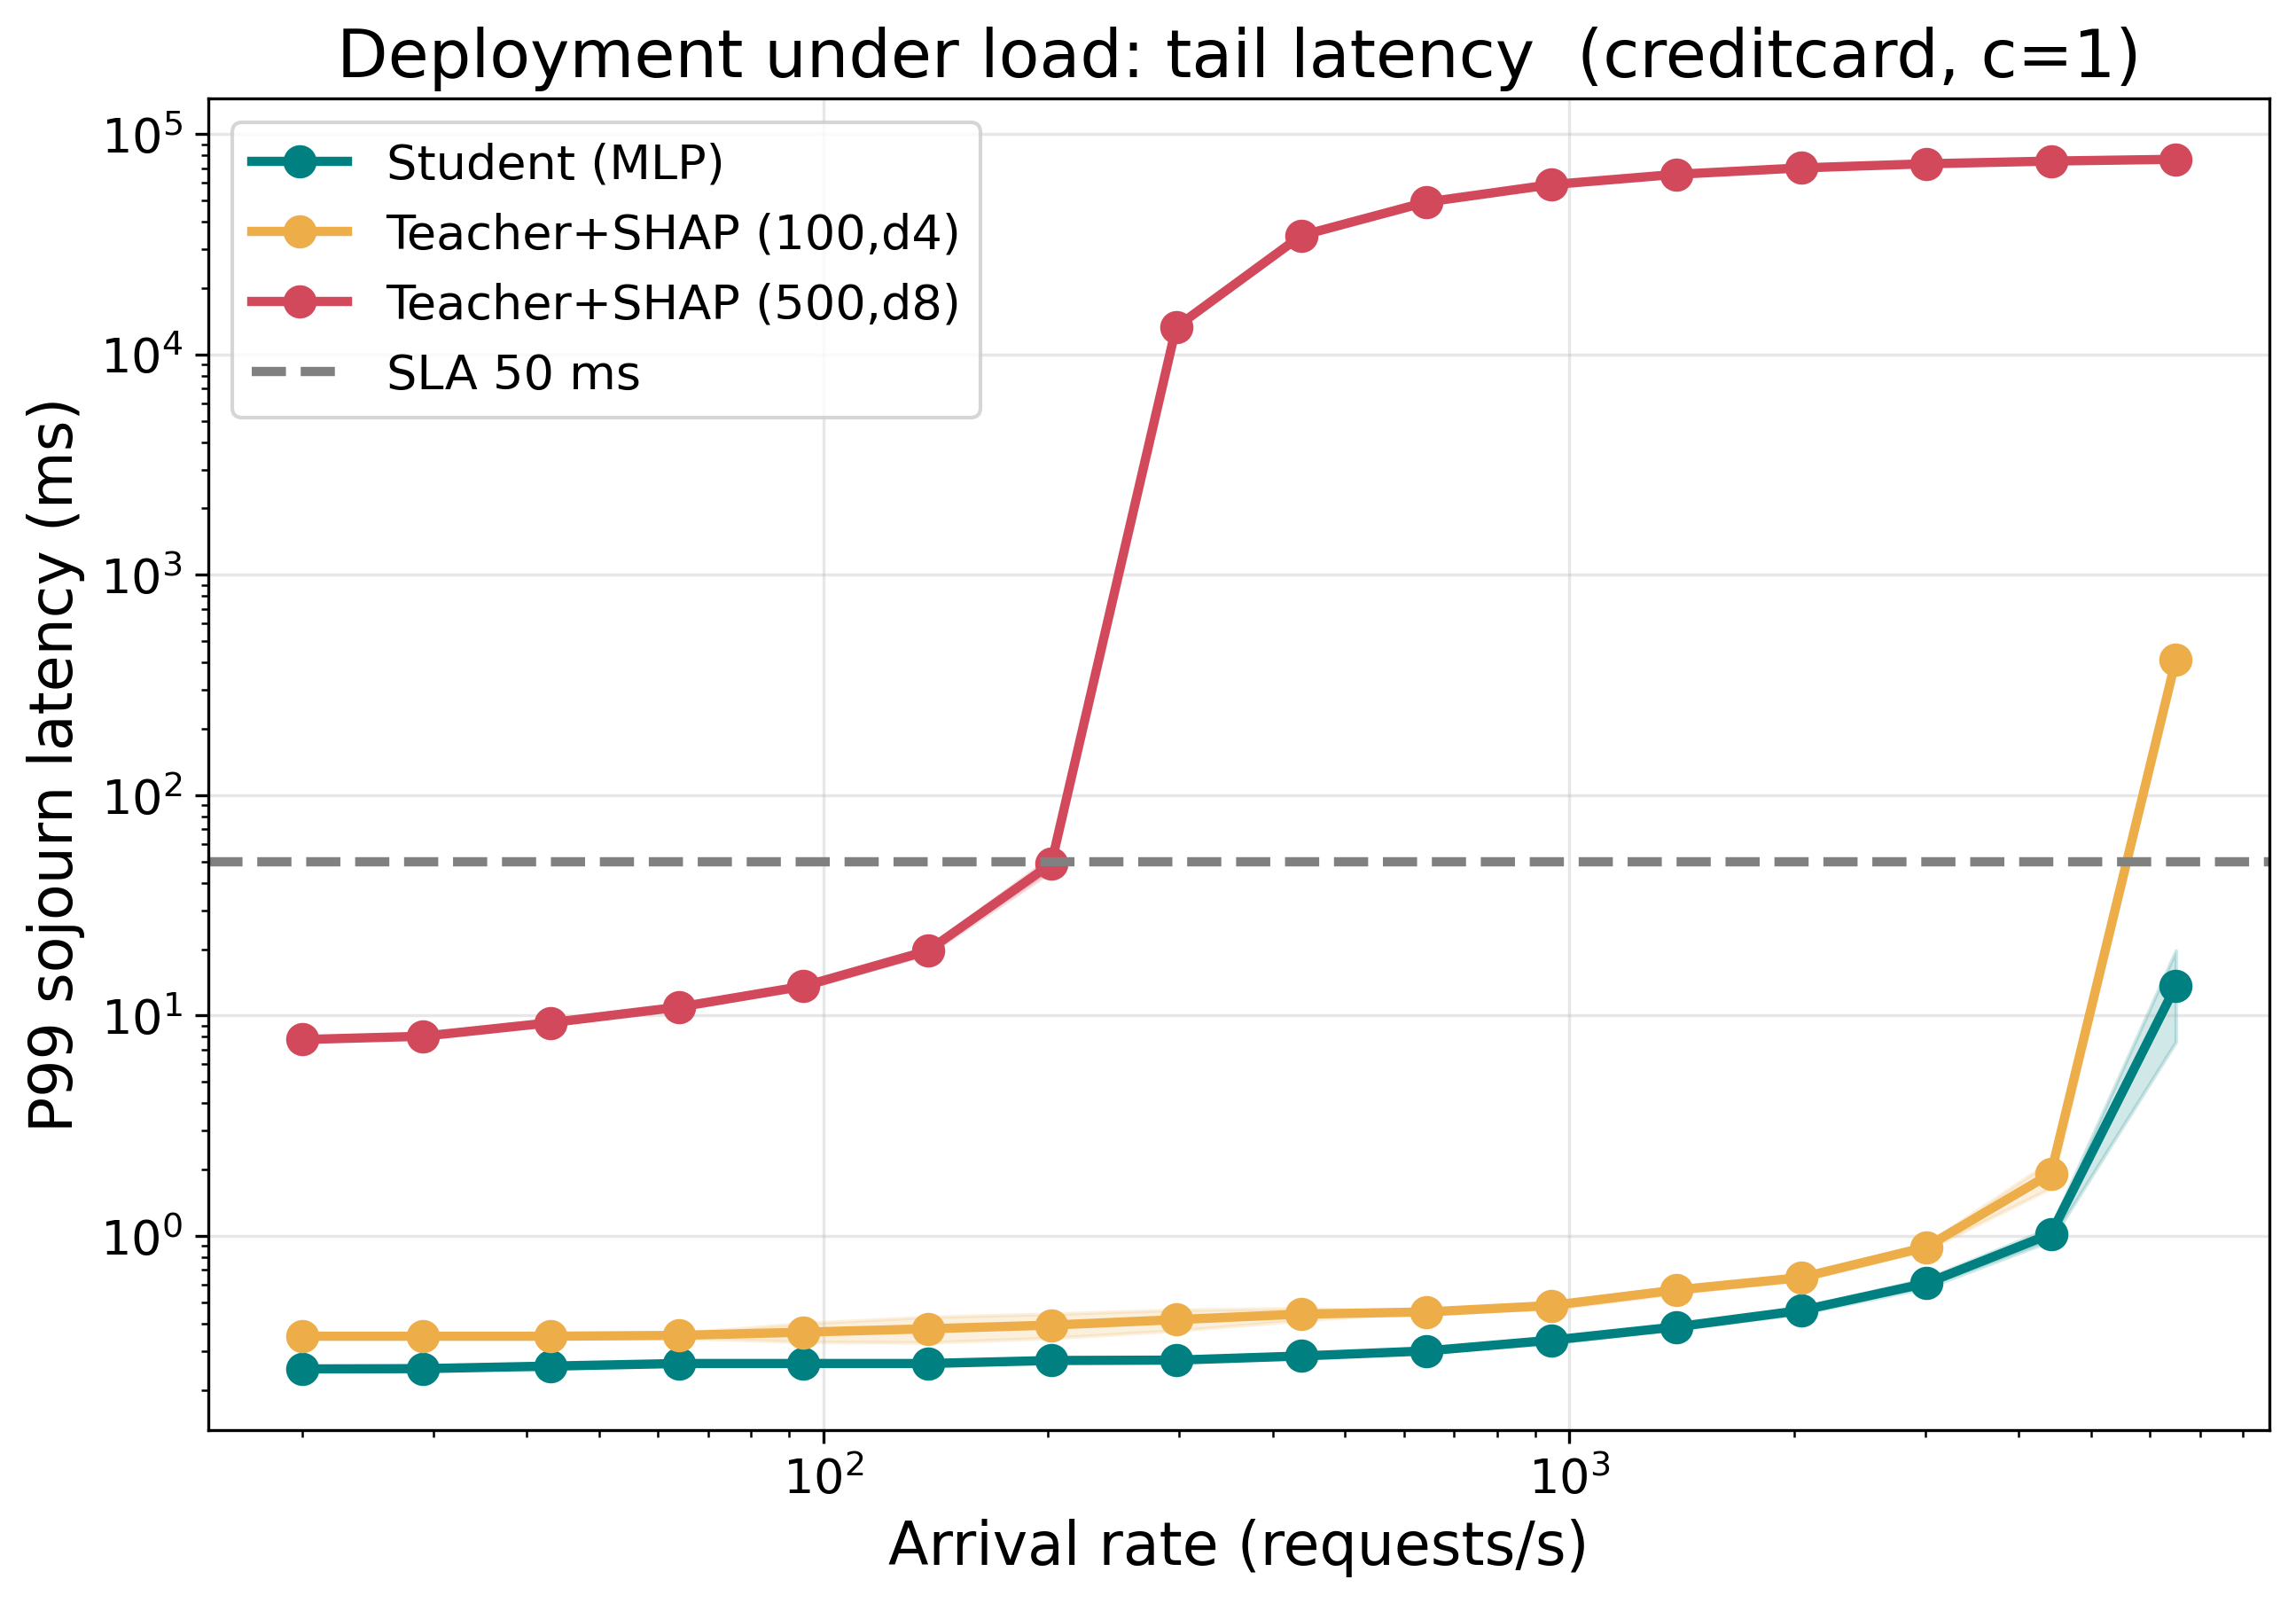
\includegraphics[width=0.46\columnwidth]{fig_wsc_eloi/fig_des_p99.png}
\caption{Deployment simulation (UCI Credit Card service times, single server, 50 ms SLA): SLA-violation rate (left) and P99 sojourn latency (right) vs.\ Poisson arrival rate, with 95\% CI bands. The accurate Teacher+TreeSHAP route saturates near 250 req/s; the Student serves thousands of req/s within SLA.}
\label{fig:des}
\end{figure}

\section{DISCUSSION}
\label{sec:discussion}

The replicated experiment across three datasets clarifies how the Teacher--Student framework addresses the accuracy-explainability-fairness trilemma. On the serving side, the Student delivers risk score and explanation in one forward pass with sub-millisecond P99 latency and one-to-three million samples/s batched throughput, and the discrete-event simulation shows it sustains $\sim$27$\times$ the load of an accurate Teacher+TreeSHAP path before breaching a 50 ms SLA \cite{Boehm2025ScalableSHAP,jethani2022fastshap,Nvidia2023Triton}. We deliberately temper the headline speedup: against the \emph{submitted} small Teacher the per-request gap is modest ($\approx1.2\times$); the order-of-magnitude and throughput advantages appear for accurate ensembles and, decisively, under concurrent load.

The central fairness finding is that the demographic-parity penalty's behavior is governed by protected-group prevalence rather than by sample size alone. When the protected group is well represented (UCI Credit Card, $46.9\%$) the penalty removes bias at no statistically significant accuracy cost; when it is small (Bank Marketing, $2.7\%$) it produces a genuine ``cost of fairness'' (AUC $0.926\!\to\!0.897$) and, notably, \emph{worsens} the Equal-Opportunity gap even as it improves demographic parity \cite{Hardt2016Equality}; when it is tiny (German Credit, 31 instances) the in-batch estimate is so noisy that the penalty becomes unreliable. We therefore retract the earlier suggestion that fairness regularization improves accuracy on institution-scale data: under multi-seed replication those gains are within noise, and on Bank Marketing the trend reverses. The stabilized L1 penalty and homoscedastic balancing \cite{DBLP:journals/corr/KendallGC17} remain valuable for keeping optimization stable---no run diverged---but their fairness benefit is conditional on adequate group representation, a nuance the simulation study makes explicit and actionable for practitioners.

\section{CONCLUSION}
\label{sec:conclusion}

This paper has demonstrated, through a replicated simulation study, a methodology for deploying responsible AI in high-frequency financial environments. By distilling complex tree ensembles into a label-supervised multi-task network, we serve risk scores and intrinsic explanations in a single forward pass with sub-millisecond latency, and a discrete-event simulation quantifies the resulting throughput headroom under load \cite{jethani2022fastshap,Boehm2025ScalableSHAP}. The scenario-based experiment characterizes the teacher--student interaction with proper replication and confidence intervals, and yields an honest, actionable picture of the trilemma: the stabilized demographic-parity penalty mitigates bias at no significant accuracy cost when the protected group is well represented, but incurs an accuracy trade-off---and can conflict with equal opportunity---when the group is scarce \cite{Hardt2016Equality}. The architecture supports the explanation and fairness requirements of the EU AI Act and GDPR by design \cite{Chee2024EULaw,Hunton2023CJEU}. Future work will fold the fairness term into the homoscedastic balancing, extend the equal-opportunity penalty and the deployment simulation (multi-server scaling, batching policies), and generalize to non-binary sensitive attributes and other high-stakes domains.



% \subsection{Citing a Reference}
% To cite a reference in the text, use the author-date method. Thus, \citeN{chi89} could also be cited parenthetically \cite{chi89}.
% Do not use a comma within this parenthesis.
% For a work by three or more authors, use an abbreviated form. For example, a work by Banks, Carson, and Nelson would be cited in one of the following ways: \shortciteN{bcnn:simulation} or \shortcite{bcnn:simulation}.

% Parenthetical citations are enclosed in parentheses $(~)$, not square brackets $[~]$.
% Semicolons separate the items in a series of such citations.

% The following is a list of correct forms of citations:
% \begin{itemize}
% \item Brown and Edwards (1993)
% \item (Brown and Edwards 1993)
% \item (Smith 1987; Brown and Edwards 1992; Brown et al. 1995)
% \end{itemize}

% The following is a list of \textbf{incorrect} forms of citations:
% \begin{itemize}
% \item Brown and Edwards [1993]
% \item (Brown and Edwards, 1993)
% \item (Smith, 1987; Brown and Edwards, 1993)
% \item (Smith 1987, Arnold, Brown and Edwards 1992, Brown et al. 1995)
% \end{itemize}


% \section{GENERAL GUIDELINES}

% \subsection{Language}
% The paper should be prepared using U.S. English in the interest of consistency across the proceedings. Please carefully check the spelling of words before you submit your paper. There are spell checkers for \LaTeX\ as well.
% Some examples of software which supports spell checking are TexnicCenter, TexMaker, and TexClipse.

% \subsection{Paper Submission}
% You will submit the Portable Document Format ({\tt .pdf}) of your paper electronically at the \href{http://www.wintersim.org}{conference website}. Source files (text, graphics, bib) are not needed. If the paper is accepted, you will electronically submit the \LaTeX source file ({\tt .tex}) for the final version of your paper in a ZIP format that includes all figures and auxiliary files.
% The editors may send the file back to you with the request to make changes to conform to conference guidelines. For minor changes, the editors may make the changes themselves. Final {\tt .pdf} files are generated by the conference proceedings editors.

% You will also need to transfer the copyright of your article to the WSC using the copyright transfer form that will be available via the conference web site at the appropriate time. {\em For your paper to be published by the WSC, you must complete the transfer of copyright.}
% When you have successfully transferred the copyright, you will receive a {\tt .pdf} receipt.

% If you are unable to satisfy these requirements, you should contact the proceedings editors.

% \subsection{Objectivity}
% The content of the paper should be objective and without any appearance of commercialism. In general, comparisons of commercial software should be avoided unless they are central to the topic. If a comparison of commercial software is included, it should be based on objective analysis that includes criteria, description of ranking methodology on each criterion, and the rankings themselves to arrive at a conclusion. If an approach other than a detailed objective analysis is used to select the simulation software used for the study being reported, such as, availability of the software, or the familiarity of the analyst with the software, it should be clearly identified.

% \subsection{Length Constraints}

% \subsubsection{Length of the Abstract}
% The abstract should be at most 150 words. Since abstracts of all papers accepted for publication in the proceedings will also appear in the final program, the length limit of 150 words will be strictly enforced for each abstract. The abstract should consist of a single paragraph, and it should not contain references or mathematical symbols. Do not include a list of keywords. Keywords are not used in WSC proceedings.

% \subsubsection{Length of the Paper}
% The page size in the proceedings must be 8.5 inches by 11 inches (21.6 cm by 27.9 cm). The overall length of the paper should be at least 5 proceedings pages. \textbf{Papers should be at most twelve (12) pages,} except for introductory tutorials, advanced tutorials, and panel sessions, for which the limit is 15 pages. Exceeding the page limit will result in rejection for the proceedings.

% \subsection{Font Specification and Spacing}
% The paper should be set in the Times New Roman font using a 11-point font size. The paper should be single spaced. Do not use other fonts; use of other fonts means the proceedings editors will need to send the paper back to you to change the font.

% \subsection{Margins}
% \label{sec:margins}
% The width of the text area is 6.5 inches (16.5 cm). The left and right margins should be 1 inch (2.54 cm) on each page. Except for the first page, the top and bottom margins should be 1 inch (2.54 cm). First page has 1.5 inch (3.81 cm) margin from the title to the top of the page, and 1 inch bottom margin. Authors should neither change the header and footer settings nor the corresponding \LaTeX\ style when preparing a manuscript.

% \subsection{Justification}
% Headings of sections, subsections, and subsubsections should be left-justified. One-line captions for figures or tables should be centered. A multiline caption for a figure or table should be fully justified. All other text should be fully justified across the page (that is, the text should line up on the right-hand and left-hand sides of the page).

% \subsection{Headings of Sections, Subsections, and Subsubsections}
% Section, subsection, and subsubsection headings should appear flush left, set in the bold font style, and numbered as shown in this document. The headings for the Abstract, Acknowledgments, References and Author Biographies sections are not numbered. Section headings should be set in \textbf{FULL CAPITALS LIKE THIS PHRASE}, while subsection and subsubsection headings should be \textbf{Capitalized in Headline Style like This Phrase}. Lengthy headings should be broken across two or more lines. \textbf{Again, these formats should be accomplished using section, subsection, subsubsection, etc.}

% \subsubsection{Paragraphs}
% The first paragraph after a heading should not be indented; all other paragraphs should be indented by 0.25 inches (0.63 cm). Do not insert additional space between paragraphs.

% Programming code should use ``Program Start'', ``Program'', and ``Program End'' Styles with the following guidelines.

% \begin{verbatim}
% class Exponential{
% ...// Properties of the Exponential
% };
% \end{verbatim}

% One-line programs should use the ``Program Both'' style.

% \begin{verbatim}
% Exponential interArrival;
% \end{verbatim}

% \subsubsection{Footnotes}
% \textbf{Do not use footnotes}; instead incorporate such material into the text directly or parenthetically.

% \subsubsection{Page Numbers}
% Do not include page numbers. Page numbers are generated by the proceedings editors once all accepted papers are ordered for the final proceedings.

% \section{FORMATTING THE FIRST PAGE}

% \subsection{Running Heads}
% The running head (provided in the template) in the upper left-hand corner of the first page (which should read {\em \currentCaption}\dots) is left-justified and set in the 11-point italic font style. You do not have to change the content of the first-page header; the first-page header was set by the proceedings editors in the preparation of this document.

% Running heads on the second and subsequent pages should contain the last names of the authors, centered and set in the 11-point italic font style. For example, running heads for papers would appear like \textit{Justme} for papers with one author, or \textit{Justme and Him} for papers with two authors, or \textit{Justme, Him, and Youtoo} for papers with three authors, etc. These are created by using the macro\newline

% \begin{verbatim}
% \WSCpagesetup{LastName1, LastName2, and LastNameLastAuthor}

% \end{verbatim}
% defined in the class file.
% Please use this macro to set up the running heads, as it sets further parameters important for the correct layout of the document.

% The author names are listed in the same order as they appear on the title page, which is the same order the author biographies are provided.
% These entries {\bf do} need to be changed by the authors in the {\tt $\backslash$WSCpagesetup} command in the source for this file.
% Please give all author names and do not use \textit{et al.}, except in the rare situation where they don't fit on one line. In the latter case, only the first author is given followed by ``et al.''.


% \subsection{Title and Authors}
% Center the title of the paper across the page and set it in bold {\bf FULL CAPITALS} so that the top edge of the title begins 1.5 inches from the top of the page.
% The correct placement is automatically done by the class file as well.
% Just use the {\tt $\backslash$title} and {\tt $\backslash$maketitle} commands as it is done in the source of this document.
% Multiline titles should have about the same amount of text on each line.

% There should be 2 blank lines between the title and the authors' names (will be inserted by the class file if the {\tt $\backslash$author}, {\tt $\backslash$title}, and {\tt $\backslash$maketitle} commands are used).

% All authors' names should have initial letters capitalized, and be listed on a line in a centered fashion, with the author's first name first and no job title or honorific. In the case of many authors, multiple centered lines might be used to list all authors. Behind each author's name is superscript \textsuperscript{1}, \textsuperscript{2}, \textsuperscript{3}, etc. denoting the author's affiliation. If an author has multiple affiliations, then only the main affiliation should be listed unless it is strictly necessary to use multiple affiliations, in which case the superscript could consist of multiple indices, e.g., \textsuperscript{1,2}. On the other hand, each affiliation could apply to multiple co-authors.
% These affiliations are detailed under the authors' names, with one blank line between authors' names and the affiliation details. Each affiliation starts with the superscript index, then the department, institution, city, standard two-letter state or province abbreviation, and country. The state abbreviation and country name should be in FULL CAPITALS.
% Each affiliation should be detailed in a single centered line to the extent possible, by using common abbreviations, e.g., ``Dept.'' for ``Department'', ``Eng.'' for ``Engineering'' and other common-sense abbreviations if needed. However, using multiple lines is acceptable if a single line is not sufficient to detail the affiliation even after a reasonable effort to abbreviate.
% For papers with multiple authors, the authors should be listed in order of decreasing contribution. Some examples of title page heading and common-sense abbreviations are shown in Figures~\ref{fig:different}--\ref{fig:two lines} and Table~\ref{table:abbreviation} respectively at the end of this document. There should be two blank lines between the author fields and the text of the paper. Do not include email addresses on the first page; emails for authors are provided in the author biographies.


% You should use the {\tt $\backslash$author} command to enter author names -- see the source for this document.

% \section{FORMATTING SUBSEQUENT PAGES}
% Please refer to Section~\ref{sec:margins} for the correct margins.

% \subsection{Mathematical Expressions in Text and in Displays}
% Display only the most important equations, and number only the displayed equations that are explicitly referenced in the text.
% To conserve space, simple mathematical expressions such as $\bar Y = n^{-1} \sum_{i=1}^n Y_i$ may be incorporated into the text.
% Mathematical expressions that are more complicated or that must be referenced later should be displayed, as in
% $$s^2 = \frac 1 {n-1} \sum_{i=1}^n (Y_i - \bar Y)^2.$$

% If a display is referenced in the text, then enclose the equation number in parentheses and place it flush with the right-hand margin of the
% column. For example, the quadratic equation has the general form

% \begin{equation} \label{eq:quadratic}
% ax^2 + bx + c = 0, \mbox{ where } a \ne 0.
% \end{equation}

% In the text, each reference to an equation number should also be enclosed in parentheses. For example, the solution to (\ref{eq:quadratic}) is given in (\ref{eq: quadratic sol}) in Appendix \ref{app:quadratic}.

% If the equation is at the end of a sentence, then you should end the equation with a period. If the sentence in question continues beyond the equation, then you should end the equation with the appropriate punctuation -- that is, a comma, semicolon, or no punctuation mark. If the equation is not included within any sentence, but just given between two paragraphs, no punctuation is used as in equation (\ref{eq:quadratic_second}).

% \begin{equation} \label{eq:quadratic_second}
% ax^2 + bx + c = 0
% \end{equation}

% \subsection{Displayed Lists}
% A displayed list is a list that is set off from the text, as opposed to a run-in list that is incorporated into the text. The bulleted list given below provides more information about the format of a displayed list.

% \begin{itemize}
% 	\item Use standard bullets instead of checks, arrows, etc.\ for bulleted lists.
% \end{itemize}
% \begin{enumerate}
% 	\item For numbered lists, the labels should not be arabic numerals enclosed in parentheses because such labels cannot be distinguished from equation numbers.
% \end{enumerate}

% Indent the paragraph after the list.

% \subsection{Figures and Tables}
% \label{sec:graphics}
% Figures and tables should be centered within the text and should not extend beyond the right and left margins of the paper.
% Figures and tables can make use of color since the WSC produces electronic proceedings.
% However, try to select colors that can be differentiated when printing in black and white in consideration of people using such printers. Figures and tables are numbered sequentially, but separately, using arabic numerals.
% All tables and figures should be explicitly referenced in the text and they should not be placed before they are referenced.
% The reference is always written in full (Figure 1), and never abbreviated as in ``(Fig. 1)''.
% For figures which can fit next to each other, the author can choose to align them next to each other with the figure text centered below each figure and on the same line for both figures. For tables which can fit next to each other, the author can also choose to align them next to each other with the table text centered above each table and on the same line for both tables.

% The table's one-line captions are centered, while multi-line captions are fully justified.
% The captions appear {\em above} the table.
% Captions can be written using normal sentences with full punctuation. All captions should end with a period. It is fine to have multiple-sentence captions that help to explain the table.
% See Tables \ref{tab: first} and \ref{tab: second} for examples.

% \begin{table}[htb]
% \centering
% \caption{Table captions appear above the table, and if they are longer than one line they are fully justified. Captions are written using normal sentences with full punctuation. It is fine to have multiple-sentence captions that help to explain the table.\label{tab: first}}
% \begin{tabular}{rll}
% \hline
% Creature & IQ & Diet\\ \hline
% dog & 70 & anything\\
% human & 60 & ice cream \\
% dolphin & 120 & fish fillet\\
% \hline
% \end{tabular}
% \end{table}

% \begin{table}[htb]
% \centering
% \caption{Comparison between samples.\label{tab: second}}
% \begin{tabular}{|r|l|}
% \hline
% Sample & Height (cm) \\ \hline
% Plant one & 50 \\ \hline
% Plant two & 58 \\
% \hline
% \end{tabular}
% \end{table}

% Captions end with a period. One-line captions are centered, while multiline captions are fully justified. Figure captions appear below the figure. See Figures \ref{fig: tahi} and \ref{fig: rua} for examples.

% \begin{figure}[htb]
% {
% \centering
% %\includegraphics[width=0.9\columnwidth]{MathExpandExpression.jpg}
% \includegraphics[width=0.50\textwidth]{MathExpandExpression}
% \caption{An unusual answer to a question.\label{fig: tahi}}
% }
% \end{figure}

% \begin{figure}[htb]
% {
% \centering
% %\includegraphics[width=0.9\columnwidth]{puzzle.png}
% \includegraphics[width=0.50\textwidth]{puzzle}
% \caption{The area of the square is 64 squares, while that of the rectangle is 65 squares, yet they are made of the same pieces! How
% is this possible? \label{fig: rua}}
% }
% \end{figure}

% References to tables and figures identified by number are capitalized. Avoid using ``in the previous table'' or ``in the figure below'', as positions might change in the final formatting. Be sure to use the {\tt $\backslash$label} command within the figure or table environment and refer to the associated figure or table using {\tt Table$\sim \backslash$ref\{labelgiven\}}.
% Please do not use hard coded figure/table numbers. This is error prone, and the references will not be hyperlinks.

% Please ensure that the text within figures uses standard fonts and is readable: Arial (recommended), Symbol, etc. The minimum font size should be around 9pt (Arial). Remember that you might need larger fonts in your original figure if you reduce the size of the figure in your WSC paper to less that 100\% (e.g., when you insert your figure with a 50\% of its original size, your original fonts have to be $>=$18pt). This applies to all text elements in the figure, including captions of axes, etc.

% Including graphics files in your document can be complicated.
% Use {\tt .jpg}, {\tt .png} or {\tt .pdf} files.
% The main difference between the formats is how they store the images and how well suited they are for specific graphics. You can choose between bitmap and vector graphics.
% Bitmap graphics are well suited for photographs (jpg is very common here) or for screenshots (PNG is a lossless encoding in contrast to jpg, and is thus better suited for all those cases where you have sharp edges in your graphics).
% Vector graphics are the encoding to be chosen for all kinds of drawings (diagrams, charts, ...). In contrast to bitmap formats, they can be scaled to any size without any loss of sharpness. This makes it possible to read such graphics even if two pages are printed on one sheet of paper, or if the documents are read electronically.
% So what to choose for your \LaTeX\ document? As a rule of thumb you should always prefer PDF or PS and EPS.
% In general these three encodings can contain both, bitmap and vector graphics. But there is no need (and no use) to convert your bitmaps to any of these.

% Use the {\tt PDFLaTeX} command to generate your pdf file, as was done with this file.
% The final file format is PDF.
% If you include figures via {\tt includegraphics}, then please do so without the file ending (e.g., skip .pdf, .ps, ...).

% \subsection{Definitions and Theorems}
% Definitions, theorems, propositions, etc. should be formatted like a normal paragraph with boldface heading as shown in the examples below. Number
% these items separately and sequentially. You may choose not to separately number theorems, propositions, corollaries, etc., as opposed to the example below where corollaries and theorems are numbered together. Search the source of this document to see how these environments were defined. The key
% command is {\tt $\backslash$newtheorem}. Do not use a period after the definition, theorem, corollary or proposition \textit{number}, but do end the sentence with a period.

% \begin{definition}
% In colloquial New Zealand English, the term {\em dopey mongrel} is used to refer to someone who has exhibited less than stellar intelligence.
% \end{definition}

% \begin{theorem}
% If a proceedings editor from New Zealand accidentally deletes his draft of the author kit shortly after completing it, he would be considered to be a dopey mongrel.
% \end{theorem}

% \begin{corollary}
% One of the proceedings editors is a dopey mongrel.
% \end{corollary}

% Indent the paragraph after the definition or theorem.

% \subsection{Hyperlinks}
% \label{sec: hyper}
% A {\em hyperlink} specifies a web address (URL) or an email address.
% The use of hyperlinks allows authors for providing readers access to external electronic information, such as a dynamic simulation or animation.
% The use of hyperlinks is at the discretion of the author(s).
% {\bf While the use of hyperlinked text is encouraged in the main body of the paper, it is recommended that corresponding web addresses and other identifying information should be provided in the list of references.}
% For example, instead of spelling out the web address of the conference website, one would refer to the \href{http://www.wintersim.org}{conference website}~\cite{WSC}, and the corresponding entry in the reference section will spell out the associated web address and other relevant information such as author(s) and/or the organization that published the content.
% This would allow readers for searching for the content using the author(s), organization, etc. if the actual web address is changed. This also allows for a cleaner appearance of the main body of the paper.

% If the author(s) feel that sufficient information is provided in the main body of the paper to locate the content even if the web address is changed, the address can be included in the main body of the paper itself.

% Each hyperlink should be set in the same font as the text.
% Hyperlinks are {\em not} underlined.
% A live hyperlink (or hot link) -- that is, a hyperlink that will activate your web browser and take it to an external web site or that will activate your email software for sending a message to a specific email address -- should be colored blue. You have already seen examples of such hyperlinks in this paper.
% To use live hyperlinks in a proceedings paper, use the {\tt hyperref} package. If you are using {\tt PDFLaTeX} to generate your pdf file then, as
% was done for this file, you should add the following as the last {\tt $\backslash$usepackage} command in the preamble.\newline


% \begin{verbatim}
% \usepackage[pdftex,colorlinks=true,urlcolor=blue,citecolor=black,
% anchorcolor=black,linkcolor=black]{hyperref}
% \end{verbatim}\vspace{5 mm}

% \noindent On the other hand, if you are using the traditional {\tt latex - dvips - ps2pdf} route, then users of MiKTeX or PCTeX for Windows should add the command\newline


% \begin{verbatim}
% \usepackage[dvips,colorlinks=true,urlcolor=blue,citecolor=black,
% anchorcolor=black,linkcolor=black]{hyperref}
% \end{verbatim}\vspace{5 mm}


% \noindent as the last {\tt $\backslash$usepackage} command in the preamble, while users of Y\&Y TeX should add the command\newline


% \begin{verbatim}
% \usepackage[dvipsone,colorlinks=true,urlcolor=blue,citecolor=black,
% anchorcolor=black,linkcolor=black]{hyperref}
% \end{verbatim}\vspace{5 mm}


% \noindent as the last {\tt $\backslash$usepackage} command in the preamble.
% (In general the {\tt $\backslash$usepackage} command above that works for MiKTeX running on a Windows system should also work for most implementations of \LaTeX\ running on a Unix or Apple system.)
% Thus the hypertext link \href{http://www.wintersim.org}{conference website}~\cite{WSC} to the WSC website can be established by the command\newline

% \begin{verbatim}
% \href{http://www.wintersim.org}{conference website}
% \end{verbatim}\vspace{5 mm}


% \noindent This is especially important since WSC papers are filed in the IEEE Xplore digital library, which does not allow hyperlinks, so for that purpose the hyperlinks are removed.
% Therefore it is recommended to add all hypertext references to the {\tt .bib} file and to refer to them from the text as it is done in the example above.
% All live hyperlinks still appear in the CD of the proceedings and in other repositories.

% If you use the package {\tt hyperref} as suggested here, and if you use citation commands to handle references, then your citations will
% become hyperlinks (as in this document).

% Non-live hyperlinks -- that is, the hyperlinks that are included for the reader's information but do not actually invoke the reader's web browser or email software should be colored black.

% \subsection{Citing a Reference}
% To cite a reference in the text, use the author-date method. Thus, \citeN{chi89} could also be cited parenthetically \cite{chi89}.
% Do not use a comma within this parenthesis.
% For a work by three or more authors, use an abbreviated form. For example, a work by Banks, Carson, and Nelson would be cited in one of the following ways: \shortciteN{bcnn:simulation} or \shortcite{bcnn:simulation}.

% Parenthetical citations are enclosed in parentheses $(~)$, not square brackets $[~]$.
% Semicolons separate the items in a series of such citations.

% The following is a list of correct forms of citations:
% \begin{itemize}
% \item Brown and Edwards (1993)
% \item (Brown and Edwards 1993)
% \item (Smith 1987; Brown and Edwards 1992; Brown et al. 1995)
% \end{itemize}

% The following is a list of \textbf{incorrect} forms of citations:
% \begin{itemize}
% \item Brown and Edwards [1993]
% \item (Brown and Edwards, 1993)
% \item (Smith, 1987; Brown and Edwards, 1993)
% \item (Smith 1987, Arnold, Brown and Edwards 1992, Brown et al. 1995)
% \end{itemize}

% \subsection{General Style and Sequence of References}
% Place the list of references after the appendices. The section heading is {\bf REFERENCES}, and it is not numbered. List only references that are cited in the text. Do not number the references. The only exception are papers in the ``tutorial'' tracks: Here it is permitted to have an additional section heading {\bf ADDITIONAL READING} after references, followed by further literature that is recommended for continued studies but not directly used within the text of the paper

% Do not number the references and arrange them in the following order:
% \begin{itemize}
% 	\item By the last name of the first author.
% 	\item For papers with the same first author, arrange first all papers by this author only, then all papers by this author and one co-author, and finally all papers with this author and two or more co-authors.
% \item Within this sorting sequence, arrange papers by year.
% \end{itemize}

% To identify multiple references by the same authors and year, append a lower case letter to the year of publication; for example, 1984a and 1984b. The same applies to references that have more than two authors and the same first author and year.

% Give complete references without abbreviations. List \underline{all} authors except when there are more than six authors, in which case the first six author names are shown followed by ``\textit{et al.}''.
% %Only if you cite a book contribution with the book having more than two editors, abbreviate to the first editor ``et al.''.

% The format for other types of reference as well as examples can be inferred from the examples in the references section, which include:
% \begin{itemize}
% \item A technical report \cite{chi89}
% \item A proceedings article \cite{cheng:input94}
% \item A conference contribution without book publication \shortcite{rabe:combining}
% \item A journal article with two authors \cite{powell2017widening}
% \item A journal article with more than two authors \shortcite{gupta:mnormal}
% \item A book by two authors \cite{hammersley:montecarlo}
% \item A chapter in a book \cite{sch79}
% \item An unpublished thesis or dissertation \cite{ste99}
% \item A book with no identified authors \cite{chicago03}
% \item A document available on the web \cite{WSC}
% \end{itemize}

% Be sure that references to past WSC proceedings include the necessary information, as in \citeN{cheng:input94} and \citeN{hunter:clm22}. This information and the template can be exported as bibtex code by the IEEE website for the considered paper. Below is a template for a bib entry of a (yyyy) Winter Simulation Conference proceedings paper:

% \begin{verbatim}

% @INPROCEEDINGS{(!!Provide a unique key here!!),
% 	author={aaaa},
% 	title={tttt},
% 	year={yyyy},
% 	volume={}, % you can leave empty
% 	number={}, % you can leave empty
% 	pages={n-m},
% 	booktitle={yyyy Winter Simulation Conference (WSC)},
% 	doi={10.1109/WSC.....}
% }

% \end{verbatim}

% Please do not add any additional attributes.


% \subsection{Formatting References According to Their Type of Publication}

% Use hanging indentation to distinguish individual entries. Do not insert additional space between references.

% You can enter the references using (a) {\em \BibTeX\ as discussed in Section~\ref{sec:bibtex}}, (b) using the environment {\tt thebibliography} via the {\tt $\backslash$bibitem} and {\tt $\backslash$cite} commands, or (c) the {\tt hangref} environment as shown below.
% Please note that neither (b) nor (c) are recommended. These alternatives may mean extra work for you and the editor during the editing process. Option (c) means in addition that the references will not be hyperlinks -- as the proceedings are electronic proceedings this is not recommended at all.

% To use {\tt hangref} you would enter the following lines.

% \begin{verbatim}

% \begin{hangref}
% \item The first reference goes here, and if you happen to have enough
% information on the line you will be able to see how the second and if
% you really have lots of text to be displayed later lines of the
% reference are indented.
% \item The second reference goes here, and once again later lines are
% indented if you have a sufficient amount of words in the text block.
% \item Further references appear here.
% \end{hangref}

% \end{verbatim}

% \subsubsection{Journal Articles}
% The bibliographic style for a journal article is:
% $<$Surname of first author$>$, $<$Author's initial(s)$>$,
% $<$Initials and surnames of other authors$>$. $<$year$>$.
% $<$Capitalized article title in quotes$>$. $<${\em Journal Name in
% Headline Italics}$>$ $<$Volume number$>$($<$issue number$>$):$<$page numbers$>$.

% {\footnotesize
% \begin{hangref}
% \item Gupta, S. S., K. Nagel, and S. Panchapakesan. 1973. ``On the Order Statistics from Equally Correlated Normal Random Variables''. \textit{Biometrika} 60(2):403-413.
% \item Powell, J. H. and N. Mustafee. 2017. ``Widening Requirements Capture with Soft Methods: An Investigation of Hybrid M\&S Studies in Healthcare''. \textit{Journal of the Operational Research Society} 68(10):1211-1222.
% \end{hangref}
% }

% \subsubsection{Books}
% The bibliographic style for books is:
% $<$Surname of first author$>$, $<$Author's initial(s)$>$, $<$Initials and surnames of other authors$>$. $<$year$>$.
% $<${\em Book Name in Headline Italics}$>$. [$<$edition$>$ ed. ]$<$city of publication$>$: $<$publisher$>$.

% {\footnotesize
% \begin{hangref}
% \item Banks, J., J. S. Carson, B. L. Nelson, and D. M. Nicol. 2000. \textit{Discrete-Event System Simulation}. 3rd ed. Upper Saddle River, New Jersey: Prentice-Hall, Inc.
% \item Hammersley, J. M. and D. C. Handscomb. 1964. \textit{Monte Carlo Methods}. London: Methuen.
% \item Law, A. M. and W. D. Kelton. 2000. \textit{Simulation Modeling \& Analysis}. 3rd ed. New York: McGraw-Hill, Inc.
% \end{hangref}
% }

% \subsubsection{Book Contributions}
% The bibliographic style for book contributions is:
% $<$Surname of first author$>$, $<$Author's initial(s)$>$, $<$Initials and surnames of other authors$>$. $<$year$>$.
% $<$Capitalized article title in quotes$>$. In $<${\em Book Name in Headline Italics}$>$,
% edited by $<$Initials and surnames of editors$>$, $<$page numbers$>$. $<$city of publication$>$: $<$publisher$>$.
% Publishers are not abbreviated (e.g., ``ASIM'') but written in full (e.g., ``Arbeitsgemeinschaft Simulation'').

% {\footnotesize
% \begin{hangref}
% \item Schruben, L. W. 1979. ``Designing Correlation Induction Strategies for Simulation Experiments''. In \textit{Current Issues in Computer Simulation}, edited by N. R. Adam and A. Dogramaci, 235-256. New York: Academic Press.
% \end{hangref}
% }

% \subsubsection{Conferences (except Winter Simulation Conferences)}
% For conferences that have been published as an (electronic) book publication (with editors, publisher, ISBN),
% use the same style as for book contributions (take care to specify the city of publication, not the conference location).

% For conferences that have \underline{not} been published as a book, the bibliographical style is:
% $<$Surname of first author$>$, $<$Author's initial(s)$>$, $<$Initials and surnames of other authors$>$. $<$year$>$.
% $<$Capitalized article title in quotes$>$. $<${\em Conference Name in Headline Italics}$>$, $<$full date(s) of conference$>$,
% $<$location of conference$>$, $<$page numbers if available$>$.

% {\footnotesize
% \begin{hangref}
% \item Rabe, M., F. Dross, A. Wuttke. 2017. ``Combining a Discrete-event Simulation Model of a Logistics Network with Deep Reinforcement Learning''. In \textit{Proceedings of the MIC and MAEB 2017 Conferences}, July 4$^{\textrm{th}}$-7$^{\textrm{th}}$, Barcelona, Spain, 765-774.
% \end{hangref}
% }

% \subsubsection{Papers from Winter Simulation Conferences}
% For WSC papers, use the bibliographic style: $<$Surname of first author$>$, $<$Author's initial(s)$>$, $<$Initials and surnames of other authors$>$. $<$year$>$. $<$Capitalized article title in quotes$>$. In $<${\em year in Italics}$>$ {\em Winter Simulation Conference (WSC)}, $<$page numbers$>$ $<$hyperlinked doi site$>$. The information provided above follows the bibtex code exported directly from the IEEE website for a considered paper. This reference format specific for WSC papers is designed to reduce the workload of authors (otherwise, WSC papers would be counted as book contributions which, as described previously, would require listing editor names and also full publisher names and city of publication, i.e., Institute of Electrical and Electronics Engineers, Inc. in Piscataway, New Jersey).

% {\sloppy
% {\footnotesize
% \begin{hangref}
% \item Cheng, R. C. H. 1994. ``Selecting Input Models''. In \textit{1994 Winter Simulation Conference (WSC)}, 184-191 \href{https://doi.org/10.1109/WSC.1994.717117}{https://doi.org/10.1109/WSC.1994.717117}.
% \item Hunter, S. R. and R. Pasupathy. 2022. ``Central Limit Theorems for Constructing Confidence Regions in Strictly Convex Multi-Objective Simulation Optimization''. In \textit{2022 Winter Simulation Conference (WSC)}, 3015-3026 \href{https://doi.org/10.1109/WSC57314.2022.10015390}{https://doi.org/10.1109/WSC57314.2022.10015390}.
% \end{hangref}
% }
% }

% \subsubsection{Handbooks, Reports, and Other Publications}
% If you need to cite handbooks or other publications that have editors but no authors, use the following bibliographic style:
% $<$Surname of first editor$>$, $<$Editor's initial(s)$>$, $<$Initials and surnames of other editors$>$, Editors.
% $<$year$>$. $<${\em Book Name in Headline Italics}$>$. $<$city of publication$>$: $<$publisher$>$.

% If you need to cite reports, use the following bibliographic style: $<$Surname of first author$>$, $<$Author's initial(s)$>$, $<$Initials and surnames of other authors$>$. $<$year$>$. $<$Capitalized article title in quotes$>$. $[$Report number$]$, $<$publisher$>$.

% {\footnotesize
% \begin{hangref}
% \item Chien, C. 1989. ``Small Sample Theory for Steady State Confidence Intervals''. Technical Report No. 37, Department of Operations Research, Stanford University, Stanford, California.
% \end{hangref}
% }

% If you need to cite papers submitted to public repository such as arXiv, use the following bibliographic style: $<$Surname of first author$>$, $<$Author's initial(s)$>$, $<$Initials and surnames of other authors$>$. $<$year$>$. $<$Capitalized article title in quotes$>$. $<$\textit{Repository identification in Italics}$>$.

% {\footnotesize
% \begin{hangref}
% \item Kingma, D. P., and J. Ba. 2014. ``Adam: A Method for Stochastic Optimization''. \textit{arXiv preprint arXiv: 1412.6980}.
% \end{hangref}
% }

% If you refer to an archival reference (e.g., an unpublished manuscript), it should not have any published version.

% If you need to cite government documents without authors' names, use the following bibliographic style: $<$Name of government agency$>$. $<$year$>$. $<$Capitalized document title in quotes$>$. $[$Report number$]$, $<$publisher$>$.

% {\footnotesize
% \begin{hangref}
% \item Ontario Ministry of Health. 1994. ``Selected Findings from the Mental Health Supplement of the Ontario Health Survey''. Queen's Printer for Ontario.
% \end{hangref}
% }

% \subsubsection{Online Publications}
% For publications that are only WWW pages, if there is no way to avoid them, use the best fitting style from the categories above and add the URL and the date when you accessed the page without the year:

% {\sloppy
% {\footnotesize
% \begin{hangref}
% \item Sharon Parq Associates. 2018. WordTips: Numbering Equations. \href{http://word.tips.net/Pages/T000273_Numbering_Equations.html}{http://word.tips.net/Pages/T000273\_Numbering\_Equations.html}, accessed 15$^{\textrm{th}}$ April.
% \end{hangref}
% }
% }

% If you just refer to a document from the WWW that has a clear publication date, the citation year is this date and the year of access must be given:

% {\sloppy
% {\footnotesize
% \begin{hangref}
% \item Steiger, N. M. 1999. \textit{Improved Batching for Confidence Interval Construction in Steady-State Simulation}. Ph.D. thesis, Department of Industrial Engineering, North Carolina State University, Raleigh, North Carolina. \href{http://www.lib.ncsu.edu/resolver/1840.16/4713}{http://www.lib.ncsu.edu/resolver/1840.16/4713}, accessed 12$^{\textrm{th}}$ February 2019.
% \end{hangref}
% }
% }

% \subsubsection{References with Many (6+) Authors}
% For any reference, if there are more than six authors, then the first six names followed by ``\textit{et al.}'' might be used instead of showing all author names.

% {\footnotesize
% \begin{hangref}
% \item Paszek, P., S. Ryan, L. Ashall, K. Sillitoe, C. V. Harper, D. G. Spiller \textit{et al.} 2020. ``Population Robustness Arising from Cellular Heterogeneity''. \textit{Proceedings of the National Academy of Sciences} 107(25): 11644-11649.
% \end{hangref}
% }

% \section{USING \texorpdfstring{\BibTeX}{BibTex}}
% \label{sec:bibtex}
% Using \BibTeX\ for referencing is the recommended way. Indeed, the references in this document were generated using \BibTeX, so the source for this
% document serves as an example of how to use \BibTeX\ to meet the WSC formatting requirements.
% One benefit of using \BibTeX\ is that bibliography formatting and referencing can be greatly simplified: the correct citation and reference list style is automatically created.
% We assume that you already know how to use \BibTeX.
% Software to manage \BibTeX\ files, for example JabRef (Java based), can support you on managing and creating valid {\tt bib} files.
% {\em Please open your bib file with a software like JabRef BEFORE you submit your final version. Experience shows that almost all manually edited bib files contain duplicated bib keys (which means a random selection of references), broken entries which usually lead to missing bibliographic information, invalid keys, and last but not least invalid tokens in bib files. Bib files DO NOT support comments. \BibTeX\ should not report any error for your final submitted document.}

% The \BibTeX\ input file {\tt wsc.bst} and the \LaTeX\ macros found in {\tt wscbib.tex} are required, but are included in {\tt wsc26sty.tex}, so no other files (apart from your bibliography) are required.
% The macros in these files have been tested with \LaTeX. They are not intended for use with \LaTeX\ 2.09, which is obsolete.
% The file {\tt wsc.bst} is essentially the same as {\tt chicago.bst}, a file found on many \LaTeX\ distributions, but is
% modified to be more compatible with WSC format requirements.

% The simplest way to write a WSC article that uses \BibTeX\ is to take the source file for this document, and modify it to generate your article. %The file {\tt wsc21paper.tex} requires the file {\tt wsc21sty.tex}, which contains, among other things, {\tt wsc.bst} and {\tt wscbib.tex} that are needed for \BibTeX.

% \subsection{Set Up the \texorpdfstring{\BibTeX}{BibTex} Input Files}

% \BibTeX\ requires a bibliography style file (extension \texttt{.bst}) and a bibliography database file (extension \texttt{.bib}). This is achieved
% using\newline


% \begin{verbatim}
% \bibliographystyle{wsc}
% \bibliography{demobib}
% \end{verbatim}\vspace{5mm}

% \noindent just before the AUTHOR BIOGRAPHY section. The file {\tt demobib}\ in the {\tt $\backslash$bibliography} command should be replaced with the base names of your \BibTeX\ {\tt *.bib} files that you use for your bibliography. \BibTeX\ is then run as usual to create a bibliography file ({\tt *.bbl}).

% \subsection{Use the Citation Macros}
% There are a number of macros available to cite references in the \LaTeX\ source document. The {\tt $\backslash$cite} macro can be used to give a list of references in parentheses. For example,\newline

% \begin{verbatim}
% \cite{cheng:input94,law:simulationc}
% \end{verbatim}\vspace{5mm}

% \noindent results in the citation \cite{cheng:input94,law:simulationc}. A reference that functions as a noun is created with the {\tt $\backslash$citeN}
% macro. For example,\newline


% \begin{verbatim}
% \citeN{law:simulationc} say \ldots
% \end{verbatim}\vspace{5mm}

% \noindent results in: \citeN{law:simulationc} say \ldots\,.

% Citations within parentheses do not need the extra parentheses provided by the above citation commands. To suppress the inclusion of extra parentheses, use the {\tt $\backslash$citeNP} macro. To obtain (\citeNP{law:simulationc}), for example, use:\newline


% \begin{verbatim}
% (\citeNP{law:simulationc}).
% \end{verbatim}\vspace{5mm}

% When there are three or more authors, the name of the first author should be given along with the text ``et al.'' This can be achieved with the {\tt $\backslash$shortcite} macro. To obtain \shortcite{bcnn:simulation,paszek:population}, for example, use: \newline


% \begin{verbatim}
% \shortcite{bcnn:simulation,paszek:population}
% \end{verbatim}\vspace{5mm}

% \noindent The macros {\tt $\backslash$shortciteN} and {\tt $\backslash$shortciteNP} are also available to obtain ``et al.'' when a citation with many authors is used as a noun.

% For further information on the available commands for citing, search for {\tt $\backslash$cite} in the file {\tt wscbib.tex}, or consult the file {\tt chicago.sty}. The commands for making \BibTeX\ work with {\tt wsc.bst} are very similar to those used in the standard \LaTeX\ file {\tt chicago.sty}.

% \subsection{Generate the Bibliography File}

% Run {\tt PDFLaTeX} (or \LaTeX), then \BibTeX, and then {\tt PDFLaTeX} two more times. Running {\tt PDFLaTeX} the first time creates the \texttt{.aux} file. Running \BibTeX\ creates the {\tt .bbl} file. Running {\tt PDFLaTeX} again (twice) fixes the bibliography and citation references.


%\section*{ACKNOWLEDGMENTS}
% Place the acknowledgments section, if needed, after the main text, but before any appendices and the references. The section heading is not numbered. These instructions are adapted from instructions that have been iteratively updated and improved by proceedings editors and several other individuals, who are too numerous to name separately, since the first set of instructions were written by Barry Nelson for the 1991 WSC.

\appendix


% Reducing font size (to 9pt) for References & Author Biagraphies
\footnotesize

% Please don't exchange the bibliographystyle style
\bibliographystyle{wsc}

% AUTHOR: Include your bib file here
\bibliography{demobib}


\section*{AUTHOR BIOGRAPHIES}


\noindent {\bf \MakeUppercase{Eloi Garcia-Climent}} is a PhD Candidate at at the Department of Mathematics at the Universitat Polit\`ecnica de Catalunya-BarcelonaTECH in Spain. He holds an MSc degree in Data Science Methodology from the Barcelona School of Economics (BSE). His current research focuses on the deployment of deep learning architectures within financial institutions, with a specific emphasis on real-time predictive risk scoring, explainable AI (XAI), and algorithmic fairness. In addition to his academic work, he has worked as a data scientist for various financial institutions, implementing real-world solutions based on his research. His e-mail address is \email{eloi.garcia.climent@upc.edu} and his website is \url{https://elcligar.github.io}.\\


\noindent {\bf CARLES SERRAT} is an Associate Professor at the Department of Mathematics at the Universitat Polit\`ecnica de Catalunya-BarcelonaTECH, at the Barcelona School of Building Construction (Catalonia, Spain). His areas of research include, but are not limited to, methodological and applied statistics as well as methaheuristics to fields like public health, construction, civil engineering, economy, logistics, and transport. Specifically he focuses on approaches based on survival analysis techniques, longitudinal data analysis, and missing data analysis. Professor Serrat has been granted for visiting scholarships at Harvard University and Hasselt University and visiting researcher stays at Open University of Catalonia, Trinity College Dublin, Universidad Nacional de Colombia, and Universidad de La Sabana. His email address is \email{carles.serrat@upc.edu}, and his website is \url{https://futur.upc.edu/CarlesSerratPie}.\\

\noindent {\bf \MakeUppercase{Luis Antonio Belanche Muñoz}} is an Associate Professor at the Department of Computer Science at the Universitat Polit`ecnica de Catalunya-BarcelonaTECH (UPC) in Spain. He is a senior researcher within the Soft Computing (SOCO) research group and the Intelligent Data Science and Artificial Intelligence Research Center (IDEAI-UPC). He holds a PhD in Computer Science from the UPC, where he also earned his Licentiate degree. His primary research interests lie in the field of Machine Learning, with a specific focus on Kernel Methods, Neural Networks, and Evolutionary Algorithms. His work encompasses both theoretical developments and practical applications in diverse domains such as financial forecasting, bioinformatics, and environmental modeling. Professor Belanche has authored over 200 scientific publications and has been involved in numerous competitive R+D+I projects related to health technologies and complex data analysis. His e-mail address is \email{belanche@cs.upc.edu} and his website is \url{https://futur.upc.edu/LuisAntonioBelancheMunoz}.\\


\end{document}

